%============================ MAIN DOCUMENT ================================
% define document class
\documentclass[
	a4paper               % paper format
%	,10.5pt               % fontsize
%	,BCOR=18mm            % Binding correction
	,oneside
    ,class=scrreprt
	,bibliography=totoc   % If enabled add bibliography to TOC
	,listof=totoc         % If enabled add lists to TOC
%	,bilingual
	,monolingual
%	,invert-title
]{bfhthesis}              % KOMA-script report

\usepackage[
	hidelinks,
	pdfusetitle,
]{hyperref}

\usepackage{biblatex}
\usepackage{listings}
\usepackage{color}

\definecolor{dkgreen}{rgb}{0,0.6,0}
\definecolor{gray}{rgb}{0.5,0.5,0.5}
\definecolor{mauve}{rgb}{0.58,0,0.82}

\lstset{frame=tb,
  language=Bash,
  aboveskip=3mm,
  belowskip=3mm,
  showstringspaces=false,
  columns=flexible,
  basicstyle={\small\ttfamily},
  numbers=none,
  numberstyle=\tiny\color{gray},
  keywordstyle=\color{blue},
  commentstyle=\color{dkgreen},
  stringstyle=\color{mauve},
  breaklines=true,
  breakatwhitespace=true,
  tabsize=3
}

\addbibresource{references.bib} %Import the bibliography file

\usepackage[ngerman]{babel} % german header language
\usepackage{float}

\usepackage[babel,german=quotes]{csquotes}

\usepackage[acronym, toc]{glossaries}

\usepackage{caption}

\usepackage[export]{adjustbox}[2011/08/13]

\usepackage{lscape}

% ----- document styling -----------------
%\setlength{\parskip}{6pt} % Abstaende zwischen \par

% % space nach section, subsection, ...
% \RedeclareSectionCommand[
%   runin=false,
%   afterskip=-.25\baselineskip
% ]{section}

% \RedeclareSectionCommand[
%   runin=false,
%   afterskip=-.25\baselineskip
% ]{subsection}

% \RedeclareSectionCommand[
%   %runin=false,
%   afterindent=false,
%   beforeskip=0pt,
%   afterskip=-.05\baselineskip]{chapter}

% ----------------------------------------
% Abkuerzungen
\newacronym{html-acronym}{HTML}{HyperText Markup Language}

\newacronym{js}{JS}{JavaScript}

\newacronym{xml}{XML}{Extensible Markup Language}

\newacronym{json}{JSON}{JavaScript Object Notation}

\newacronym{agb}{AGB}{Allgemeine Geschäftsbedingungen}

\newacronym{nlp}{NLP}{Natural Language Processing}

\newacronym{ml}{ML}{Machine Learning}

\newacronym{ner}{NER}{Named Entity Recognition}

\newacronym{url}{URL}{Uniform Resource Locator}

\newacronym{bfs}{BFS}{Bundesamt für Statistik}

\newacronym{ggt}{GGT}{Gender Gap Tracker}

\newacronym{poc}{PoC}{Proof of Concept}

\newacronym{dom-acronym}{DOM}{Document Object Model}

\newacronym{bs4-acronym}{BS4}{Beautiful Soup Version 4}

\newacronym{spa}{SPA}{Single Page Applications}

\newacronym{dag}{DAG}{Directed Acyclic Graph}

\newacronym{db}{DB}{Datenbank}

\newacronym{dry}{DRY}{Don't Repeat Yourself}

\newacronym{ssh}{SSH}{Secure Shell}

\newacronym{iqa}{IQA}{Interquartilsabstand}

\newacronym{mind}{MIND}{Microsoft News Dataset}

\newacronym{ncd}{NCD}{News Category Dataset\cite{misra2022news}}

\newacronym{cra}{CRA}{Centering Resonance Analysis}

\newacronym{dei}{DEI}{Diversity, Equity and Inclusion}

\newacronym{dianes}{DIANES}{Diversity Auditor for News Sources}

\newacronym{pos}{POS}{Part of Speech}

\newacronym{kbp-acronym}{KBP}{Knowledge Base Population}

\newacronym{api}{API}{Application Programming Interface}

\newacronym{pnas}{PNAS}{Proceedings of the National Academy of Sciences}

\newacronym{abc}{ABC}{Australian Broadcast Corporation}

\newacronym{nyt}{NYT}{New York Times}

\newacronym{smh}{SMH}{Sydney Morning Herald}

\newacronym{nejm}{NEJM}{New England Journal of Medicine}

\newacronym{jama}{JAMA}{Journal of the American Medical Association}

% Glossar
\newglossaryentry{watson}{
    name=Watson,
    description={Schweizer Nachrichtenportal welches seit dem 22. Januar 2014 online ist.}
}

\newglossaryentry{tfidf}{
    name=TFIDF,
    description={Term Frequency Inverse Document Frequency. Eine Technik zum vorprozessieren von Text für \ashort{ml}}
}

\newglossaryentry{naive-bayes}{
    name=Naive Bayes,
    description={Ein statistisches \ashort{ml} Modell.}
}

\newglossaryentry{document-store}{
    name=Document Store,
    description={Eine Dokumentbasierte Datenbank wie MongoDB. Gehört zur Klasse der No-SQL Datenbanken. }
}

\newglossaryentry{beautifulsoup}{
    name=BeautifulSoup,
    description={Eine Schnittstelle zum programmatischen Steuern von Browsern \cite{beautifulsoup}. Wird meist für UI Tests verwendet.}
}

\newglossaryentry{scrapy}{
    name=Scrapy,
    description={Eine Python-basierte Standardlösung zum Crawlen von Webseiten.}
}

\newglossaryentry{refactorn}{
    name=Refactorn,
    description={Programmcode überarbeiten}
}

\newglossaryentry{geschlechterbias}{
    name=Geschlechterbias,
    description={Wahrnehmungsverzerrungseffekte in Bezug auf Gender, auch Genderbias genannten.}
}

\newglossaryentry{collection}{
    name=Collection,
    description={Eine Sammlung von Dokumenten in MongoDB. Vergleichbar mit einer Tabelle in einer relationalen Datenbank.}
}

\newglossaryentry{genderbias}{
    name=Gender Bias,
    description={\gl{geschlechterbias}}
}

\newglossaryentry{gendergap}{
    name=Gender Gap,
    description={Unterschied zwischen Geschlechtern}
}

\newglossaryentry{paygap}{
    name=Pay Gap,
    description={Lohnunterschied (zwischen den Geschlechtern)}
}

\newglossaryentry{datagap}{
    name=Data Gap,
    description={Unterschied in der Repräsentation der Geschlechter in Datensets}
}

\newglossaryentry{sex}{
    name=Sex,
    description={Biologisches Geschlecht}
}

\newglossaryentry{gender}{
    name=Gender,
    description={Das Geschlecht, als das sich eine Person identfiziert. Ist nicht zwangsläufig gleich wie das biologische Geschlecht (\gl{sex})}
}

\newglossaryentry{ringier}{
    name=Ringier,
    description={Ein grosser Medienkonzern der Schweiz, zu dem auch Blick gehört.}
}

\newglossaryentry{glass-ceiling}{
    name=Glass Ceiling,
    description={Der Begriff "gläserne Decke" bezieht sich auf eine unsichtbare Barriere oder Einschränkung, die Frauen daran hindert, in höhere Positionen am Arbeitsplatz aufzusteigen, insbesondere in Macht- und Führungspositionen. Der Begriff wird in der Geschlechterforschung und der Soziologie verwendet, um die systemischen und oft subtilen Formen der Diskriminierung und Ungleichheit hervorzuheben, mit denen Frauen im beruflichen Umfeld konfrontiert sind. Die gläserne Decke steht für die tief verwurzelten geschlechtsspezifischen Vorurteile und strukturellen Hindernisse, die den beruflichen Aufstieg von Frauen behindern und die Ungleichheiten zwischen den Geschlechtern in der Arbeitswelt verstärken.}
}

\newglossaryentry{parsetree}{
    name=Syntaxbaum,
    description={Hierarchische Darstellung der Zergliederung eines Textes.}
}

\newglossaryentry{dependencytree}{
    name=Abhängigkeitsbaum,
    description={Ein Abhängigkeitsbaum für einen Satz ist ein gerichteter azyklischer Graph mit Wörtern als Knoten und Beziehungen als Kanten.}
}

\newglossaryentry{quote-syntactic}{
    name=Syntaktisches Zitat,
    description={Ein Zitat, das über Subjekt, einleitendes Verb und Aussage verfügt}
}

\newglossaryentry{quote-floating}{
    name=Schwimmendes Zitat,
    description={Ein Zitat ohne Subjekt. Im \ashort{ggt} \enquote{Floating Quote} genannt. Meist in der direkten Rede und in der Nähe eines \gl{quote-syntactic}. \enquote{Das Wetter ist schön} hat Mark laut gesagt. \enquote{Obwohl es etwas Wolken hat}}
}

\newglossaryentry{quote-direct}{
    name=Direktes Zitat,
    description={Ein Zitat in der direkten Rede: \enquote{Frau Keller-Suter jauchzte \enquote{Wir kriegen neue Kampfjets!}}}
}

\newglossaryentry{quote-indirect}{
    name=Indirektes Zitat,
    description={Ein Zitat in der indirekten Rede: \enquote{Frau Keller-Suter jauchzte dass wir neue Kampfjets kriegen.}}
}

\newglossaryentry{dom}{
    name=DOM,
    description={Steht für \along{dom-acronym}. Der Objekte Baum einer Webseite zur Laufzeit.}
}

\newglossaryentry{html}{
    name=HTML,
    description={Steht für \along{html-acronym}. Das erste File, das von einer Webseite geladen wird. Grundbaustein für den Aufbau einer Webseite.}
}

\newglossaryentry{bs4}{
    name=BS4,
    description={Steht für \along{bs4-acronym}. Eine Parsing Library für \gl{html} oder \ashort{xml}}
}

\newglossaryentry{politeness}{
    name=Politeness,
    description={Englisch für \enquote{Höflichkeit}. Beschreibt Einstellungen von Web Crawlern, die eine Überlastung des Webservers verhindern sollen.}
}

\newglossaryentry{seed-url}{
    name=Seed URL,
    description={Die Start-\ashort{url} der Webseite, die gescraped werden soll. Seed ist Englisch für Samen. Die Seed URL ist also der Samen des Crawling-Baums.}
}

\newglossaryentry{selenium}{
    name=Selenium,
    description={Selenium ist eine Schnittstelle für Applikationen um Web Browser zu steuern. 
    Selenium wird häufig für automatisierte Browser Tests und Web Crawling verwendet.}
}

\newglossaryentry{equalvoice}{
    name=EqualVoice,
    description={Eine Initiative vom Ringier Verlang um die Präsenz von Frauen auf ihren Plattformen zu messen \cite{ringier-equalvoice}.}
}

\newglossaryentry{glueckspost}{
    name=Glückspost,
    description={Frauenzeitschrift für Prominenz und Unterhaltung \cite{glueckspost}.}
}

\newglossaryentry{bilanz}{
    name=Bilanz,
    description={Unterseite der Webseite handelsblatt.ch mit dem Titel Bilanz | Das Schweizer Wirtschaftsmagazin | BILANZ \cite{bilanz}.}
}
\newglossaryentry{kanban}{
    name=Kanban,
    description={Kanban ist eine Methode um Tasks zu verwalten. Mit Hilfe eines Kanban Boards wird der Stand der Tasks visualisiert.}
}
\newglossaryentry{pep8}{
    name=PEP8,
    description={Ein Python Code Standard \cite{pep8}}
}
\newglossaryentry{mypy}{
    name=MyPy,
    description={Ein Linting Tool für Python Programme, welches das Static Typing überprüft}
}
\newglossaryentry{pylint}{
    name=PyLint,
    description={Ein Linting Tool für Python Programme, das den Code Stil überprüft}
}

\newglossaryentry{gender-bias-distribution}{
    name=Gender Bias in der Verteilung,
    description={Der Unterschied in der Verteilung der Geschlechter (in einem Datenset)}
}
\newglossaryentry{gender-bias-content}{
    name=Gender Bias im Inhalt,
    description={Bias in der Bedeutung der Beschreibungen unterschiedlicher Geschlechter.}
}
\newglossaryentry{gender-bias-wording}{
    name=Gender Bias in der Wortwahl,
    description={Bias in der Wortwahl mit der Personen unterschiedlicher Geschlechter beschrieben werden.}
}
\newglossaryentry{possessive-noun}{
    name=Possessive Noun,
    description={Englisch für ein Nomen, dass Besitz oder eine Richtung beschreibt. Beispiel: \enquote{It's Maria's dog}.
    \enquote{Maria's} is a possessive noun}
}
\newglossaryentry{attribute-word}{
    name=Attribute Word,
    description={Englisch für ein Wort, dass einem Subjekt eine oder mehrere Eigenschaften zuschreibt. Beispiel: \enquote{Politikerin}}
}
\newglossaryentry{vader}{
    name=VADER,
    description={Ein tool für Sentiment Analysis}
}
\newglossaryentry{lemming}{
    name=Lemmatisierung,
    description={Lemmatisierung ist die Reduktion eines Wortes auf die Grundform (das Lemma)}
}
\newglossaryentry{precision}{
    name=Precision,
    description={Der Bruchteil der gefundenen relevanten Daten über alle relevanten Daten im Datensatz}
}
\newglossaryentry{recall}{
    name=Recall,
    description={Der Bruchteil der gefundenen relevanten Daten über alle als relevant eingestuften Daten}
}
\newglossaryentry{f1-score}{
    name=F1 Score,
    description={Das Harmonische Mittel aus \gl{precision} und \gl{recall}}
}
\newglossaryentry{cr}{
    name=Coreference Resolution,
    description={Ein Algorithmus zum Clustern von zusammengehörigen Wörtern, die von einem \gl{spacy} Parser analysiert wurden.}
}
\newglossaryentry{mathilda-effect}{
    name=Mathilda Effekt,
    description={Beschreibt die systematisch kleinere Anerkennung von Wissenschaftlerinnen verglichen mit Wissenschaftlern}
}
\newglossaryentry{kbp}{
    name=Knowledge Base Population,
    description={\gl{kbp-acronym} bezieht sich auf die automatisierte Extraktion von strukturierten Informationen aus unstrukturierten Texten, um eine Wissensdatenbank aufzubauen oder zu erweitern. }
}

\newglossaryentry{dependency-parsing}{
    name=Dependency Parsing,
    description={Eine \gl{nlp} Technik, die die Abhängigkeiten von Wörtern innerhalb von Sätzen bestimmen kann.}
}

\newglossaryentry{spacy}{
    name=Spacy,
    description={Eine \gl{nlp} Library \footnote{https://spacy.io/}, die \gl{ner}, \gl{pos} und \gl{dependency-parsing} beinhaltat.}
}

\newglossaryentry{spacy-parser}{
    name=Spacy Parser,
    description={Ein Teil der \gl{spacy} Komponente.}
}

\newglossaryentry{cosine-similarity}{
    name=Cosine Similarity,
    description={
Ein Mass für die Ähnlichkeit zwischen zwei Sätzen oder Vektoren, 
das den Kosinus des Winkels zwischen ihnen berechnet. 
Es basiert auf dem Vector-Space und Bag Of Words Modell.}
}

\newglossaryentry{levenshtein-similarity}{
    name=Levenshtein Ähnlichkeit,
    description={
Verwendet die Levenshtein Distanz als grundlage,
die beschreibt die Anzahl Veränderungen um von einem 
Text A zu einem Text B zu gelangen. 
Die Ähnlichkeit ist eine Normalisierung dieses Verfahrens, 
welche die Distanz auf den Raum von null bis eins projiziiert.}
}
\makeglossaries

\newcommand{\gl}[1]{{\textsl{\gls{#1}}}}
\newcommand{\ashort}[1]{{\textsl{\acrshort{#1}}}}
\newcommand{\along}[1]{{\textsl{\acrlong{#1}}}}

\begin{document}

\frontmatter

\title{Bachelor Thesis}
\subtitle{Gender Gap Tracker für die Schweizer Medien}
\author{Anina Aeschbacher \and Felix Neidhart}
\institution{Bern University of Applied Sciences}
\department{Technik und Informatik}
%\institute{Mikro- und Medizintechnik}
\version{1.0}
%\titlegraphic{\includegraphics[width=\width]{./images/title_image_diagram_minimized.png}}
\advisor{Prof. Dr. Mascha Kurpicz-Briki}
%\coadvisor{PhD A. Smart}
%\projectpartner{proj partner}
\expert{Alain Joray}
\degreeprogram{Bachelor of Science in Computer Science}

%----------------  BFH tile page   -----------------------------------------
\maketitle

\addchap{Abstract}

% Er umfasst eine halbe bis eine Seite bzw. 150–250 Wörter.

% Worum geht es?
% Datenanalyse zum Bestimmen des Gender Gaps
% Basierend auf Daten des Vorprojekts
% Purpose?

Die Bachelor Thesis \enquote{Gender Gap Tracker für die Schweizer Medien} untersucht den \gl{gendergap}
in textbasierten deutschschweizer Online-Medien anhand der Anzahl Zitate von Männern und Frauen.
Die Datengrundlage bildet eine Datenbank mit über 350'000 Artikeln aus vier Nachrichtenportalen, die in einem separaten
Vorprojekt \cite{project2} mittels Webcrawling aufgebaut wurde.
Die Inspiration für dieses Projekt und das gewählte Vorgehen kam von der kanadischen Studie \citetitle{gender_gap_tracker}
\cite{gender_gap_tracker}.

% Wie bist du vorgegangen?
Zum Ermitteln des Gender Gaps setzt diese Arbeit - in Anlehnung an die Vorbildsstudie - auf \along{ml} basierte Werkzeuge aus dem Bereich
des \along{nlp}s. Die softwarebasierte Auswertung verwendet ein Sprachmodell von \gl{spacy}
um mithilfe von \ashort{ner}, \ashort{pos}, \gl{cr} und \gl{dependency-parsing} Zitate und Personen aus den
Texten zu extrahieren. Zum Überprüfen der Qualität dienen manuell erstellte Test Sets, anhand derer die
Performance der Software gemessen werden kann.

% Was sind deine wichtigsten Ergebnisse?
Die Resultate zeigen einen mittleren \gl{gendergap} von 50.34\%, wobei der kleinste bei 41.77\% und der grösste
bei 57.70\% liegt. Das bedeutet, dass der Algorithmus im Schnitt 50.34\% weniger Zitate von Frauen gefunden hat als von Männern.


% Was bedeuten deine Ergebnisse?
Unter Berücksichtigung der Limitationen (Kapitel \ref{limitations}) bedeuten diese Ergebnisse, dass in der Deutschschweiz ein
signifikanter \gl{gendergap} in den textbasierten Online-Medien vorliegt und Frauen deutlich unterrepräsentiert sind, 
gemessen an der Anzahl der gefundenen Zitate. Der Unterschied ist damit grösser, als in den meisten anderen Studien, 
die für diese Arbeit zum Vergleich herbeigezogen wurden (Kapitel \ref{state-of-the-art}).

%------------ TABLEOFCONTENTS ----------------
\tableofcontents

%------------ START MAIN PART ----------------
\mainmatter

\chapter{Einleitung}
% First section: context

% 1971 - Ja zum Frauenstimm- und -wahlrecht (65\% dafür bei Stimmbeteiligung von 57.72\%)
Der siebte Februar 1971 war ein besonderer Tag für die Schweiz. Insbesondere für
die Schweizerinnen, denn an diesem Tag nahmen die Schweizer - im zweiten Anlauf nach 1959 - das
nationale Frauenstimmrecht mit 65\% bei einer Stimmbeteiligung von 57.72\% an
\cite{frauenstimmrecht}.

Ab diesem Zeitpunkt durften Frauen in der Schweiz erstmals wählen, abstimmen und sich zur Wahl
aufstellen lassen. Dieser Meilenstein befeuerte die Frauen in ihrem Streben nach Gleichberechtigung.
So wurden in den folgenden Jahren regelmässig Abstimmungen zur Annäherung der Rechte der Frau
an die des Mannes verabschiedet.

% 1981 Gleichstellung von Frau und Mann --> 1996 Das Gesetzt sorgt für ihre rechtliche und tatsächliche Gleichstellung
Der nächste grosse Schritt erfolgte 10 Jahre später, als die rechtliche Gleichstellung von Frauen und
Männern erstmals in die Verfassung aufgenommen wurde. Dieser Artikel wurde im Jahr 1996
mit der Ergänzung verschärft, dass der Bund nicht nur für die rechtliche, sondern auch für die
tatsächliche Gleichstellung der Frau sorgen soll
\cite{gleichstellung}.

% 1988 Neues Eherecht: Seit 1912 ist der Ehemann das Haupt der Gemeinschaft. Ab 1988 Gleichberechtigte Partnerschaft und gemeinsame Verantwortung der Ehegatten für die Pflege und Erziehung der Kinder und den Familienunterhalt
Ab 1988 stellte die Verfassungsreform zum Eherecht die Frau und den Mann in der Ehe gleich und
verpflichtete beide Parteien zur Pflege und Erziehung der Kinder und den Familienunterhalt
\cite{eherecht}.

% 1990 Appenzell Innerhoden wird gezwungen, das Frauenstimmrecht einzuführen. 28. April 1991 können die Frauen der Landsgemeinde zum ersten Mal politisch teilnehmen.
Im Jahre 1990 erst, fast 20 Jahre nach der nationalen Abstimmung, wurden auch die Frauen aus dem Kanton Appenzell Innerrhoden stimmberechtigt, als
das Bundesgericht den Kanton durch eine Neuinterpretation seiner Verfassung gezwungen hatte,
das Frauenstimmrecht einzuführen
\cite{frauenstimmrecht2}.
Trotz dieser gesetzlichen und gesellschaftlichen Fortschritte war die Schweiz im Jahre 1991 noch
weit entfernt von rechtlicher und tatsächlicher Gleichstellung der Geschlechter. 
Deshalb riefen 1991 Frauenorganisationen zum ersten nationalen Frauenstreik der Schweiz auf.

% 1991 1. Landesweiter Frauenstreik: halbe Million Frauen für "Gleiche Rechte für Mann und Frau"
Mehr als eine halbe Million Frauen gingen auf die Strasse im grössten Protest, den die Schweiz
seit dem Landesstreik 1918 gesehen hatte. Sie forderten die tatsächliche (nicht bloss rechtliche) Gleichstellung in der Gesellschaft,
die Bekämpfung der horrenden Lohnungleichheit am Arbeitsplatz, gleiche Ausbildung für Frauen
und ein Stopp der alltäglichen sexuellen Belästigung am Arbeitsplatz
\cite{frauensteik}.

% 1996 Gleichstellungsgesetzt tritt in Kraft --> Förderung tatsächlicher Gleichstellung: Diskriminierungsverbot bei der Erwerbsareit (Anstellung, Aufgabenzuteilung, Arbeitsbedingungen, Entlöhnun, Aus- und Weiterbildung, Beförderung und Entlassung). Sexuelle Belästigung gilt als Diskriminierung (erst ab 1996...)
Der Streik hatte auch einen grossen Einfluss darauf, dass 1996 schliesslich
die tatsächliche Gleichstellung der Frau gegenüber dem Mann in der Bundesverfassung
verankert wurde
\cite{gleichstellungsgesetz}.

% 2002 Abtreibungen werden erlaubt
Der nächste Meilenstein wurde 2002 mit der Legalisierung des Schwangerschaftsabbruchs (Abtreibung)
bis zur 12. Schwangerschaftswoche gesetzt
\cite{schwangerschaftsabbruch}.
% 2004 Gewalt in Ehe und Partnerschaft wird Offizialdelikt (Körperliche Gewalt, sexuelle Nötigung und Vergewaltigung in der Ehe oder Lebensgemeinschaft werden neu von Amtes wegen verfolgt)
2004 wurde ein weiteres zentrales Anliegen der Frauenrechtsbewegung adressiert: Gewalt
in der Ehe und in der Partnerschaft wurde als Offizialdelikt eingestuft. Dazu gehört Körperverletzung
wie auch sexuelle Nötigung oder Vergewaltigung
\cite{gewalt_frauen}.
In den darauffolgenden Jahren wurden Gleichstellungsfragen breit in den öffentlichen und
bald auch in den sozialen Medien diskutiert, dessen Höhepunkt sich wahrscheinlich in der
\#MeToo Debatte fand
\cite{metoo}.

% 2019 Zweiter Nationaler Frauenstreik: Lohngleichheit, Vereinbarkeit Familie und Beruf, Geschlechterstereotypen, Politische und Gesellschaftliche Teilhabe, Gewalt an Frauen, Anerkennung für Betreuungsarbeit
Diese Debatte feuerte 2019 auch den zweiten nationalen Frauenstreik an. Auch dieses Mal mobilisierten
die Frauen über eine halbe Million Demonstrierende auf ihren Märschen durch die schweizer Innenstädte.
Sie prangerten den immer noch anhaltenden Sexismus in der schweizerischen Gesellschaft und
das Problem der sexuellen Gewalt an und forderten Anerkennung für Betreuungsarbeit und die Eliminierung
der nach wie vor grossen Lohnungleichheit
\cite{wiki_frauensteik}.

% Vielleicht kurzer Abschnitt zum Thema "Gap"?

% Beschreibung der aktuellen Probleme

% Pay Gap
Denn zu diesem letzten Thema, der Lohnungleichheit oder dem sogenannten \gl{paygap}, hatte das Bundesamt für Statistik (BFS) % Bibtex funktioniert nicht richtig
nur einige Monate zuvor eine neue Studie veröffentlicht \cite{bfs-paygap}. Diese weist einen durchschnittlichen
Lohnunterschied von 18.3\% zwischen Männern und Frauen nach. Auch nach der Eliminierung von Faktoren wie
Ausbildung, Arbeitserfahrung oder Berufsgattung verbleiben 7.7\% unerklärlich, die auf einen
\gl{genderbias} beim Lohn hindeuten.

% Representational Gap
% Politk
Doch nicht nur beim Lohn gibt es immer noch bedeutende Unterschiede zwischen den Geschlechtern.
Frauen sind in unserer Gesellschaft in wichtigen Positionen der Politik und Wirtschaft stark
untervertreten. Nach den letzten Wahlen sassen im Nationalrat mit 96 Vertreterinnen gegenüber 
150 Vertretern zwar so viele Frauen in der Grossen Kammer wie noch nie, doch von der Hälfte sind
wir noch immer ein gutes Stück entfernt. Immerhin zeigt der Trend in die richtige Richtung mit einem
Plus von 14\% (+12) Frauen gegenüber dem Vorjahr
\cite{frauen_politik}.
Doch der konservativere Ständerat und die Kantonsräte hinken mit 26\% (12 / 46) respektive 30\% deutlich hinterher
\cite{frauen_nationalrat}.
% Wirtschaft
Noch gravierender ist die Situation in der Wirtschaft bei den Führungspositionen und in den Unternehmensleitungen. 
So ist der Frauenanteil in diesen Positionen im Verlauf von 2012 bis 2022 nur um knapp 2\%
auf 36\% angestiegen
\cite{frauen_statistiken_fpos}.


% Medien -> Überleitung
Neben den \gl{paygap} und dem sogenannten \gl{gender-bias-distribution} in der Politik und Wirtschaft
gibt es auch einen \gl{gendergap} in den Medien, wie verschiedene Studien beweisen
\cite{gender_gap_tracker,does-gender-matter-in-the-news,gender_bias_in_media}.
% Gender Gap in anderen Wissenschaftliche Arbeiten
% does gender matter in the news?
So messen beispielsweise \citeauthor{does-gender-matter-in-the-news} in ihrer Studie
\citetitle{does-gender-matter-in-the-news} \cite{does-gender-matter-in-the-news} in
zwei unterschiedlichen Datensets mit mit 160'000 bzw. 210'000 englischsprachigen
Nachrichtenartikeln einen signifikanten \gl{gender-bias-distribution} von bis zu 53.9\%.

% A large-scale test of gender bias in the media
Die Arbeit \citetitle{gender_bias_in_media} von \citeauthor{gender_bias_in_media} \cite{gender_bias_in_media} misst nicht nur
den \gl{gender-bias-distribution}, sondern teilt diesen zusätzlich auch auf in einen Bias,
welcher der Struktur unserer Gesellschaft mit überproportional mehr Männern in nachrichtenwerten
Positionen geschuldet ist und in einen zweiten Bias, der die Medienschaffenden dazu veranlasst,
mehr über Männer als Frauen zu schreiben.

% GGT
Aber die wichtigste Studie für diese Arbeit wurde von \citeauthor{gender_gap_tracker} unter
dem Titel \citetitle{gender_gap_tracker} \cite{gender_gap_tracker} veröffentlicht.
Sie untersucht den \gl{gendergap} in ausgewählten englisch- wie auch französischsprachigen
kanadischen Medien anhand moderner \gl{nlp} Methoden und schaltet die neusten Erkenntnisse
regelmässig online \cite{gender_gap_tracker-website} auf, damit Interessierte den Fortschritt (oder Rückschritt) auf täglicher Basis
mitverfolgen können. Zum Zeitpunkt der Veröffentlichung des Papers waren 71\% aller Zitate
Männern zuzuordnen.

% Second section: project
% Beschreibung der Ziele des Projekts
An diese Studie wollen wir mit unserer Arbeit anknüpfen und nach dem gleichen Prinzip
den \gl{gendergap} in den deutschschweizer Online-Medien messen. Zumindest in diesen vier,
von denen wir über Daten verfügen. Die Arbeit soll aufzeigen, inwiefern das Erkennen von Zitaten
mittels \gl{nlp} Werkzeugen auch in deutschsprachigen Texten möglich ist. Anhand dessen
soll sie analysieren, wie viele der gefundenen Zitate von Männern sind und wie viele von Frauen.
Dazu wollen wir zeitgemässe Werkzeuge des \gl{nlp} einsetzen, wie \gl{ner}, \gl{pos} Tagging
oder \gl{dependency-parsing} um bestmögliche Resultate zu erzielen. Diese fungieren als Grundlage
für unsere selbst geschriebenen Algorithmen, die je nach Aufgabe Personen herauslesen, Zitate
extrahieren oder das Geschlecht einer Person bestimmen.
Diese Resultate wollen wir im Anschluss zwischen den einzelnen Nachrichtenportalen vergleichen und mithilfe der \gl{gendergap} 
Formel (vgl. Abbildung \ref{ggt-formula}) in Kontext mit den vergleichbaren Arbeiten setzen.

Wir wünschen viel Spass beim Lesen!


\chapter{Verwandte Arbeiten}\label{state-of-the-art}
%The chapter Related Work / State-of-the-Art discusses other existing solutions in the field.
%This can be research outcomes that solved similar problems, or existing tools. Ideally, you
%describe the limitations of the existing solutions and can thus show, why your project enhances
%the state-of-the-art.
\section{Vorarbeit}
Im Projekt2 \citetitle{project2} \cite{project2} wurde eine Datensammlung von vier deutschschweizer Online-Medien erstellt von Artikeln welche in den letzten 22 Jahren veröffentlicht wurden.
Bestandteil dieser Arbeit war, einen spezifischen Webcrawler pro Nachrichtenportal zu bauen und automatisiert über einen GitLab Job Scheduler (vgl. Kapitel \ref{gitlab}) laufen zu lassen.
Der gesammelte Datensatz umfasst mit über 300'000 Artikeln (Stand vom Januar 2023) aus vier der fünf grössten frei zugänglichen Nachrichtenportalen \cite{statista-nachrichtenportale-marktanteil}
der Deutschschweiz einen bedeutenden Teil der online zugänglichen Zeitungsartikel, welche die hiesige Bevölkerung in den letzten Jahren
gelesen hat. In der Abbildung \ref{p2-count-articles} ist ersichtlich, wie viele Artikel wir am Ende von Projekt2 pro Nachrichtenportal gesammelt haben.
Die Artikel von Blick, Watson, SRF und 20 Minuten sind in einer MongoDB Datenbank auf einer virtuellen Maschine der BFH gespeichert.
In dieser Bachelor Thesis dient dieser Datensatz als Grundlage für die Analyse des Gender Gaps in den deutschschweizer Online-Medien.

\begin{figure}[H]
	\begin{center}
        \centering
		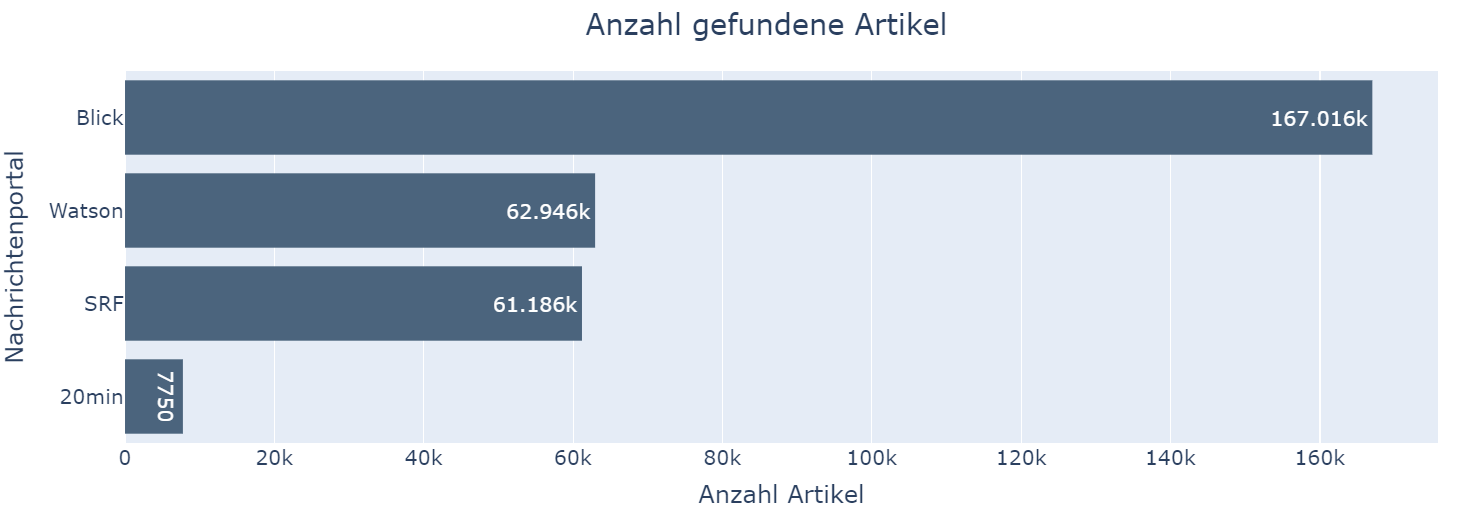
\includegraphics[width=1\linewidth]{./images/sum_all_2015-20230102.png}
		\caption{Anzahl Artikel pro Nachrichtenportal (unbereinigt), Stand 02.01.2023}
		\label{p2-count-articles}
	\end{center}
\end{figure}

Als Vorbereitung für die vorliegende Arbeit wurde eine grobe Methodik für das Extrahieren der Zitate, 
Personen und der geschlechtsbezogenen Informationen definiert. 
Die Methodik wurde inspiriert von der wissenschaftlichen Arbeit \citetitle{gender_gap_tracker} \cite{gender_gap_tracker}, 
welche auch die Grundinspiration dieser Bachelor Thesis ist.

\section{Literaturrecherche}
\subsection{Methodik der Literaturanalyse}

% Intro Text Begründung weshalb
Um die Resultate der Arbeit in Kontext setzen zu können und Inspiration von existierender Forschung zu erhalten,
war es für uns - aber auch für den Erfolg der Arbeit - wichtig, den aktuellen Stand der Forschung aufzuarbeiten.
Da die Menge an zur Verfügung stehenden Informationen sehr gross ist, war ein methodischer Ansatz gefragt.
Mithilfe unserer Betreuerin, Prof. Dr. Mascha Kurpicz-Briki,  haben wir die nachfolgende Herangehensweise besprochen, 
um die wichtigste Literatur abdecken zu können.

% Grundsätzliches Vorgehen
Die erarbeitete Methodik sah vor, dass als Erstes die relevantesten Portale von wissenschaftlichen Arbeiten
identifiziert werden sollten. Als wir diese definiert hatten, suchten wir als Nächstes einen Filter, der die Arbeiten auf etwa 100
potenziell relevante Artikel eingrenzen sollte. Aus diesem Kandidatenset wollten wir im Anschluss die Abstracts
durchlesen, um mindestens fünf und maximal 20 vergleichbare Arbeiten zu finden. Diese galt es dann, als Ganzes
zu lesen und in den nachfolgenden Unterkapiteln der Literaturrecherche zusammenzufassen.

\subsubsection{Auswahl der Portale}
Für die Auswahl der Portale stützten wir uns auf die Empfehlungen unserer Betreuerin und ergänzten diese mit
einer weiteren, uns bekannten Plattform. Schlussendlich durchsuchten wir die folgenden drei online Datenbanken mit
wissenschaftlichen Artikeln.
\begin{itemize}
    \item ACM\footnote{https://dl.acm.org}
    \item IEEE\footnote{https://ieeexplore.ieee.org}
    \item PLOS\footnote{https://journals.plos.org}
\end{itemize}
ACM und IEEE sind bekannte Datenbanken für wissenschaftliche Arbeiten aus der Informatik. PLOS ergänzt diese Auswahl mit einer sozialwissenschaftlichen Perspektive.

\subsubsection{Filterung der Portale}
Der Filter sollte so eng gefasst sein, dass er möglichst viele irrelevante Arbeiten ausschliesst, gleichzeitig
aber auch offen genug sein, damit wir eine genügend grosse Resultatliste erhalten. Um die geeignete Abfrage zu finden,
mussten wir Variationen des Filters ausprobieren, bis wir mit der Grösse des Resultats zufrieden waren.

Schlussendlich sollte unser Filter alle Artikel bezüglich \gl{gendergap} oder Bias in den Medien ausgeben.
Dies indem er die Abstracts nach Stichwörtern wie \enquote{gender}, \enquote{media} und \enquote{equality}
durchsucht. Damit wollten wir möglichst viele Arbeiten zum Thema \gl{gendergap} in den Online-Medien
finden. Die nachfolgende Abbildung \ref{plos-query} zeigt das entsprechende Query
für die Plattform PLOS.

\begin{figure}[h]
    \begin{verbatim}
                    (abstract:gender) AND 
                    (
                        (abstract:media) OR 
                        (abstract:news)
                    ) AND 
                    (
                        (abstract:gap) OR 
                        (abstract:inequality) OR 
                        (abstract:equality) OR 
                        (abstract:bias)
                    ) AND NOT
                    (
                        (abstract:"social media") OR 
                        (abstract:pandemic) OR 
                        (abstract:covid)
                    )
    \end{verbatim}
    \caption{Query zur Suche der relevanten Literatur}
    \label{plos-query}
\end{figure}

Da die ursprüngliche Liste viele Artikel zu Social Media Themen oder der Covid Pandemie enthielt, haben wir diese explizit
ausgeschlossen.

\subsubsection{Manuelle Aussortierung anhand der Abstracts}
Die Anwendung dieses Filters resultierte in einer Liste von 115 Arbeiten, deren Abstracts wir im Anschluss durchlasen
und dazu jeweils drei Fragen beantworteten.

\begin{enumerate}
    \item Befasst sich der Artikel mit Geschlechter(un)gleichheit in den Medien?
    \item Sind die untersuchten Medien textbasiert?
    \item Wurde die Auswertung mithilfe von \gl{nlp} durchgeführt?
\end{enumerate}

Schlussendlich entschieden wir uns dazu, diejenigen Arbeiten zu verwenden, bei denen wir die ersten zwei Fragen mit
\enquote{Ja} beantworten konnten. Die dritte Frage hätte uns geholfen, die Liste weiter einzuschränken, wären
mit den ersten zwei noch zu viele Arbeiten übrig geblieben.

Bei der Auswertung der Liste haben wir definiert, was wir unter textbasierten Medien alles einschliessen wollen.
Wir entschieden uns dazu, Nachrichtenportale und wissenschaftliche Arbeiten als Medien zu definieren, Schulbücher
und Kinderbücher jedoch aus dieser Definition auszuschliessen.

Nach dieser manuellen Suche nach den relevantesten Arbeiten enthielt unsere Liste noch acht Artikel aus den Portalen PLOS und ACM.

\subsubsection{Analyse der Arbeiten}
Diese acht Arbeiten haben wir im Anschluss gelesen und in den nachfolgenden Kapiteln zusammengefasst. Der Fokus lag
dabei auf den Themen der Geschlechter(un)gleichheit und den Analysemethoden, die der unseren ähneln. Für diese Arbeit irrelevante
Themen, die ebenfalls in den Artikeln beschrieben wurden, haben wir weggelassen, um die Arbeit nicht unnötig zu verlängern.

\subsubsection{Abweichungen von der Methode}
In zwei Fällen sind wir von der oben beschriebenen Methodik abgewichen. Wir kannten aus der Vorarbeit noch einen
weiteren Forschungsartikel, der uns relevant für unsere Arbeit schien. Dieser war in der Liste jedoch nicht enthalten, da er aus einem
anderen Portal stammt. Es handelt sich dabei um die Arbeit namens \citetitle{gender_bias_in_media} \cite{gender_bias_in_media}.
Die Zusammenfassung dieser Arbeit finden Sie zusätzlich zu den anderen in den nachfolgenden Seiten. Die zweite Abweichung
ist der Ausschluss der Arbeit \citetitle{iet-minoritized-communities} \cite{iet-minoritized-communities}. Es hat sich herausgestellt,
dass dieser Artikel keine Untersuchung beschreibt, sondern die Zusammensetzung und Stossrichtung einer geplanten Forschungsgruppe.
Diese wird unter anderem auch die Geschlechter(un)gleicheit in den Medien untersuchen. Im vorliegenden Paper ist jedoch noch kein
Ergebnis vorhanden. Diese Tatsache war im Abstract jedoch nicht klar beschrieben.
\subsection{The Gender Gap Tracker: Using Natural Language Processing to measure gender bias in media}

Die wissenschaftliche Arbeit \citetitle{gender_gap_tracker} \cite{gender_gap_tracker} von \citeauthor{gender_gap_tracker}
aus dem Jahr \citeyear{gender_gap_tracker} ist das Vorbild für die vorliegende Thesis. Im Rahmen
ihrer umfassenden Untersuchung der kanadischen, englischsprachigen Medien haben die Verfasser:innen nicht nur
den Gender Gap anhand der Anzahl Zitate pro Geschlecht und Nachrichtenportal untersucht, sondern 
auch neue Standards zur Messung und kontinuierlichen Überwachung der Repräsentation von Männern und Frauen in den
Medien geschaffen.

Aufgrund der ausführlichen Beschreibung ihrer Vorgehensweise und der geringen Eintrittshürde in
Bezug auf notwendiges vorprozessiertes Datenmaterial, kann diese Methodik auch gut in anderen Kultur-
und Sprachräumen nachgeahmt werden. Da dieses Projekt genau das vorhat, ist diese Arbeit in einem
grossen Detailgrad beschrieben.

\subsubsection{Ziele der Arbeit}

Das Ziel der Arbeit war es, den Unterschied in der Repräsentation der Geschlechter in den kanadischen
Medien sichtbar zu machen. Als Mass für die Repräsentation verwenden \citeauthor{gender_gap_tracker}
die Anzahl der Zitate in den Online-Nachrichtenportalen, die von Männern und Frauen publiziert werden.

Dazu haben sie eine Applikation entwickelt, die auf regelmässiger Basis die neusten Artikel
der Portale mittels Webcrawling herunterlädt und analysiert. Für die Untersuchung der Texte verwenden sie
verschiedene Arten von \gl{nlp}, über welche die folgenden Unterkapitel mehr Aufschluss geben sollen.

Schlussendlich visualisieren sie die Daten auf einer öffentlich zugänglichen Plattform in der Form einer
interaktiven Webapplikation
\footnote{https://gendergaptracker.informedopinions.org/}.
Die Resultate aus der Arbeit stammen direkt von dieser Software.

Die stets aktuellen Daten des \gl{ggt} werden bewusst öffentlich zur Verfügung gestellt, um den Medienschaffenden
Anreize zu verschaffen, für mehr Diversität in ihrer Berichterstattung zu sorgen. In der Arbeit
vergleichen sie den \gl{ggt} mit einem Fitness Tracker, der den Menschen helfen soll für ihrer
Fitness zu sorgen. Analog zu diesem Prinzip soll dieses Tool den Medienkonzernen mithilfe von Transparenz
und Rückverfolgbarkeit helfen, ihren \gl{genderbias} zu verringern.

\subsubsection{Zitate extrahieren}\label{ggt-method-citation}

Der Kern der Aufgabe des \gl{ggt} ist das Extrahieren von Zitaten. Die Entwickler:innen haben sich dazu eines vortrainierten, syntaktischen Parsers von Spacy bedient,
der Parsetrees aus Sätzen generieren kann. Die Software teilt die zu analysierenden Artikel also in die einzelnen Sätze auf und analysiert mit dem genannten Parser deren
einzelne Wörter. Mithilfe dieser Wörter und der dazugehörigen Bedeutung, die das Modell ihnen zuschreibt, kann die Applikation im Anschluss
zwei unterschiedliche Arten von Zitaten erkennen. Diese sind auch für die vorliegende Arbeit
von fundamentaler Bedeutung und wurden deshalb im Kapitel \ref{types-of-citations} im
Detail beschrieben.
\begin{enumerate}
    \item \gl{quote-syntactic}
    \item \gl{quote-floating}
\end{enumerate}

Diese Art Zitate zu unterscheiden erscheint auf den ersten Blick nicht intuitiv. So werden Zitate ja entweder in direkter, also mit Anführungs-
und Schlusszeichen, oder in indirekter Rede verfasst. Der naheliegende Ansatz wäre also die Unterscheidung nach diesen zwei Mustern. \citeauthor{SpronckNikitina+2019+119+159}
haben aber herausgefunden, dass ein syntaktischer Ansatz zum Parsen (mithilfe der Satzstruktur) bessere Resultate liefert, als semantisches Parsing (anhand von semantischen Merkmalen
wie Satzzeichen oder bestimmten Wörtern) \cite{SpronckNikitina+2019+119+159}. Aufgrund dieser Erkenntnis orientieren sie sich am syntaktischen Ansatz.

\subsubsection{Personen identifizieren und deren Geschlecht bestimmen}

Für ihre Auswertungen extrahieren die Forscher:innen alle Personen aus den Artikeln und bestimmen ihr Geschlecht.
Insbesondere interessieren sie sich für
\begin{enumerate}
    \item die Autorinnen und Autoren der Texte,
    \item die zitierten Personen (Quellen)
\end{enumerate}
aber auch generell für alle anderen Menschen, die im Text erwähnt werden.

Um Personen in den Artikeln zu finden, bedienen sie sich eines \textsl{\acrshort{ner}s (\textsl{Named Entity Recognizers})}. Dieser spezialisierte Parser kann aus Texten
Entitäten wie Personen, Orte und Firmen extrahieren. In diesem Fall werden nur die Personen weiterverarbeitet.

Das Resultat dieses Verfahrens ist eine Liste mit allen Wörtern und Satzteilen, die Personen repräsentieren. Diese Liste ist unbereinigt und
wird mithilfe eines \gl{cr} Algorithmus in zusammengehörige Gruppen aufgeteilt. So wird der \gl{ner} in einem Text über den
Bundesrat Berset viele unterschiedliche Repräsentationen dieses Mannes finden, wie zum Beispiel \enquote{Bundesrat Berset}, \enquote{er}, \enquote{Alain Berset}
etc. Da diese Nennungen alle der gleichen Person gelten, ist es für die Auswertung relevant, diese zu clustern.

Zur Identifikation des Geschlechts verwendet die Applikation eine Web API, die entweder nur mithilfe des Vornamens, oder mit Vornamen und Nachnamen, das Geschlecht
bestimmen kann. Einzelne Fälle, welche die API falsch zuordnet, führt die Applikation in einer dedizierten Liste.

\subsubsection{Evaluation}

Zur Qualitätssicherung haben die Forschenden kontinuierlich Messungen zur Performance ihrer Auswertungen durchgeführt. Das ermöglichte es ihnen, den Effekt von implementierten Verbesserungen
direkt messen zu können. Als Grundlage dazu dienten 14 repräsentative, manuell ausgewertete Artikel aus allen sieben verwendeten Nachrichtenportalen mit einer Mindestlänge von 3000 Zeichen.
Mithilfe dieses Datensatzes konnten sie die \gl{precision}, den \gl{recall} und den \gl{f1-score} für die Extraktion von Zitaten, Personen und Verben bestimmen.

\subsubsection{Resultate}
% Absoluter Gender Gap
Die Resultate der Arbeit können einen klaren \gl{gender-bias-distribution} in den untersuchten
Onlineartikel aus sieben kanadischen Medienhäusern feststellen. So sind die Zitate in ihrem Datensatz
in einem Durchschnitt über zwei Jahre (01.10.2018 - 30.09.2020) in nur 29\% der Fälle Frauen zuzuordnen.
Die verbleibenden 71\% sind Zitate von Männern.

Der Unterschied in der Verteilung der Zitate zwischen den Geschlechtern variiert zwischen den Medienhäusern,
wobei CBC News mit 33\% der Zitate am besten und The Globe and Mail mit 23\% am schlechtesten abschneiden.

Aus ihren Daten ist ersichtlich, dass Frauen während der Coronapandemie häufiger zitiert wurden als zuvor.
Die Autorinnen und Autoren weisen auf die Tatsache hin, dass Frauen in den Gesundheitsämtern häufiger vertreten sind als in
anderen Bereichen der Arbeitswelt und dass eine ausgeglichene Repräsentation der Geschlechter in wichtigen
Ämtern den \gl{gendergap} zu verringern scheint.

% Gender Gap unter wichtigen Personen
Die für diese Auswertung gesammelten Daten boten auch die Möglichkeit, Untersuchungen zu den am häufigsten zitierten
Menschen zu machen. So haben die Forscher:innen einen Ausschnitt der Top 15 zitierten Personen aus dem Datenset genauer
untersucht. Diese haben sie im Anschluss Kategorien wie Politik, öffentlicher Gesundheit und Privatwirtschaft zugewiesen.
Die meistzitierte Frau in dieser Liste würde mit 2'239 Zitierungen gerade mal den 8 Platz in der Rangliste der Männer
einnehmen. Interessanterweise sind alle 15 Vertreter der meistzitierten Männer im Sektor der Politik tätig. Auch bei den
Frauen sind die meisten Politikerinnen. Drei sind aus dem Bereich der öffentlichen Gesundheit und eine aus der Privatwirtschaft.
Dass es drei Vertreterinnen aus dem Gesundheitssektor in die Top 15 meist zitierten Frauen im Datensatz schaffen, weist ebenfalls
darauf hin, dass eine ausgeglichenere Frauenquote in für die Öffentlichkeit interessanten Bereichen den Geschlechtergraben verkleinern
könnte.


% Gender Gap nach Bereich der Gesellschaft
Eine weitere Analyse der Wissenschaftler:innen zeigt die Aufteilung der Zitate nach Geschlecht und Tätigkeitsgebiet der Quelle.
Die tabellarische Auswertung zeigt, dass die meistzitierten Männer Politiker (73.8\%), Sportler (7.7\%) und Regierungsangestellte sind.
Bei den Frauen finden sich die meisten Zitate in den Tätigkeitsgebieten Politik (52.6\%), Gesundheit (16.7\%) und Exekutive (8.3\%) (Regierungsangestellte).
Auch hier fällt wieder auf, wie massiv weniger Frauen zitiert werden. So werden Politiker 103'378 und Politikerinnen 29'007 Mal zitiert,
Sportler 10'723 und Sportlerinnen 1'415 Mal und Regierungsangestellte Männer 9'175 und Frauen 4'583 Mal. Nur in den Bereichen öffentliche Gesundheit,
NGO's und Wissenschaft werden Frauen leicht häufiger zitiert.

Eine interessante Nebenerkenntnis dieser Auswertung ist die Tatsache, dass insgesamt weniger Zitate von Frauen in Online-Nachrichtenportalen
erscheinen als von Männern, jedoch absolut gesehen mehr individuelle Frauen zitiert werden. Das bedeutet, dass die Anzahl Zitate pro Mann
deutlich höher ist als die Anzahl Zitate pro Frau.

Sie erkennen das Muster, dass Männern mehr Raum gegeben wird als Frauen und einige wenige Kategorien den grössten Teil der Berichterstattung
dominieren. Die Forscher:innen spekulieren aufgrund dieser Erkenntnis, dass die Daten einer Pareto Verteilung unterliegen. Also dass das
grösste Hindernis mehr von Frauen zu hören die Bevorzugung derer ist, die bereits sehr viel Raum einnehmen.

% Gender Gap nach Geschlecht des Authors
In einer weiteren Auswertung haben \citeauthor{gender_gap_tracker} den Zusammenhang zwischen dem Geschlecht des
Autors oder der Autorin und der Anzahl und Verteilung der Zitate von Männern und Frauen untersucht. Sie wollten
damit herausfinden, ob Frauen häufiger weibliche Quellen zitieren als Männer. In der Tat scheinen Journalistinnen
häufiger Frauen zu zitieren als Journalisten. Während Männer im Schnitt nur in einem Viertel (25\%) ihrer Zitate auf Frauen
zurückgreifen, sind es bei den Frauen immerhin 34\%. Daraus schliessen die Autorinnen und Autoren, dass ein Teil der Lösung zum
Gender Gap in der Erhöhung der Quote von Reporterinnen besteht. Nicht nur, weil sie in selbst geschriebenen Artikeln
häufiger Frauen zitieren, sondern weil sie auch in gemischten Teams einen positiven Einfluss auf die Wahl der Quellen
ausüben, wie die Auswertung zeigt.

% Applikation
Die Applikation, die auf täglicher Basis die für diese Auswertungen notwendigen Daten aggregiert, ist nach wie vor im Einsatz und wird - wenn auch sporadisch, 
doch immer wieder weiterentwickelt. Die aktuellsten Auswertungen sind in interaktiver Form auf \href{https://gendergaptracker.informedopinions.org/
}{GenderGapTracker.InformedOpinions.org} zu finden. Der Code dazu ist öffentlich auf \href{https://github.com/sfu-discourse-lab/GenderGapTracker}{GitHub} einsehbar.


\subsubsection{Weiterentwicklung des Gender Gap Trackers}
Nach der Fertigstellung des Papers im Jahr \citeyear{gender_gap_tracker}, wurde die Applikation um die Möglichkeit, auch französische Artikel
zu analysieren, erweitert. Damit analysiert der \gl{ggt} zum aktuellen Stand sieben englisch- und sechs französischsprachige Nachrichtenportale.

Da die Release Notes auf GitHub erst seit September 2022 geführt werden, bleiben wohl viele neue Features, die in der Arbeit nicht beschrieben sind,
verborgen. Die Entwickler:innen sind jedoch fleissig am \gl{refactorn} und scheinen den \gl{ggt} regelmässig zu warten und weiterzuentwickeln.
\subsection{Does Gender Matter in the News? Detecting and Examining Gender Bias in News Articles}

In ihrer Arbeit \citetitle{does-gender-matter-in-the-news} \cite{does-gender-matter-in-the-news} erforschten \citeauthor{does-gender-matter-in-the-news}
den impliziten und expliziten Bias in Abstracts von Nachrichtenartikeln aus zwei Datensets (\gl{mind}\footnote{https://msnews.github.io/}, \gl{ncd}
\footnote{https://www.kaggle.com/rmisra/news-category-dataset}) auf Bias zwischen den
Geschlechtern. Im Speziellen untersuchten sie dabei den \gl{gender-bias-distribution}, den \gl{gender-bias-content} und den \gl{gender-bias-wording}.

Das \gl{mind} Dataset besteht aus ungefähr 160'000 englischsprachigen Nachrichtenartikeln mit Text, Titel, Abstract und Kategorien. Das Datenset enthält
auch anonymisierte User Logs, die für diese Auswertung jedoch irrelevant sind. \gl{ncd} ist ein Kaggle Dataset bestehend aus etwa 210'000 englischsprachigen
Schlagzeilen mit dazugehörigen Abstracts.

% Methodik mit Attribute words erklären

Im ersten Experiment untersuchten die Forschenden den \gl{gender-bias-distribution}. Dazu teilten sie die Abstracts beider Datensets
in drei Kategorien auf: Männlich (M), Weiblich (F) und Neutral (N) und verglichen die Anzahl Abstracts in den jeweiligen Kategorien
anschliessend tabellarisch. Um die Aufteilung vorzunehmen, bedienten sie sich eines Datensets von 465 geschlechterbezogenen \gl{possessive-noun}s und
357 geschlechterspezifischen \gl{attribute-word}s. Mit diesem Experiment konnten sie im \gl{mind} Datenset einen klaren \gl{gender-bias-distribution}
von 53.9\% zugunsten der Männer nachweisen. Das andere Datenset schnitt mit einem \gl{gender-bias-distribution} von 14.5\% zugunsten der Männer nur
deshalb besser ab in der absoluten Verteilung, weil Frauen in den Kategorien \enquote{Style \& Beauty},
\enquote{Parenting} und \enquote{Entertainment} stark übervertreten sind, was auf einen Bias in der Art der Präsentation von Frauen hindeutet,
wie auch das zweite Experiment zeigt.

Dieses soll den \gl{gender-bias-content} messen, in dem es die Häufigkeit vergleicht, mit der Frauen und Männer in den Kontexten Familie und Karriere
vorkommen. Dazu setzen sie zwei weitere \gl{attribute-word}s Sets ein, mit denen sie die geschlechterbezogenen Abstracts den gefragten
Kontexten zuweisen können. Das Resultat zeigt, dass Frauen im \gl{mind} Dataset 16.21\% weniger häufig mit Karriere assoziiert werden, als Männer. Im NCD Datensatz
ist der Unterschied mit 8.51\% halb so gross. Im Gegenzug werden sie häufiger im Kontext von Familie beschrieben. Im \gl{mind} Datensatz 4.1\% häufiger und im
NCD Datensatz 3.19\% häufiger. Diese Erkenntnis wird auch durch das dritte Experiment gestützt.

In diesem Experiment untersuchen die Forschenden basierend auf Sentiment Analysis und \gl{cra} den \gl{gender-bias-wording}.
Mithilfe des Tools \gl{vader} extrahierten sie aus den nach Geschlecht aufgeschlüsselten Abstracts diejenigen mit positiver Benotung des Algorithmus.
Anschliessend liessen sie den \gl{cra} die 20 wichtigsten Wörter in den jeweiligen Sammlungen als Graph darstellen. In diesem ist die Wichtigkeit des
jeweiligen Wortes als Grösse der Knoten ersichtlich. Wörter, die in denselben Kontexten vorkommen sind durch Kanten verbunden.
Das Resultat deutet auf einen starken \gl{gender-bias-wording} hin. Während die wichtigsten 20 Wörter bezogen auf Männer \enquote{president},
\enquote{manager} und \enquote{mayor} beinhalten, beginnt die Top 20 Liste bei den Frauen mit \enquote{wife}, \enquote{mother} und \enquote{beloved}.
Dieses Experiment stützt also auch die Erkenntnis aus dem zweiten Experiment, dass Frauen in den Medien besonders im Kontext der Familie,
ihres Ehemannes oder ihres Körpers porträtiert werden und nicht wie die Männer im Zusammenhang mit Politik, Wirtschaft oder Karriere.

Um die oben beschriebenen Experimente durchzuführen haben \citeauthor{does-gender-matter-in-the-news} einiges an Datenaufbereitung betrieben.
Damit künftige Forschende einen einfacheren Zugang zu solchen Daten haben, veröffentlichten sie diese im Rahmen der Arbeit für die freie Verwendung
in der Forschung \footnote{https://github.com/daconjam/Detecting\_Gender\_Bias}.



\subsection{DIANES: A DEI Audit Toolkit for News Sources}
Die Autoren und Autorinnen der Arbeit \citetitle{10.1145/3477495.3531660} \cite{10.1145/3477495.3531660} haben ein Audit Toolkit entwickelt,
um Journalist:innen und Reporter:innen von Nachrichtenportalen dabei zu helfen, 
den Anteil der Quellenvielfalt (z.B. Geschlecht und Rasse) für Zitate in ihren Artikeln zu verbessern.
Laut den Verfasser:innen der Arbeit wird in professionellen Nachrichtenmedien immer betont, wie wichtig die Vielfalt der Perspektiven ist, 
aber in der Praxis wird dem nur wenig Beachtung geschenkt.
Daher sind die Nachrichtenmedien unter ethische Kritik geraten im Rahmen der neuen Normen für Vielfalt, Gleichberechtigung und Integration, 
im englischen \gl{dei}.
Das Toolkit soll die Medienschaffenden dabei unterstützen, diesen Normen mehr Beachtung zu schenken.
\gl{dianes} ist ein \gl{dei} Toolkit, das eine NLP-Pipeline im Backend zur Extraktion von Zitaten, Sprechern, Titeln und Organisationen
aus Nachrichtenartikeln verwendet und diese in Echtzeit verarbeitet. 

Im Frontend unterstützt \gl{dianes} eine Vielzahl von Benutzeranfragen zum \gl{dei} Audit auf der Grundlage der im Backend extrahierten Informationen. 
Auf dem Artikel Dashboard können Medienschaffende ihren Artikeltext als Entwurf eingeben und 
dann die entsprechenden Informationen zur Quellenvielfalt in diesem Artikel abrufen.
Das Dashboard der Quellenvielfalt ist dazu da, die \gl{dei} Daten für einen ausgewählten Zeitraum von allen Artikeln zu visualisieren.

Das \gls{api} implementiert die Möglichkeit, alle Zitate, Namen, Geschlechter sowie Titel der Sprecher:innen zu extrahieren, 
die in Artikeltexten vorkommen, welche der \gls{api} gesendet werden.

% Backend Text
Das Backend Modul nimmt den Nachrichtenartikel als Input und extrahiert die Zitate und Sprecher:innen mit ihren Titeln und
prognostiziert dann Geschlecht und Rasse/Ethnie dieser zitierten Person.
Das Modul ist in folgende vier Stages unterteilt, von welchen die ersten zwei Stages  
die Standford CoreNLP Bibliothek \footnote{https://stanfordnlp.github.io/CoreNLP/} nutzen.

\subsubsection{Text Processing}
In der \enquote{Text Processing} Phase werden zunächst unnötige Informationen aus dem Text gefiltert wie \ashort{xml} Tags.
Nach dem Filtern wird der Text tokenisiert und im nächsten Schritt wird \gl{pos} Tagging angewendet um z.B. zu bestimmen,
ob die einzelnen Wörter (Tokens) Verben oder Substantive sind. 
Danach wird eine \gl{lemming} durchgeführt, um jedes Wort auf seine Grundform zu reduzieren.

\subsubsection{NLP Analysis}
Der \enquote{NLP Analysis} Schritt enthält die folgenden spezifischen Komponenten.
Die Satzspaltung teilt den Text in Sätze auf. Dies wird anhand des CoreNLP Regelwerks gemacht.
Mit \gl{ner} werden Personen, Titel und Organisationen im Text bestimmt.
Dependency Parsing analysiert die grammatikalischen Beziehungen zwischen Wörtern in einem Satz 
und extrahiert textuelle Beziehungen auf Basis der Abhängigkeiten.
Die \gl{cr} findet Erwähnungen der gleichen Entität in einem Text, z.B. wenn 
sich \enquote{Anne} und \enquote{sie} auf dieselbe Person beziehen.
\gl{kbp} wird verwendet um Titel und Organisationen einer Person zu finden, wenn diese
im Text vorkommen. 

\subsubsection{Annotations}
In diesem Teil werden Annotationen erstellt für Zitate, Sprecher:innen und ihre Titel und 
Organisationen auf der Grundlage der vorherigen \gl{nlp} Analyse. 
Wenn bei einem Zitat ein Anführungszeichen oder Schlusszeichen fehlt, hat CoreNLP den Text bis 
zum nächsten Anführungszeichen/Schlusszeichen des nächsten Zitates als Zitat Inhalt deklariert, was die Genauigkeit der Zitat-Auflösung verringern kann.
Um dieses Problem zu umgehen, arbeiteten die Entwickler:innen mit der Anzahl Wörter in vorgängigen Zitaten.
Zitate mit über 100 Wörter oder unter fünf Wörter wurden für die Auswertung ausgeschlossen.
Die Entwickler:innen machten die Erfahrung, dass CoreNLP Probleme hatte und oft die falsche Person zum Zitat zuwies.

\subsubsection{Representation Recognition:}
Diese Phase dient dazu Geschlecht und Rasse/Ethnie der zitierten Person zu definieren.
Diese zwei Repräsentationsattribute von \gl{dei} sind die entscheidenden Informationen zum Verständnis der Repräsentativität der Nachrichtenbeschaffung von \gl{dianes}.
Das Geschlecht wurde mit der Gender API \footnote{https://gender-api.com/} bestimmt.
Es gibt viel weniger existierende Arbeiten zur Vorhersage der Rasse/Ethnizität
einer Person mit einem Namen, und die Aufgabe ist anspruchsvoller als Geschlechtserkennung.
Darum wurde zur Vorhersage der Rasse/Ethnizität einer Person ein eigenes \gl{ml} Model implementiert und trainiert, 
welches als Input den Namen der Person braucht.
Der Datensatz, der zum Trainieren des Rassendetektors verwendet wurde, stammt von dem United States Census Bureau aus den Jahren 2000 und 2010. 
Er enthält insgesamt 151'670 eindeutige Namen in sechs Kategorien (White, African, American, American Indian, Alaska Native, Asian, Native
Hawaiian und Other Pacific Islander).

\gl{dianes} wurde zum Zeitpunkt der Veröffentlichung der Arbeit von mehreren Redaktionen in der Praxis getestet.
\subsection{The gender gap in commenting: Women are less likely than men to comment on (men's) published research}
Die Studie \citetitle{gender_gap_in_commenting} \cite{gender_gap_in_commenting} behandelt den \gls{gendergap}
im Kommentieren von veröffentlichten Forschungsartikeln. 
Die Autorinnen und Autoren gehen der Frage nach, ob auch das Kommentieren von veröffentlichten Forschungsartikeln geschlechtsspezifisch ist.
In der Studie haben die Verfasser:innen anhand von 1'350 Kommentaren zu 1'236 Forschungsartikeln, 
welche in den Fachzeitschriften - \gl{pnas} und Science - veröffentlicht wurden festgestellt,
dass es eine geschlechtsspezifische Diskrepanz bei den Verfasser:innen von Kommentaren gibt.

Die Autorinnen und Autoren haben sich gefragt, wieso Frauen seltener Kommentieren als Männer.
Sie haben die Theorie aufgestellt, dass es beim Kommentieren um Herausforderung, Risiko und Belohnung geht.

\subsubsection{Allgemeine Risikoaversion}
Wenn eine Person sich entscheidet, einen für alle sichtbaren Kommentar unter einen veröffentlichten Forschungsartikel zu schreiben,
geht sie auch das Risiko ein, den eigenen Ruf zu schädigen.
Das Kommentieren setzt die Bereitschaft voraus, die Überlegenheit der eigenen wissenschaftlichen Erkenntnisse über die eines anderen zu behaupten.
Die Forscher:innen treffen die Annahme, dass Wissenschaftler:innen mit der Abgabe von Kommentaren warten, 
bis sich ihre Karriere besser etabliert hat.
Da Frauen meist auf tieferen Karriere Stufen sind als Männer, verfassen sie deshalb weniger Kommentare, so ihre Theorie.
In diesem Fall wäre der Unterschied bei der Verteilung der Geschlechter im Kommentieren von Forschungsartikeln ein Pipeline-Effekt.

\subsubsection{Geschlechtsspezifische Risikoaversion}
Möglicherweise könnte das Geschlecht die relative Abwägung der Risiken und der Chancen durch einen Kommentar beeinflussen.
Aus jahrzehntelanger Forschung ist bekannt, dass Männer risikofreudiger sind als Frauen 
\cite{gender_differences_in_risk_taking,gender_and_culture,self_promotion_risk_factor_for_women,gender_differences_automatic_in-group_bias,gender_differences_in_risk_assessment}. % 38
Daraus ist zu schliessen, dass sich Frauen mehr Sorgen über die negativen Folgen machen, wenn sie einen Forschungsartikel kommentieren wollen
und dies darum seltener tun.
Die Autorinnen und Autoren erwarten auch, dass die geschlechtsspezifischen Unterschiede bei der Kommentierung schwächer ausfallen, 
wenn der Zielartikel von einer jüngeren Person verfasst wurde und somit das Risiko, sich gegen sie zu stellen, geringer ist.

\subsubsection{Geschlechtsspezifisches Risiko}
Denkbar ist auch, dass die Folgen von Kommentaren geschlechtsspezifisch sind.
Frauen und Männer werden für dasselbe Verhalten unterschiedlich bestraft und belohnt.
Von Frauen wird erwartet, dass sie gemeinschaftlich und nicht durchsetzungsfähig sind
\cite{burgess1999women,eagly2002role}. % 40
Bei Männer hingegen hat die Gesellschaft die Erwartung, dass sie durchsetzungsfähig und wettbewerbsorientiert sind.
Ein Verstoss gegen diese geschlechtsspezifischen Stereotypen führt in der Regel zu Missbilligung
\cite{self_promotion_risk_factor_for_women,mclaughlin2012sexual,mark_of_a_womans_record,rudman2008backlash}. % 43
Wenn Frauen als durchsetzungsfähig wahrgenommen werden und in männerdominierten Bereichen Erfolg haben, 
sinkt ihre \enquote{Beliebtheit} in der Regel mit negativen sozialen und wirtschaftlichen Folgen
\cite{self_promotion_risk_factor_for_women,mclaughlin2012sexual,mark_of_a_womans_record,rudman2008backlash}. % 43
Während Kommentare im Allgemeinen für Frauen unverhältnismässig riskant sein könnten, 
dürfte dies noch ausgeprägter sein, wenn es sich bei der Zielperson um einen männlichen Wissenschaftler handelt, 
da dies die vermeintliche Überlegenheit von Männern infrage stellt. 
Dies bedeutet, dass Frauen im Vergleich zu männlichen Kommentatoren wahrscheinlich weniger Artikel angreifen, 
die von Männern verfasst wurden.

\subsubsection{Geschlechtsspezifische Fürsorge unterdrückt Herausforderungen}
Frauen gelten oft als das fürsorglichere Geschlecht \cite{marsh2019caring}. % 46
Das Kommentieren ist nicht unbedingt eine angenehme Praxis, da es die Arbeit eines anderen infrage stellt. 
Es ist durchaus denkbar, dass potenzielle Verfasser:innen von Kommentaren befürchten, 
dass ihr Kommentar negative Folgen für die Betroffenen haben könnte.
Dies könnte die Quote der Kommentare von Frauen senken.

%Die Resultate der Untersuchung der Kommentare zeigt, dass nur 15 \% der Kommentare eine weibliche Erstautorin haben 
%gegenüber 26 \% der Artikel welcher von Frauen verfasst wurden, ein signifikanter Unterschied (p < .001).
Die Resultate der Untersuchung zeigen, dass unter den jüngeren, gefährdeteren Wissenschaftler:innen der Anteil der Autorinnen 
sowohl bei Kommentaren als auch bei Artikeln höher ist, wahrscheinlich weil Frauen in den unteren akademischen Rängen stärker vertreten sind.
%Zwar ist der geschlechtsspezifische Unterschied bei der Verfasserschaft von Kommentaren und Artikeln bei denjenigen, 
%die keine korrespondierenden Autoren sind, tatsächlich größer, wie es das Argument der geschlechtsspezifischen Risikoaversion vorhersagt, 
%doch ist dieser Unterschied auf konventionellem Niveau nicht signifikant (p = .09).

% noch mal schauen ob das nicht zu viel infos sind
Wenn eine grössere Risikoaversion der Grund für die geringere Rate an Kommentaren von Frauen ist, 
erwarten die Forscher:innen auch eine geringere geschlechtsspezifische Diskrepanz bei der Verfasser:innenschaft von Kommentaren, 
wenn der Erstautor relativ machtlos ist, da dies die Risiken beim Kommentieren im Allgemeinen weniger auffällig machen sollte. 
Umgekehrt, wenn Frauen insgesamt weniger kommentieren, weil sie sich mehr Sorgen machen, 
die Karriere anderer zu schädigen (geschlechtsspezifische Fürsorge drückt die Herausforderung), 
wird der geschlechtsspezifische Unterschied bei der Kommentierung zugunsten der Männer grösser sein, wenn die Zielperson stärker gefährdet ist. 
Tatsächlich sind die geschlechtsspezifischen Unterschiede in der Wahrscheinlichkeit, auf solche Artikel zu zielen, 
gering und statistisch nicht signifikant. Die Ergebnisse deuten also darauf hin, 
dass die unterschiedliche Risikoorientierung von Frauen an sich (sei es für sie selbst oder für die Zielpersonen) wahrscheinlich 
nicht der Grund für ihre geringere Rate an Kommentaren ist. 

Während sowohl Männer als auch Frauen eher auf Artikel abzielen, die zuerst von Männern verfasst wurden, 
ist dies bei Männern deutlich ausgeprägter. Da Frauen unter den Autoren von \gl{pnas}- und Science-Artikeln unterrepräsentiert sind, 
würde dies an sich schon die Gesamtzahl der Kommentare von Frauen im Vergleich zu Männern senken.
Es lässt sich nicht feststellen, ob diese Dynamik darauf zurückzuführen ist, 
dass Frauen andere Frauen als Zielpersonen bevorzugen (wie das Argument des geschlechtsspezifischen Risikos behauptet) 
oder dass Männer andere Männer überproportional bevorzugen (oder eine Kombination aus beidem). 
Es ist auch möglich, dass Frauen weniger als Männer auf Artikel abzielen, die von Männern geschrieben wurden, 
und zwar nicht aufgrund unterschiedlicher Konsequenzen, 
sondern weil ihr Fachwissen in Bezug auf die Arbeit von Frauen relevanter ist.
Dies weil Arbeiten, welche von Frauen verfasst wurden, auch ein wenig die Sichtweisen einer Frau repräsentieren.

Letztendlich konnte mit den Daten nicht direkt überprüft werden, ob Frauen mehr negative Konsequenzen erleiden, 
wenn sie den aktuellen Stand infrage stellen. Angesichts der aufgedeckten Muster und der mangelnden Unterstützung 
für die anderen Argumente bleibt dies jedoch eine plausible Erklärung für die niedrigere Rate an Kommentaren von Frauen.

% Conclusion
Die Studie kommt zu dem Ergebnis, dass sich Frauen seltener an akademischen Kommentaren beteiligen.
Eine Diskrepanz, welche die geschlechtsspezifischen Unterschiede bei der Veröffentlichung von Artikeln übersteigt. 
Diese Diskrepanz kann nicht durch Schwankungen im fachspezifischen Geschlechterverhältnis erklärt werden. 
Auch die Überrepräsentation von Frauen in den für Karriererisiken empfindlichsten Positionen oder 
eine grössere allgemeine Sensibilität für Risiken für andere können die Diskrepanz nicht erklären. 
Frauen richten auch einen geringeren Anteil ihrer Kommentare auf die Forschung von Männern als Männer. 
Zusammengenommen stimmen die beiden Ergebnisse am ehesten mit dem Argument überein, 
dass die geringere Anzahl von Kommentaren von Frauen auf die geschlechtsspezifischen Kosten zurückzuführen ist, 
die mit der Infragestellung massgeblicher Forschung verbunden sind, 
insbesondere wenn es um die Infragestellung traditioneller Statushierarchien geht. 
Dieses Argument kann aber mit den Daten nur indirekt überprüft werden.
 
Diese geschlechtsspezifischen Muster bei akademischen Kommentaren könnten den wissenschaftlichen Austausch 
zwischen Männern und Frauen behindern und Frauen innerhalb der wissenschaftlichen Gemeinschaft weiter marginalisieren. 
Wenn Expertinnen ausgeschlossen werden, fehlt es der akademischen Gemeinschaft als Ganzes an frischen Ideen und vielfältigen Meinungen.
\subsection{Using citation network analysis to enhance scholarship in psychological science: A case study of the human aggression literature}

In dem Forschungsartikel \citetitle{citation-network} untersuchten \citeauthor{citation-network} mithilfe einer graphbasierten Analyse
die Zusammensetzung der Forschungsgemeinschaft zum Thema \enquote{Aggression} \cite{citation-network}. Neben der Untersuchung zu den
einflussreichsten Gemeinschaften auf diesem Feld wollten die Forscher:innen ausserdem herausfinden, ob ihre Netzwerkanalyse dazu beitragen kann,
den \gl{genderbias} beim Zitieren von wissenschaftlichen Arbeiten zu reduzieren.

Der Grund für diesen Bias, so mutmassen die Autorinnen und Autoren des Artikels, liegt in der Art wie die Relevanz von wissenschaftlichen Arbeiten beurteilt wird.
So werden aktuell diejenigen Papers als am relevantesten eingestuft, die am meisten zitiert wurden. Dieser Fokus auf der Anzahl Zitierungen begünstigt
vermutlich einen Bias zum Vorteil von etablierten Forschungsgemeinschaften und führt zu einer Unterrepräsentation von anderen wichtigen Forschungsgruppen,
so \citeauthor{citation-network}. Dass dieser Ansatz im Falle von Publikationen im Bereich der Astronomie \gl{genderbias} begünstigt, haben
\citeauthor{citation-astronomy} bewiesen \cite{citation-astronomy}.

In ihrem Experiment vergleichen \citeauthor{citation-network} den Frauenanteil unter den Autorinnen und Autoren aus den Top 75 Artikeln, ausgewählt nach drei Methodiken.
\begin{enumerate}
    \item Anzahl Zitierungen
    \item Kompositrangierung
    \item Kompositrangierung mit Einbezug der Gemeinschaften
\end{enumerate}

Die erste Methodik, \enquote{Anzahl Zitierungen}, entspricht dem Status Quo. Also, dass die wichtigsten Arbeiten anhand der absoluten Anzahl der Zitierungen
identifiziert werden. Die zweite Methodik nennen die Forschenden \enquote{composite score}. Auf Deutsch wäre das eine \enquote{Kompositrangierung}.
Diese besteht aus sechs Teilbewertungen (Komposite) zur Messung der Zentralität einer Arbeit im gesamten Zitatnetzwerk.
Der letzte Ansatz ist eine Erweiterung der Kompositrangierung und teilt allen Gemeinschaften im Graphen gleich viele Ranglistenplätze zu. Diese werden dann anhand der
\enquote{Kompositrangierung} sortiert.

Die Auswertung betrachtet die 75 bestplatzierten Arbeiten und vergleicht den Anteil der Autorinnen untereinander. Während dieser gemessen an der traditionellen Methode
gerade mal 16\% (12) beträgt, sind es bei der \enquote{Kompositrangierung} bereits 20\% (15) und unter Berücksichtigung der Gemeinschaften gleich 32\% (24).
Die \enquote{Kompositrangierung mit Einbezug der Gemeinschaften} hat im verwendeten Datensatz also zu einer Verdoppelung der Quote von Autorinnen geführt. 
\citeauthor{citation-network} bemerken, dass diese Art der Relevanzbewertung nicht nur dabei helfen kann, unterrepräsentierte Gemeinschaften in der Forschung besser 
sichtbar zu machen, sondern auch den \gl{gendergap} zu reduzieren.

Leider bietet die Arbeit keine Auskunft zum Anteil der Autorinnen über das gesamte Datenset, was das Einordnen ihrer Zahlen erschwert. So ist es nicht möglich zu beurteilen,
ob der Anteil der Arbeiten, die von Frauen verfasst wurden, insgesamt mehr oder weniger als 32\% ausmacht und wie gross oder klein der \gl{gendergap} damit noch immer ist.
\subsection{A Large-Scale Test of Gender Bias in the Media}
Die Autorinnen und Autoren der Arbeit \citetitle{gender_bias_in_media} \cite{gender_bias_in_media} untersuchten den Gender Bias in einem
Datensatz von \enquote{Lydia news analysis system} \cite{lydia}. Dieser enthält zeitgestempelte Nennungen von Personen aus
mehr als 2000 gescannten oder digitalen Zeitungen, Magazinen und online Nachrichtenartikeln aus den Jahren 2004 bis 2009.
Die Quellen stammen vorwiegend aus dem US amerikanischen Raum. 
Sie stellen fest, dass Frauen im Vergleich zu Männern in ähnlichen Positionen und aus denselben Berufsschichten ein grösseres öffentliches 
Interesse geniessen, aber weniger Medienberichterstattung erhalten.

In über 10'000 untersuchten Paaren von Männern und Frauen gleichen Alters, die im selben Sektor tätig sind und gleiches öffentliches
Interesse geniessen, haben die Forschenden einen Unterschied von 46\% in der Anzahl jährlicher Nennungen zugunsten der Männer gemessen.
So wurden die Frauen aus den gebildeten Paaren 300 Mal erwähnt und die Männer 826 Mal.

% Jüngste Studien, in denen grosse Zeitungsdatensätze analysiert wurden, deuten darauf hin, 
%dass der Anstieg des Anteils der Zeitungsberichterstattung über Frauen in letzter Zeit fast zum Stillstand 
%gekommen ist (Gallagher 2010; Macharia 2015). Das Verhältnis von Frauen zu Männern in Zeitungsartikeln hat sich 
%bei etwa 1:4 stabilisiert (Macharia 2015; Shor et al. 2014b, 2015), während das Verhältnis bei Gesichtsbildern 
%zwischen 1:1,5 und 1:4 liegt (Jia et al. 2016). 

Die Forscher:innen argumentieren mit den zwei folgenden Erklärungen wieso die Berichterstattung über Männer unverhältnismässig ist.
Die erste Erklärung könnte die berufliche Ungleichheit zwischen Frauen und Männer sein.
Studien haben gezeigt, dass Männer häufiger vertreten sind in Machtpositionen
\cite{gender_inequality_in_labor_markets,gender_revolution}. 
Besonders in Bereichen, denen die Medien grössere Aufmerksamkeit schenken.
Daraus folgt natürlich, dass die Mainstream-Medien mehr über Männer als über Frauen berichten.

Als zweite Erklärung erkennen die Forscher:innen, dass die Ungleichheit in der Berichterstattung ein unverhältnismässig grosses öffentliches Interesse an Männern widerspiegeln könnte.
Dies kann darauf zurückzuführen sein, dass das Publikum Nachrichten über Männer bevorzugt oder dass Männer ein grösseres Interesse wecken, 
weil sie Verhaltensweisen an den Tag legen, die die Öffentlichkeit für berichtenswert hält.

% Die Forscher:innen versuchen, die folgenden drei Forschungsfragen zu beantworten:
% \begin{enumerate}
%     \item Erhalten Frauen weniger Berichterstattung als Männer, selbst wenn sie gleichwertige Positionen oder Leistungen in Politik, Wirtschaft, Unterhaltung, Sport und anderen sozialen und beruflichen Bereichen erreicht haben? 
%     \item Unterscheidet sich das öffentliche Interesse an Männern und Frauen, die eine ähnliche Position erreicht haben? 
%     \item Erhalten Frauen selbst dann weniger Medienaufmerksamkeit als vergleichbare Männer, wenn man sowohl ihre strukturelle Positionierung als auch das öffentliche Interesse berücksichtigt, das sie auf sich ziehen?
% \end{enumerate}

% Why Might Successful Women Receive Less Coverage Compared With Successful Men? Causal Mechanisms and Research Hypotheses

Die Forscher:innen gehen davon aus, dass Ungleichheiten in der Medienberichterstattung über Männer und Frauen in erster Linie 
auf eine der folgenden drei Hauptkategorien von Erklärungen zurückzuführen sind:
\begin{itemize}
    \item strukturelle Ungleichheiten in der Arbeitswelt und in hochrangigen Positionen 
    \item Ungleichheiten in Bezug auf öffentliches Interesse und Nachrichtenwert bei gleichwertigen Positionen
    \item Medienspezifische Faktoren: Voreingenommenheit und Diskriminierung in der Medienberichterstattung
\end{itemize}

\subsubsection{Strukturelle Ungleichheiten in der Arbeitswelt und in hochrangigen Positionen}
Frauen haben oft einen eingeschränkten Zugang zu hochrangigen Berufen und Positionen und werden durch Stereotypen und Diskriminierung benachteiligt \cite{glass_ceiling_politics}.
Frauen stossen häufig auf eine "gläserne Decke", die ihr Fortkommen in der Arbeitswelt behindert
\cite{glass_ceiling_effect,glass_ceiling_politics,president_glass_ceiling}.
Obwohl diese Ungleichheiten die Berichterstattung von Männern begünstigen, bleibt unklar, ob sie allein für 
den Unterschied in der Medienpräsenz von Männern und Frauen verantwortlich sind. 
Die Forscher:innen denken an, Frauen und Männer in ähnlichen Positionen oder mit ähnlichen Errungenschaften zu vergleichen, 
um zu bestimmen, ob strukturelle Ungleichheiten allein für die Unterschiede in der Berichterstattung verantwortlich sind.

\subsubsection{Ungleichheiten in Bezug auf öffentliches Interesse und Nachrichtenwert bei gleichwertigen Positionen}
Die Forscher:innen weisen darauf hin, dass selbst ein systematischer Vergleich von Männern und Frauen, die gleichwertige Positionen 
in verschiedenen sozialen und beruflichen Teilbereichen erreicht haben, nicht ausreicht. 
Denn auch das öffentliche Interesse muss berücksichtigt werden. 
Die Medien sind mit kommerziellen Interessen und Zwängen konfrontiert und müssen Leser:innen und Zuschauer:innen Quoten berücksichtigen.
Es stellt sich die Frage, ob es systematische Unterschiede im öffentlichen Interesse zwischen Männern und Frauen in 
vergleichbaren Positionen gibt.
%Die Literatur über geschlechtsspezifische Ungleichheiten, insbesondere am Arbeitsplatz, bietet eine Reihe von Mechanismen, 
%durch die das Geschlecht mit dem öffentlichen Interesse interagieren und es beeinflussen kann. 
Einerseits könnten Frauen, die hohe soziale und berufliche Positionen erreicht haben, im Vergleich zu ihren männlichen Kollegen 
mehr Interesse auf sich ziehen, da sie aufgrund von Barrieren und Diskriminierung besonders talentiert und 
erfolgreich sein müssen \cite{glass_ceiling_politics}. %(Folke und Rickne (2016))
Andererseits deuten feministische und geschlechtsspezifische Theorien darauf hin, dass Frauen tatsächlich 
weniger öffentliches Interesse auf sich ziehen könnten, selbst wenn sie führende soziale und 
berufliche Positionen erreichen \cite{comparative_sociology,status_matters_for_inequality,social_difference_status_distinction}.  %(Lamont 2012; Ridgeway 2013; Ridgeway et al. 2009)
Die Gründe dafür liegen in fest verwurzelten kulturellen Überzeugungen über Geschlechterstatus und die Arten von Personen, 
die besonderen Respekt verdienen \cite{status_matters_for_inequality}. %(Ridgeway 2013)

\subsubsection{Medienspezifische Faktoren: Voreingenommenheit und Diskriminierung in der Medienberichterstattung}
Ähnlich wie bei geschlechtsspezifischen Lohnunterschieden können Unterschiede, die nicht auf strukturelle 
Ungleichheiten zurückzuführen sind, als geschlechtsspezifische Verzerrungen betrachtet werden 
\cite{gender_stereotyping,gender_gap_lawyers}. % (Castagnetti und Rosti 2013; Dinovitzer, Reichman und Sterling 2009)
Die Verzerrung kann Frauen sowohl begünstigen als auch benachteiligen. 
Sie kann durch Statusvorurteile entstehen, die die Bereitschaft beeinflussen, Frauen Aufmerksamkeit 
zu schenken und ihre Leistungen positiv zu bewerten \cite{status_matters_for_inequality,unpacking_gender_system,social_difference_status_distinction}. % (Ridgeway (2013), Ridgeway und Correll (2004) sowie Ridgeway et al. (2009))
Die täglichen Entscheidungen von Journalist:innen, Redakteur:innen und Verleger:innen, die in einem männlich geprägten 
kulturellen Umfeld arbeiten, tragen zur Verschärfung der Ungleichgewichte in der Berichterstattung 
bei und verzerren sie zugunsten von Männern. 
%Frauen erhalten oft nicht das gleiche Mass an Berichterstattung wie ihre männlichen Kollegen. 
Die historische Dominanz von Männern in redaktionellen Positionen hat eine Machtstruktur geschaffen, 
die eine männlich geprägte Berichterstattung und redaktionelle Normen diktiert \cite{female_reporting,women_and_news}. % (Rodgers und Thorson 2003; Ross und Carter 2011)


% Conclusion and Discussion
\subsubsection{Schlussfolgerung und Diskussion}
Die Forscher:innen untersuchten mehr als 20'000 namhafte Männer und Frauen aus verschiedenen sozialen und 
beruflichen Bereichen und verglichen die Medienberichterstattung und das öffentliche Interesse. 
Die Studie ergab, dass Männer trotz des grösseren öffentlichen Interesses an Frauen mehr als doppelt so oft erwähnt wurde. 
Nach einem Abgleich von Männern und Frauen nach Erfahrung, struktureller Position und öffentlichem Interesse, 
haben die Zeitungen den Männern in fast allen Bereichen einen deutlich grösseren Umfang an Berichterstattung zugestanden. 
Auch wenn Frauen bedeutende Leistungen vollbringen und zweifellos im öffentlichen Fokus stehen, erhalten sie normalerweise 
weniger Medienaufmerksamkeit als Männer mit ähnlichem öffentlichem Interesse.
Die Studie zeigt, dass theoretische Vorschläge, die entweder strukturelle Ungleichheiten oder individuelle 
Unterschiede in Motivation, Anstrengung, Talent oder Charisma hervorheben, unzureichend sind, wenn es darum 
geht, die geschlechtsspezifischen Unterschiede in der Berichterstattung zu erklären. 
Die Forschung zu geschlechtsspezifischen Ungleichheiten auf dem Arbeitsmarkt hat gezeigt, dass Frauen beim 
Berufseinstieg und beim Aufstieg innerhalb ihrer Berufe aufgrund von strukturellen Hindernissen benachteiligt 
sind und somit in der Öffentlichkeit weniger präsent sind \cite{glass_ceiling_effect,glass_ceiling_politics,president_glass_ceiling}. 
Die vorliegende Studie signalisiert jedoch, dass diese strukturellen Ungleichheiten die Lücke nicht vollständig 
erklären können, die selbst beim Vergleich von Männern und Frauen, die ähnliche Positionen und Leistungen 
erreicht haben, erheblich bleibt. 
Es gibt Hinweise darauf, dass Frauen als weniger wertvoll für die öffentliche Aufmerksamkeit angesehen werden. 
Dies ist sowohl auf kulturelle Überzeugungen zurückzuführen, die Frauen und ihre Handlungen 
abwerten, als auch darauf, dass Frauen eine kürzere Karrieredauer in prominenten Ämtern haben, ihnen 
weniger wichtige Positionen zugewiesen werden und sie sich seltener selbst vermarkten \cite{status_matters_for_inequality,social_difference_status_distinction}. 
Die Studie leistet somit einen wichtigen Beitrag zur Massenkommunikationsliteratur über geschlechtsspezifische 
Unterschiede in der Medienberichterstattung und zur umfassenderen Literatur über kulturelle und berufliche 
Ungleichheiten zwischen den Geschlechtern.

\subsection{Cancer in the news: Bias and quality in media reporting of cancer research}

% Generelle Beschreibung + Ziele
Die Studie \citetitle{cancer-in-the-news} von \citeauthor{cancer-in-the-news} \cite{cancer-in-the-news}
untersucht die Medienberichterstattung von ausgewählten grossen Medienhäusern im Angelsächsischen Raum.
Sie zeigt die Verteilung der Berichterstattung über die Art der Studien (Primär- oder Sekundärliteratur) auf,
untersucht die Qualität der entsprechenden Artikel und analysiert den Bias in Bezug auf das Geschlecht und die
Nationalität.
% Motivation ergänzen

% Methoden + Datengrundlage
Als Datengrundlage verwenden die Forschenden je 20 Nachrichtenartikel aus den Online-Nachrichtenportalen von
\textsl{The Guardian} (Edition aus dem Vereinigten Königreich), \gl{nyt}, \gl{smh} und \gl{abc}. 
Die Artikel stammen aus dem Zeitraum vom März bis September 2017 und berichten über Studienergebnisse zur Krebsforschung. 
Dabei wurden nur Originalartikel berücksichtigt, welche die Ergebnisse jeweils einer Studie zusammenfassen. 
Für die Analyse zum Gender Bias haben die Forschenden die Anzahl Autorinnen und Autoren und die Anzahl
männlicher und weiblicher Quellen verglichen.

% Resultate
Die Untersuchung über die 80 Nachrichtenartikel hat ergeben, dass Männer mit 60\% (67/112) bei den \enquote{senior authors}
signifikant übervertreten sind. Dieser Trend ist konstant über alle untersuchten Medienhäuser.
Die Ergebnisse zu den verwendeten Quellen zeigen zudem, dass der Bias bezüglich zitierten Fachpersonen mit 68\% (100/148) Männeranteil
noch stärker ausgeprägt ist. Auch diese Erkenntnis lässt sich über die untersuchten Nachrichtenportale generalisieren, mit der Ausnahme von
\gl{abc}, bei der eine gleiche Anzahl Expertenmeinungen von Männern und Frauen gezählt wurde.

% Diskussion
\citeauthor{cancer-in-the-news} haben einen erheblicher \gl{genderbias} in der Berichterstattung über die Krebsforschung
nachgewiesen. Sowohl bei den Hauptautorinnen und -autoren wie auch bei den Quellen sind Männer deutlich übervertreten. Sie weisen darauf hin, dass der
\gl{mathilda-effect}, der die systematisch kleinere Anerkennung von Wissenschaftlerinnen beschreibt, auch bei der Kommunikation von
wissenschaftlichen Erkenntnissen gilt \cite{rossiter1993matthew,knobloch2013matilda}. Zusätzlich ist die Unterrepräsentation von Frauen in den Medien
im Allgemeinen gut erforscht \cite{10.1371/journal.pone.0148434,ross2011women}, so ihr Hinweis. Der \gl{genderbias} in all seinen Facetten habe
das Potenzial, qualitativ hochstehende Berichterstattung von Forschung durch die Limitierung von Meinungsdiversität zu kompromittieren, argumentieren sie.
Zusätzlich scheint es wahrscheinlich, dass dieser die existierenden Vorurteile verstärkt und die Ungleichheit in der Sichtbarkeit und Anerkennung zwischen
Wissenschaftlerinnen und Wissenschaftlern zementiert, so \citeauthor{cancer-in-the-news}. Dementsprechend betonen sie die Notwendigkeit, den
Effort zur gleichen Repräsentation von Menschen in der Wissenschaft zu verstärken.
\subsection{Academic medicine’s glass ceiling: Author’s gender in top three medical research journals impacts probability of future publication success}
In der Arbeit \citetitle{academic_medicine_glass_ceiling} \cite{academic_medicine_glass_ceiling} haben \citeauthor{academic_medicine_glass_ceiling}
die drei unten aufgelisteten Zeitschriften auf das Geschlecht der Autorinnen und Autoren untersucht.
Diese Zeitschriften haben laut \citeauthor{academic_medicine_glass_ceiling} den höchsten Einfluss in der medizinischen Forschung.
\begin{enumerate}
    \item \gl{nejm}
    \item \gl{jama}
    \item \textsl{Lancet}
\end{enumerate}

Medizinische Fachzeitschriften haben einen erheblichen Einfluss auf die klinische Praxis und die Empfehlungen
von medizinischen Fachgesellschaften. 
In der akademischen Medizin gibt es jedoch nach wie vor geschlechtsspezifische Ungleichheiten, 
insbesondere in Bezug auf die Forschungsproduktivität und den beruflichen Aufstieg \cite{marcotte2021toward,alonso2021gender,chadwick2020gender}. 
Frauen sind seltener in Spitzenzeitschriften vertreten und ihre Arbeiten werden seltener zitiert \cite{benjamens2020gender,kramer2019sex,menzel2019gender}. 
Die Zeitschrift \textsl{Lancet} hat sich zur Untersuchung geschlechtsspezifischer Ungleichheiten verpflichtet \cite{schwalbe2018time}. 
Diese Studie hat gezeigt, dass Frauen seltener als Hauptautorinnen und -autoren, Zweit- oder Seniorautorinnen und -autoren 
in medizinischen Spitzenzeitschriften vertreten sind.

\subsubsection{Materialien und Methoden}
% Geschlecht Bestimmen
Um die primäre Variable der Studie, das Geschlecht, zu ermitteln, haben die Forschenden Informationen wie
Pronomen, Vornamen und Fotos aus Biografien, Lebensläufen und Webseiten extrahiert. 
Wenn das Geschlecht nicht eindeutig festgestellt werden konnte, wurde es auf der Grundlage einer Diskussion im Studienteam 
zugewiesen oder als \enquote{unbekannt} bezeichnet. 
Zusätzlich zu Geschlecht haben die Forschenden auch andere Autorinnen und Autoren- und Publikationsmerkmale, wie akademische Abschlüsse, 
Fachgebiete und Studienergebnisse, extrahiert. 
Die Zuverlässigkeit der webbasierten Datenextraktion, einschliesslich des Geschlechts, haben die Forschenden durch eine hohe  \enquote{inter-rater reliability} bestätigt.

% Berechnung des ursprünglichen Stichprobenumfangs
Die Studie untersuchte geschlechtsspezifische Unterschiede in drei medizinischen Fachzeitschriften mittels eines Chi-Quadrat-Tests. 
Um den Stichprobenumfang zu berechnen, haben die Forschenden Effektgrössen mithilfe des R-Pakets \enquote{pwr} geschätzt. 
Die Forschenden haben 1'033 Publikationen von Erstautorinnen und -autoren verwendet, um die gewünschten geschlechtsspezifischen Unterschiede festzustellen. 
Die Studie konzentriert sich hauptsächlich auf Erstautorinnen und -autoren und die Forschenden haben 20 Artikel pro Jahr und Zeitschrift nach dem 
Zufallsprinzip ausgewählt, was insgesamt 1'080 Veröffentlichungen ergibt. 
Geschlechtsunterschiede bei Zweit-und Letztautorinnen und -autoren sowie bedeutenden Autorinnen und Autoren können aufgrund des Stichprobenumfangs höchstwahrscheinlich 
nicht festgestellt werden.

% Statistische Analysen
Folgende statistischen Methoden haben die Forschenden für die Analyse der Publikationsraten von Frauen und Männern 
in medizinischen Zeitschriften verwendet. 
Die Forschenden haben verallgemeinerte Schätzgleichungsmodelle (GEE) eingesetzt, um Publikationsraten von Frauen 
und Männern innerhalb und zwischen verschiedenen Zeitschriften zu vergleichen. 
Chi-Quadrat-Tests haben die Forschenden verwendet, um Merkmale auf der Ebene von Autorinnen und Autoren zu vergleichen, wie zum Beispiel Fachgebiet, Abschluss, 
Führungsposition und geografische Lage. 
Zeitliche Vergleiche wurden durchgeführt und die Forschenden haben exakte Tests nach Fisher verwendet, um die Mehrfachveröffentlichungsraten 
zwischen Frauen und Männern in verschiedenen Autorinnen und Autorenrollen zu vergleichen. 
Die Ergebnisse haben die Forschenden mit einem p-Wert von $\leq 0.05$ als statistisch signifikant betrachtet. Etwas höhere 
p-Werte von bis zu p $\leq 0.15$ wurden als Trends eingestuft. 
Alle statistischen Analysen wurden mit SAS 9.4 durchgeführt.


\subsubsection{Ergebnisse}
% Ungleichheiten zwischen den Geschlechtern
Die Studie stellt fest, dass Frauen insgesamt weniger häufig als Erst-, Zweit- oder Letztautorinnen auftraten als Männer. 
Insgesamt und für jede der drei führenden medizinischen Forschungszeitschriften wurden geschlechtsspezifische Unterschiede 
bei den Erst-, Zweit- und Letztautorinnen Rollen festgestellt. 
Der Anteil der Frauen als Erstautorinnen lag insgesamt bei 26.82 \%.
Dieses Geschlechtergefälle blieb stabil, im ganzen Zeitraum den untersuchten 17 Jahren. 
Die Autorinnen hatten zudem tendenziell weniger Zitierungen, waren weniger häufig Koautorin von veröffentlichten Artikeln, 
besassen weniger häufig einen Doktortitel und hatten seltener Führungspositionen inne.
Zudem veröffentlichten Frauen weniger klinische Studien als Beobachtungsstudien (p < 0.001), und ihre Projekte konzentrierten 
sich häufiger auf Infektionskrankheiten als die von Männern, deren Projekte sich am häufigsten auf kardiovaskuläre Themen konzentrierten (p < 0.001).
Frauen waren auch seltener als Zweit- und Letztautorinnen vertreten. 
Bei 34.89 \% der Veröffentlichungen in medizinischen Forschungsjournalen waren Frauen Zweitautorinnen. 
Ein Geschlechtergefälle wurde sowohl bei den Zeitschriften insgesamt als auch innerhalb der einzelnen 
Zeitschriften festgestellt: 27.32 \% im \gl{nejm}, 34.12 \% im \textsl{Lancet} und 43.81 \% im \gl{jama}, (alle p < 0.01).
Die Gesamtrate der weiblichen Letztautorinnen lag bei 18.60 \%.
Diese variierte zwischen 15.08 \% im \gl{nejm}, 19.83 \% im \textsl{Lancet} und 20.96 \% im \gl{jama} (alle p < 0.001). 
Die Unterschiede bei den Veröffentlichungsquoten von Frauen waren bei der Rolle der letzten Autorin am dramatischsten.


\subsubsection{Diskussion}
Autorinnen, die in medizinischen Spitzenforschungsjournalen publizieren, sind nach wie vor unterrepräsentiert. 
Trotz Bemühungen, die Sensibilität dafür zu erhöhen. 
Diese Studie zeigt, dass Frauen nicht nur als Erst-, Zweit- und Letztautorinnen in hochrangigen medizinischen Fachzeitschriften 
unterrepräsentiert sind, sondern dass auch erhebliche Unterschiede in der Vertretung von Wissenschaftlerinnen in diesen Zeitschriften bestehen. 
Die Veröffentlichung in diesen wichtigen Zeitschriften gilt als Indikator für den beruflichen Erfolg und das künftige akademische Potenzial 
von Autorinnen und Autoren, was für Beförderungen, Fördermittel und Führungspositionen ausschlaggebend sein kann. 
Die Unterschiede zwischen den Publikationsergebnissen von Männern und Frauen in medizinischen Zeitschriften tragen zur 
Aufrechterhaltung der Geschlechterungleichheit in der gesamten Medizin bei. 
Die Studie zeigt dramatische Unterschiede in der Häufigkeit auf, mit der Frauen als Autorinnen erscheinen,
im Vergleich zu Männern, was Anlass zu Bedenken hinsichtlich der Geschlechterungerechtigkeit gibt.


\chapter{Methoden}
%In the chapter Methods you describe how you proceeded to achieve the goals of your project.
%This typically contains a section about project management and a section to describe the
%theory of the used technologies. It is important to introduce and quickly explain all used
%technologies, algorithms etc., as the reader might not be familiar with them. Assume that
%the reader has a general background of IT (so words such as Software, Algorithm do not need
%to be explained), but not necessarily the same specialization (so anything specific such as git,
%deep learning etc. needs to be introduced).

% Einleitung
Das Kapitel Methoden verfügt über zwei Teile. Im Ersten zeigt es die Zusammenarbeit im Team
auf und erklärt die verwendeten Projektmethoden und Hilfsmittel.
Der zweite Teil erklärt die technische Herangehensweise sowie wichtige Konzepte und Technologien,
die für die Umsetzung von massgeblicher Bedeutung waren.

\section{Projektmanagement}

In diesem Projekt wurde keine vordefinierte Projektmethodik angewendet. Stattdessen setzten wir auf
\enquote{Best Practices} aus unseren gemeinsam durchgeführten Projekten aus der Vergangenheit, die
auf der agilen Arbeitsweise basieren, die wir aus dem Arbeitsleben gewohnt sind. Diese Konzepte und
Ideen haben wir innerhalb des Rahmens, den die Bachelor Arbeit vorgibt, genutzt und wo nötig entsprechend
ergänzt.

\subsection{Projektplanung}

Der Projektplan orientiert sich am zeitlichen und formellen Rahmen, der die BFH für die Bachelor Arbeit vorgibt und ist in vier
zum Teil überlappende Projektphasen aufgeteilt.
Die Phasen dauern alle in etwa gleich lange, doch der Fokus liegt klar auf der schriftlichen Arbeit, die am meisten
Zeit in Anspruch nimmt.
\begin{enumerate}
    \item Literaturrecherche
    \item Praxisteil
    \item Dokumentationsteil
    \item Präsentationen
\end{enumerate}

Die Abbildung \ref{gantt} bildet unseren Zeitplan in der Form eines Gantt-Diagrammes ab. In der ersten Spalte von links sind die Arbeitspakete
aufgelistet. In der zweiten die geplanten und effektiv verwendeten Zeiten. Die weiteren Spalten repräsentieren dann die zeitliche
Dimension im Projekt, dargestellt durch die nummerierten Arbeitswochen sowie dem Datum vom Montag und dem Sonntag der jeweiligen Woche.
Die fettgeschriebenen, einzeiligen Einträge in der ersten Spalte repräsentieren die Projektphasen. Deren geplante Dauer wird in dunkelblauer Farbe
angezeigt.
Jedes Arbeitspaket nimmt zwei Zeilen ein. Die erste Zeile bildet die Planung ab, die zweite die dokumentierte Realität. Die Zahlen in
der Spalte rechts des Paketnamens enthält die geplante und die effektive Zeit in Personentagen, wobei ein Personentag 8 Stunden repräsentiert.
Die farbigen Balken markieren den Zeitraum, in dem die Arbeitspakete geplant respektive durchgeführt wurden. Blau steht für die Planung und
Orange für den effektiven benötigten Zeitraum.
Die Wochen sind viergeteilt, wobei in jedem Viertel ein Personentag geleistet werden kann. Parallel abgearbeitete Arbeitspakete teilen sich diese
Zeit. Die Hälfte der Woche stellt in unserem Arbeitsplan die Spanne von Montagmorgen bis Donnerstagabend dar. Die zweite Hälfte den Zeitraum bis
zum Ende des Wochenendes.

\newpage
% \pagenumbering{gobble}
\thispagestyle{empty}
\KOMAoptions{paper=landscape,pagesize}
\recalctypearea
    \begin{figure}[H]
        \noindent
	    \begin{center}
            \makebox[\textwidth][l]{\raisebox{0pt}[15cm]{
		    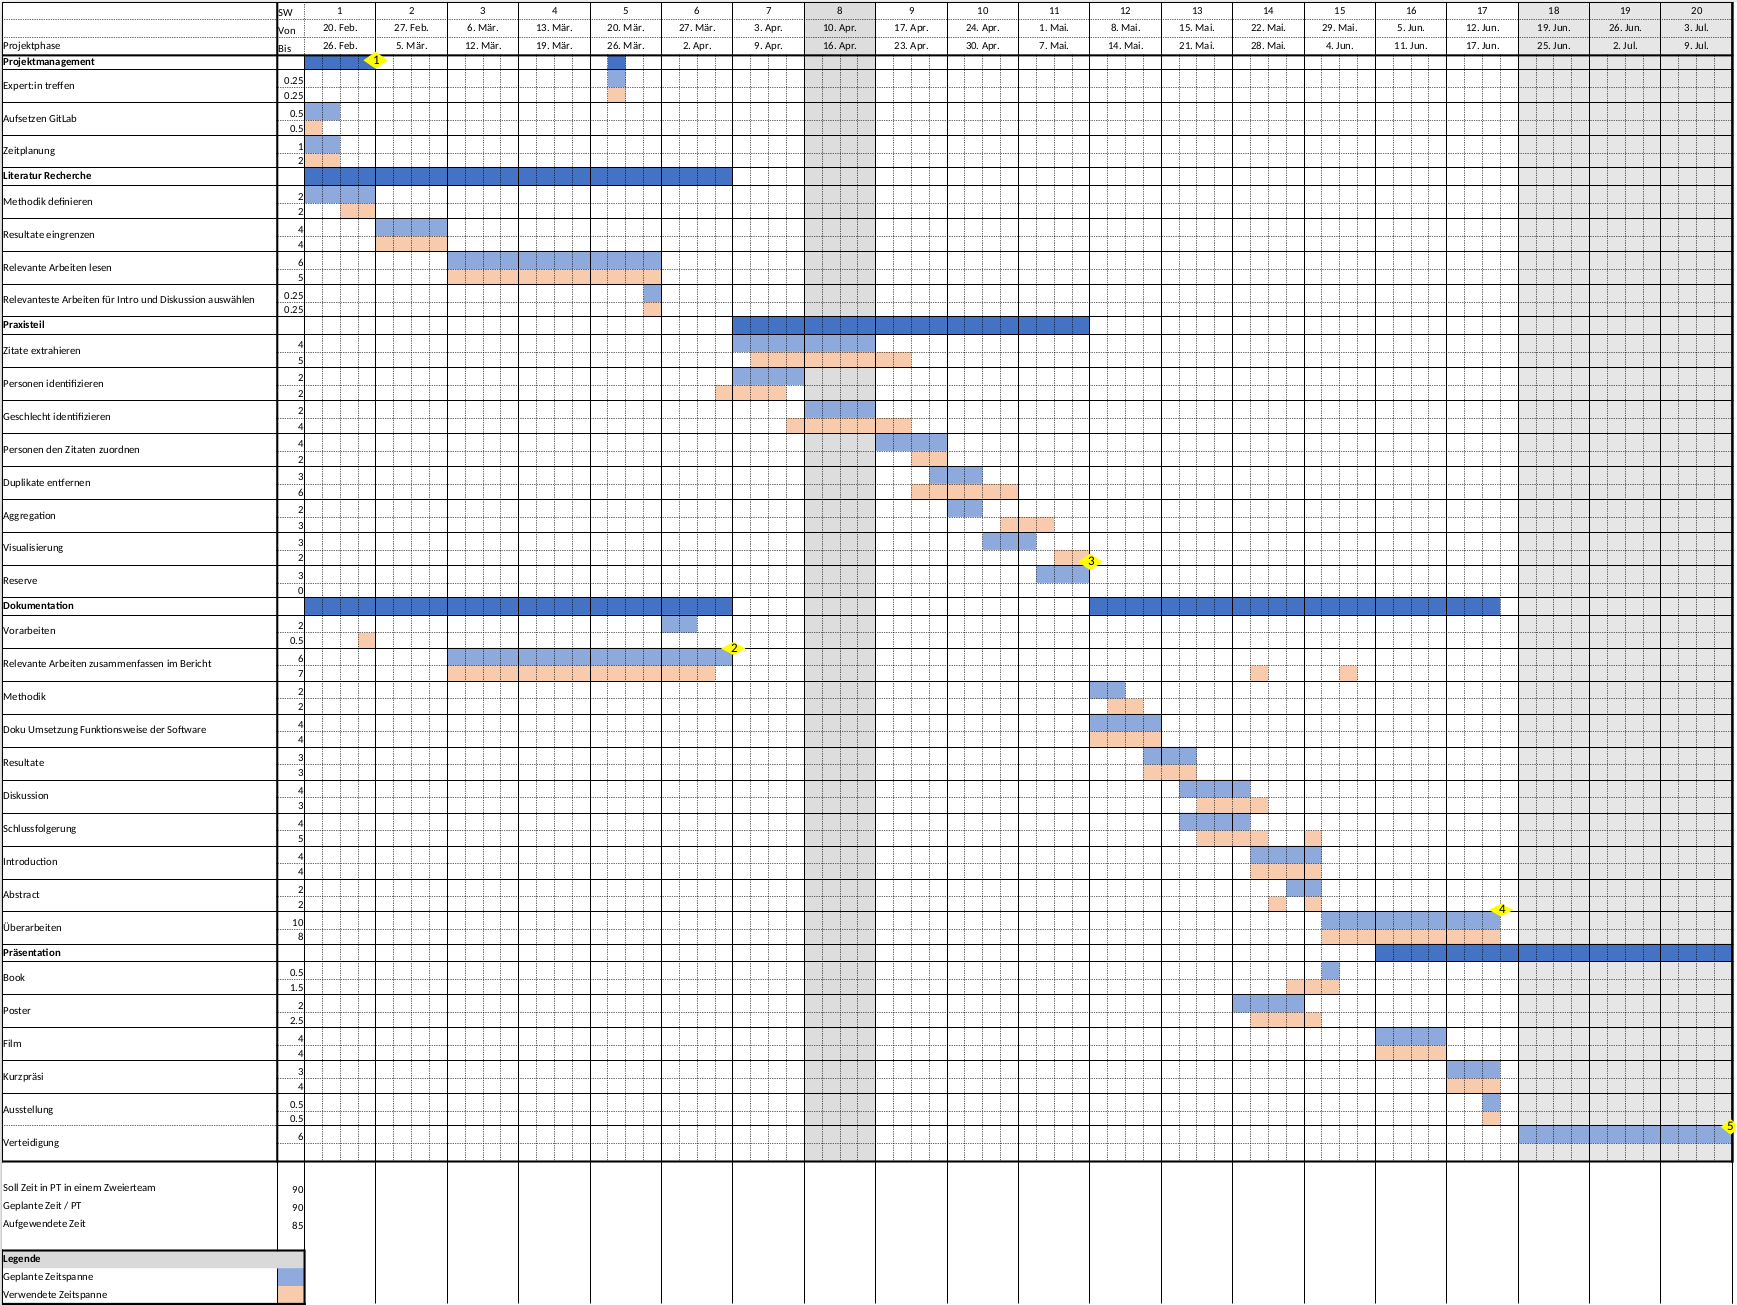
\includegraphics[width=2\linewidth,center]{images/project-planning.png}
            }}
		    \caption{Gantt Diagramm der Projektplanung}
            \label{gantt}
	    \end{center}
    \end{figure}
\newpage
% \pagenumbering{arabic}
\KOMAoptions{paper=portrait,pagesize}
\recalctypearea

\subsection{Arbeitsteilung}

Während den Besprechungen haben wir im Team die Arbeitspakete definiert und im Anschluss auf unserem
Sprint Board auf GitLab eingetragen und beschrieben. Dieses half uns, die offenen Arbeiten und Fragen
nachzuverfolgen und Doppelspurigkeiten zu Identifizieren und zu Eliminieren. Gemäss dem Projektplan haben wir
pro Projektphase ein Sprintboard erstellt, wo wir die aktuell relevanten Arbeiten stets auf einen Blick
sichtbar machen konnten. Dies half uns auch, nicht von offenen Arbeiten aus kommenden Phasen abgelenkt
zu werden. Die nachfolgende Abbildung \ref{sprint-board-screenshot} zeigt einen Screenshot vom Board der Dokumentationsphase.

\begin{figure}[H]
	\begin{center}
        \centering
		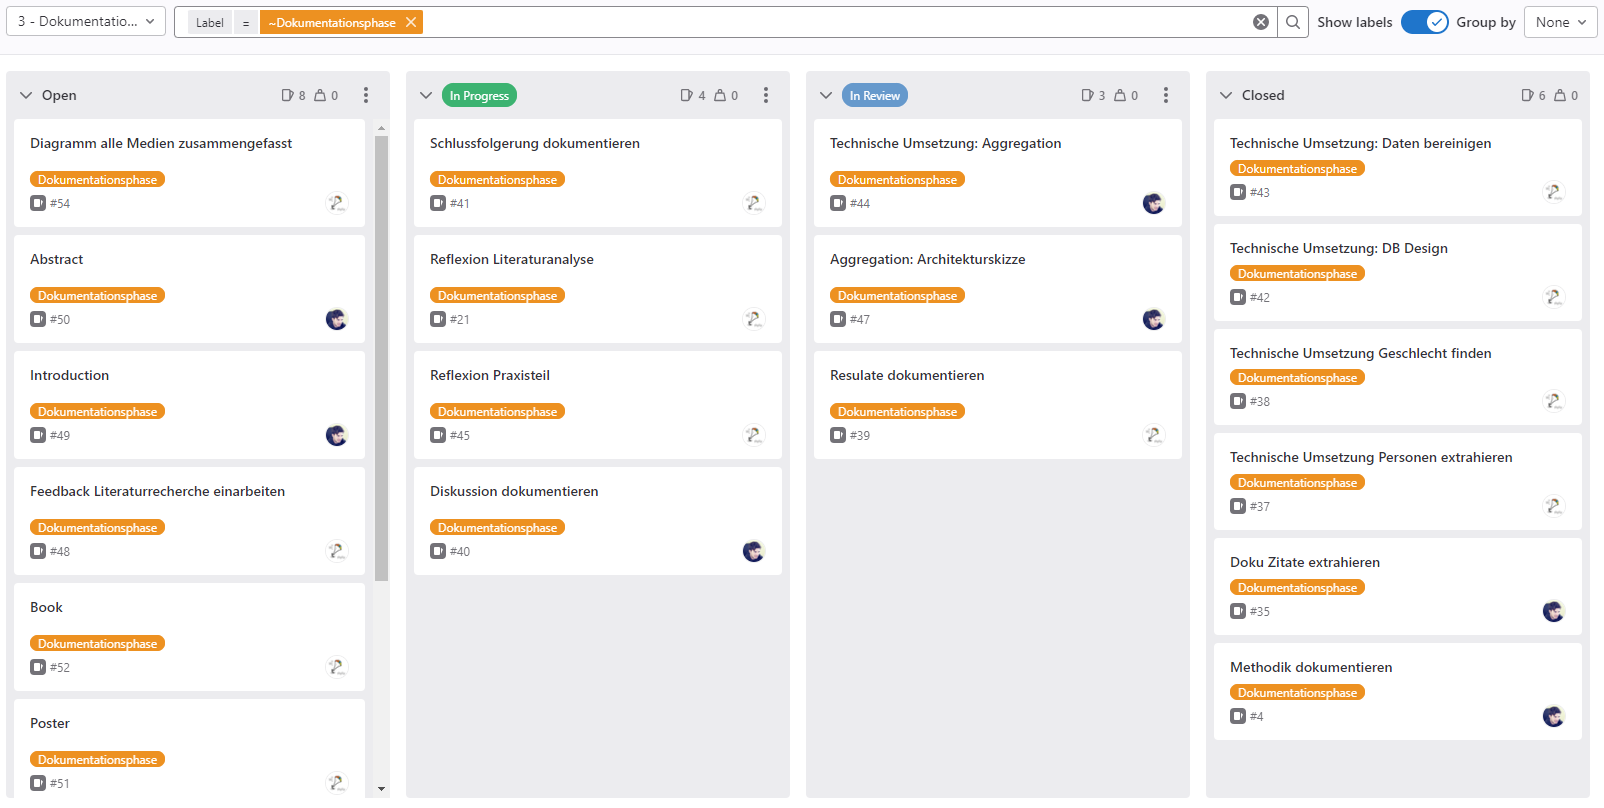
\includegraphics[width=1\linewidth]{./images/kanban_board.PNG}
		\caption{Sprint Board der Dokumentationsphase}
        \label{sprint-board-screenshot}
	\end{center}
\end{figure}

\subsection{Besprechungen}

Für die optimale Zusammenarbeit im Team waren wir stets bemüht, Entscheide gemeinsam zu fällen und
deren Ausführung im Anschluss möglichst unabhängig voneinander abschliessen zu können, um möglichst
effizient Fortschritte erzielen zu können.

Dazu trafen wir uns regelmässig am Montagabend zu einem wöchentlichen Austausch im Team, wo wir den
aktuellen Zwischenstand unserer Arbeiten, allfällige Probleme und weitere Schritte besprachen.
Zudem sahen wir uns zusätzlich stets am Freitag im Unterricht, wo wir uns informell austauschen und
neue Ideen besprechen konnten.

Zusätzlich zu den wöchentlichen Sitzungen im Kernteam trafen wir uns ungefähr jede zweite Woche mit
unserer Betreuerin, Prof. Dr. Mascha Kurpicz-Briki, um ihr den aktuellen Stand der Arbeiten und den
Fortschritt gemessen am Projektplan präsentieren zu können. In diesen Meetings konnten wir zusätzlich
inhaltliche und Formelle Fragen klären und durch Feedback von der grossen Erfahrung unserer Betreuerin
profitieren.

\section{Methoden und Konzepte zur technischen Umsetzung}

\subsection{Grundsätzliches Vorgehen}

% Einleitung + Methode P2
Das grundsätzliche Vorgehen (Methodik) wurde bereits im Vorprojekt
\cite{project2} definiert. In diesem wurden vier technische
Hauptaufgaben identifiziert, die untereinander keine oder wenige
Abhängigkeiten aufweisen. Diese resultieren in Funktionen, die auf
den gesammelten Texten oder dem Output der vorherigen Funktion operieren.
Die Abbildung \ref{dag-tasks} stellt diese Aufgaben als \gl{dag} dar.
\begin{figure}[H]
	\begin{center}
        \centering
		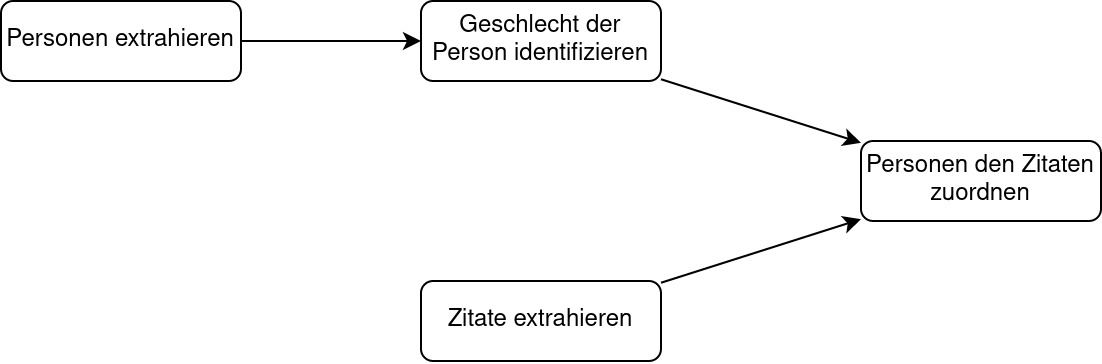
\includegraphics[width=1\linewidth]{./images/Teilaufgaben.jpg}
		\caption{\gl{dag} der Hauptaufgaben im Projekt}
		\label{dag-tasks}
	\end{center}
\end{figure}

% Zitate extrahieren
Das Extrahieren der Zitate ist von allen Teilaufgaben am unklarsten.
Teil dieser Aufgabe ist das Erkennen von eindeutigen Mustern in Zitaten
und deren Ausnutzung zur Extraktion. Der kanadische \along{ggt} (\ashort{ggt}) kann dabei
Inspiration liefern. Weil das deutsche Sprachmodell fürs \gl{dependency-parsing}
aber andere Labels verwendet als das französische und englische,
welche die Autorinnen und Autoren des kanadischen \gl{ggt} verwendet haben,
muss dieser Teil neu erfunden werden (vgl. Abschnitt \ref{citation-extraction}).

% Personen extrahieren
Die Funktion zum Extrahieren der Personen (und dazugehörigen Beschreibungen) 
wird die Software mithilfe der \gl{pos} Tagging und \gl{ner} Funktionen des \gl{spacy} Parsers umsetzen.
Die grösste Herausforderung bei dieser Aufgabe ist das \gl{cr}.
Denn für das Bestimmen des Geschlechts einer Person ist es hilfreich,
möglichst viele Aliase, Artikel und Pronomen zu kennen (vgl. Kapitel \ref{people-extraction}).

% Geschlechter bestimmen der Personen
Zum Bestimmen des Geschlechts einer Person können alle zugehörigen Informationen
verwendet werden. Am aussagekräftigsten sind Artikel und Pronomen, wobei die Zuverlässigkeit
ihrer Extraktion nicht sehr hoch ist. Ein weiteres Indiz für das Geschlecht gibt
der Vorname. Dazu wollen wir das Namensregister vom Bund zum Abfragen verwenden
\cite{bfs-vornamen-maennlich,bfs-vornamen-weiblich}. Als Backup sollen APIs aus dem
Internet dienen. Diese haben ein Rate-Limit und können nicht zu häufig abgefragt werden
(vgl. Abschnitt \ref{identify-gender}).

% Personen den Zitaten zuordnen
Als letzte Teilaufgabe gilt es, die Zitate den extrahierten Personen zuzuordnen.
Dazu wird die Position im Text und Textähnlichkeit des Namens im Zitat
und aller Eigenschaften der extrahierten Person verwendet.

% Auswertung / Aggregation
Die schlussendliche Aggregation führt für alle Artikel in der Datenbank
die bereits beschriebenen Funktionen aus und speichert das Resultat wie im 
(vgl. Kapitel \ref{db-design}).

% GG Formula
Nachdem die Software alle rund 350'000 Artikel analysiert hat, gilt es diese
auszuwerten. Das Ziel dieser Arbeit ist das Bestimmen des \gl{gendergap}s,
dem Unterschied im Raum, den Männer und Frauen in den Medien einnehmen.
Um diese klar mit einer Zahl benennen zu können, verwenden wir die abstrakte
Kennzahl \gl{gendergap} (vgl. Abschnitt \ref{ggt-formula-section}).

\subsection{Die Kennzahl \textsl{Gender Gap}}\label{ggt-formula-section}

Um den \gl{gendergap} zwischen unterschiedlichen Arbeiten vergleichen zu können,
definieren wir den \gl{gendergap} wie folgt.
Die Kennzahl repräsentiert den Unterschied im Raum, der den beiden Geschlechtern \enquote{männlich} und
\enquote{weiblich} gegeben wird, gemessen am kombinierten Anteil der Männer und Frauen.
Der \gl{gendergap} liegt deshalb stets zwischen 0 und 1,
wobei ein \gl{gendergap} von 0 eine Verteilung von 50:50 auf Männer und Frauen bedeutet
und ein \gl{gendergap} von 1 eine Verteilung des gesamten Raums auf ein Geschlecht.

Im Fall von dieser Arbeit sind mit \enquote{Raum} die Anzahl Zitate
gemeint. Die Abstraktion \enquote{Raum} ist deshalb nützlich, weil sich damit die \gl{gendergap}s
unterschiedlicher Arbeiten vergleichen lassen. So können wir beispielsweise den \gl{gendergap} des \enquote{Body Counts}
der Ringier EqualVoice Initiative \cite{ringier-equalvoice} mit unserem \gl{gendergap} anhand der
Anzahl Zitate vergleichen. Wir machen uns dies im Kapitel \ref{interpretation} zunutze, um die Ergebnisse
mit den relevantesten Arbeiten aus dem Kapitel \ref{state-of-the-art} zu vergleichen.
Keine der beigezogenen relevanten Arbeiten verfügt über eine Methodik, Formel oder Kennzahl,
mit der ein ähnlicher Vergleich möglich wäre. Die Untenstehende Formel ist ein Vorschlag,
diese Lücke zu füllen.

\begin{figure}[H]
    \begin{equation}
        Gender \, Gap = \left|\frac{RF - RM}{RF + RM}\right|
    \end{equation}
    \parbox{\linewidth}{Wobei~$RF$ der Raum ist, der Frauen gegeben wird und~$RM$ derjenige, der den Männern gegeben wird.}
    \caption{Formel zur Berechnung des \gl{gendergap}s}
    \label{ggt-formula}
\end{figure}

\subsection{Die verschiedenen Arten von Zitaten}\label{types-of-citations}

Für die Unterscheidung der Arten von Zitaten orientiert sich diese Arbeit
an der Vorbildstudie \citetitle{gender_gap_tracker} \cite{gender_gap_tracker}. Diese unterscheidet im Grundsatz
zwei Arten von Zitaten, die
\begin{enumerate}
    \item \textsl{Syntaktischen} und die
    \item \textsl{Schwimmenden Zitate}.
\end{enumerate}

Die Begründung für diese Unterscheidung ist im Kapitel \ref{ggt-method-citation} genauer
beschrieben. Was sind also \textsl{Syntaktische} und \textsl{Schwimmende} Zitate? \textsl{Syntaktische Zitate}
sind diejenigen Satzstrukturen, die alle Informationen beinhalten, die zu einem Zitat gehören:
\begin{enumerate}
    \item Ein Zitat in der direkten oder indirekten Rede
    \item Ein Subjekt, das zitiert wurde
    \item Ein Zitat-einleitendes Verb
\end{enumerate}
Ein Beispiel dafür ist \enquote{Der Bundesrat Berset versicherte, dass genügend Masken vorhanden seien.} oder \enquote{Der Bundesrat Berset versicherte: \enquote{Es sind genügend Masken vorhanden.}}.
In diesem Beispiel ist das Zitat \enquote{dass genügend Masken vorhanden seien} beziehungsweise \enquote{Es sind genügend Masken vorhanden}. Das Subjekt ist in beiden Fällen
\enquote{Der Bundesrat Berset}. Auch das einleitende Verb ist in diesen Fällen gleich, nämlich \enquote{versicherte}.

\textsl{Schwimmende Zitate} finden sich besonders in Texten, in denen eine Person mehrfach zitiert und das Subjekt nicht jedes Mal wiederholt wird.
Um beim vorherigen Beispiel zu bleiben, können wir uns eine Weiterführung des Textes so vorstellen: \enquote{Der Bundesrat Berset versicherte, dass genügend Masken vorhanden seien.
\enquote{Es sind genug für alle da.}}. Das Zitat \enquote{\enquote{Es sind genug für alle da.}} \textsl{schwimmt} im Text ohne selbst von einem Verb eingeleitet oder im selben Satz
von einem Subjekt begleitet zu werden. Für uns Menschen ist damit implizit klar, dass das Zitat zu der zuvor zitierten Person gehört.
Für einen Algorithmus sind solche impliziten Muster schwieriger zu erkennen und zu verbinden, weshalb solche \textsl{Schwimmenden Zitate} anders behandelt werden
müssen.


\subsection{Technologien}

Die folgenden Abschnitte erklären die Grundsätze der verwendeten Technologien.

\subsubsection{Python}
Die Applikation nutzt Python der Version 3.10, eine schwach typisierte 
Skriptsprache, die aufgrund ihrer Flexibilität eine schnelle Entwicklung
auch für grössere Anwendungen ermöglicht und dank ihres reichen Ökosystems
viele Verwendungsmöglichkeiten bietet. Diese Flexibilität bringt jedoch
auch gewisse Herausforderungen mit sich, wie z.B. die Abwesenheit von
Typen und Klammern, welche die
Zusammenarbeit im Team erschweren können. Aus diesem Grund wurde in
diesem Projekt für den produktiven Code der PEP8 Standard eingehalten und mit MyPy
eine Typisierung durchgesetzt. Diese beiden Eigenschaften stellen wir
durch Linting in der GitLab Pipeline (vgl. Abschnitt \ref{gitlab}) sicher.

\subsubsection{Git}
Git ist ein verteiltes Versionskontrollsystem, das bei der Verwaltung
von Quellcode und dessen Änderungen hilft. Entwickler:innen können mit
Git Änderungen an Code vornehmen, ihre Arbeit mit anderen teilen und
zusammenarbeiten. Git bietet auch Funktionen wie Branching und Merging,
um komplexe Entwicklungsaufgaben zu unterstützen. 

\subsubsection{GitLab}\label{gitlab}
GitLab ist eine Webanwendung, die auf Git aufbaut und ein umfangreiches
Set von Tools für die Zusammenarbeit an Softwareprojekten bereitstellt.
GitLab bietet Funktionen wie Projektmanagement, Issue-Tracking,
Continuous Integration / Continuous Deployment (CI/CD) und vieles mehr,
um die Entwicklung von Software zu erleichtern.

Die BFH hostet eine eigene Instanz von GitLab, auf der wir unser Repository
\footnote{https://gitlab.ti.bfh.ch/aesca4/bachelor-thesis-2023-gender-gap-tracker-schweizer-medien}
veröffentlicht haben.

In unserem Projekt haben wir GitLab Pipelines eingesetzt, um die
Codequalität mittels Linting sicherzustellen und das LaTeX Dokument
zu builden, sodass stets eine gültige Version verfügbar ist.
Die Abbildung \ref{fig:pipeline} zeigt die drei Jobs, die wir dafür verwenden.

\begin{figure}[H]
	\begin{center}
		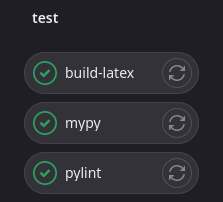
\includegraphics[width=0.5\columnwidth]{./images/gitlab-pipeline.PNG}
		\caption{GitLab Pipeline Web Crawler}
		\label{fig:pipeline}
	\end{center}
\end{figure}

\subsubsection{MongoDB}\label{mongoDB}

MongoDB ist eine dokumentenorientierte NoSQL-Datenbank, die auf flexible
Datenmodellierung und Skalierbarkeit ausgelegt ist. Im Gegensatz zu
relationalen Datenbanken verwendet MongoDB keine Tabellen, sondern
speichert Daten in Dokumenten, die in \gl{collection}s organisiert sind.
Dies ermöglicht eine einfache Handhabung von unstrukturierten Daten
und eine schnelle Abfrage von Informationen. Diese Eigenschaften
ermöglichten uns eine schnelle und flexible Entwicklung des Programmcodes.

MongoDB bietet auch ein umfangreiches Set von Funktionen wie Aggregation,
Indexierung und Volltextsuche.

Ausführlichere Informationen zu MongoDB sind auf der offiziellen Webseite
\footnote{https://www.mongodb.com/} zu finden. Zum Einbinden des Treibers
und der Verwendung mittels Python haben wir öffentlich zugängliche Tutorials
der offiziellen Seite von MongoDB\footnote{https://pymongo.readthedocs.io/en/stable/index.html}
und der Seite GeeksForGeeks \footnote{https://www.geeksforgeeks.org/python-mongodb-tutorial/} verwendet.

\subsubsection{Natural Language Processing (NLP)}

Natural Language Processing (NLP) beschäftigt sich mit der Verarbeitung
von natürlicher Sprache durch Computer und ermöglicht es, diese in eine
für Maschinen verständliche Form zu bringen. Dabei kommen
Algorithmen und Techniken zum Einsatz, die es ermöglichen, Texte zu
verstehen, zu analysieren und zu generieren. Dazu werden häufig Libraries
wie \gl{spacy} (vgl. Abschnitt \ref{spacy}) oder NLTK \footnote{https://www.nltk.org/} verwendet.

\subsubsection{Named Entity Recognition (NER)}

\gl{ner} ist eine \gl{nlp} Technologie und ermöglicht
das automatische Identifizieren von Entitäten mit Namen wie Personen,
Orten, Organisationen und Produkten in Texten. Die in diesem Projekt
geschriebene Software verwendet \gl{ner} von \gl{spacy}

\subsubsection{Part Of Speech (POS) Tagging}

\gl{pos} Tagging ist eine \gl{nlp} Funktionalität, die dazu dient, die Wortarten
(Nomen, Verb, Adjektiv...) aller Wörter in einem Satz zu bestimmen.
Im Allgemeinen werden für \gl{pos} \gl{ml} gestützte Programme verwendet,
um die Zuordnung der Wörter zu den jeweiligen Kategorien zu bestimmen.

\subsubsection{Coreference Resolution}

\gl{cr} ist eine Technik der Sprachanalyse, die darauf abzielt, Pronomen, Artikel und Synonyme im Text
auf ihre Referenz im selben Text zu beziehen. Sie identifiziert das Substantiv, auf das
sich ein Wort bezieht, um eine eindeutige Bedeutung des Satzes
zu ermöglichen. Coreference Resolution ist ein wichtiger Schritt bei der 
automatisierten Textanalyse und ermöglicht es, die Bedeutung von Texten besser zu 
verstehen. In dem Fall dieses Projekts ermöglicht die Zuordnung der Pronomen zu
den Personen eine effizientere Bestimmung des Geschlechts der Person. Da diese
zum Teil Hinweise zum Geschlecht einer Person enthalten (er, sie, sein, ihr...).

\subsubsection{Dependency Parsing}

Dependency Parsing ist eine Technik des \gl{nlp}s, die Beziehungen
zwischen Wörtern in einem Satz untersucht und hierarchisch darstellt.
Dabei wird jeder Satz in eine Baumstruktur umgewandelt, in dem jedes
Wort einen Knoten darstellt und die Beziehungen zwischen den Wörtern durch
Kanten dargestellt werden. Die Beziehungen sind abhängig von der Bedeutung
des Satzes und geben an, welches Wort mit welchem anderen Wort zusammenhängt.

\subsubsection{Spacy}\label{spacy}

\gl{spacy} ist eine Open-Source-Bibliothek für \gl{nlp}, die in Python geschrieben wurde.
Sie bietet Entwickler:innen eine Vielzahl von Funktionen zur Verarbeitung von
Texten, einschliesslich Tokenisierung, \gl{pos}-Tagging, \gl{ner} und
\gl{dependency-parsing}. Spacy wurde für hohe Leistung und Geschwindigkeit entwickelt
und ist auf die Verarbeitung grosser Textmengen ausgelegt. Die Library verfügt über Modelle,
die in mehreren Sprachen verfügbar sind und es ermöglichen, Texte in verschiedenen
Sprachen zu verarbeiten.

In unserem Projekt haben wir das Spacy Modell \enquote{de\_core\_news\_lg}
\footnote{https://spacy.io/models/de/\#de\_core\_news\_lg} verwendet, um die
Funktionen \gl{ner}, \gl{pos}-Tagging und \gl{dependency-parsing} auf deutschsprachige
Texte anzuwenden.

%\input{content/methoden/ziele-projekt.tex}

%\chapter{Hauptteil}
%The main part explains what you did in your project. The content depends on the topic of
%the project and can if necessary be split in multiple chapters. For example, you can describe
%your implementation and an experimental setup, if applicable. In other cases, a concept can
%be defined here.

\chapter{Technische Umsetzung}

Die technische Umsetzung der durchgeführten Analyse ist von der
Pipeline Architektur inspiriert. Die geschriebenen Skripts profitieren
von der isolierten Natur der Aufgabe und wenden wo immer möglich
funktionale Prinzipien wie Immutability, Higher Order- und Pure Functions
an.

Die untenstehende Abbildung \ref{flowchart-aggregation} zeigt den
grundsätzlichen Ablauf der Analyse der Daten. Dabei implementiert
die Software sowohl Aspekte des Batch- wie auch des Stream Processings.
Einerseits läuft die Auswertung von Anfang bis zum Schluss auf dem gesamten
Datensatz durch, andererseits nutzt sie einen MongoDB Cursor, der die
Artikel aus der DB Stück für Stück herunterlädt (streamt). Dieser Cursor ermöglicht
es dem Programm, bereits heruntergeladene Artikel zu analysieren und nach
Abschluss wieder aus dem Speicher zu löschen, um Ressourcen zu schonen.
Des Weiteren verwendet das Skript einen Processor Pool, der die gleichmässige
Verteilung der Last auf alle CPU Kerne garantiert und damit die zur Verfügung
stehenden Ressourcen ganz ausnutzt.

\begin{figure}[H]
	\begin{center}
        \centering
		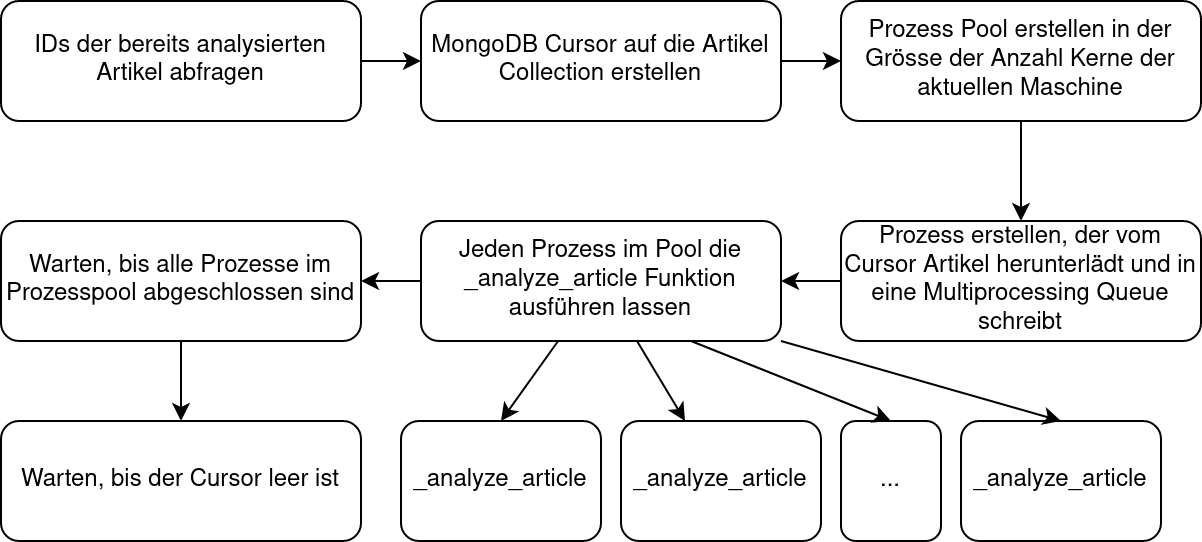
\includegraphics[width=1\linewidth]{./images/aggregate.png}
	\end{center}
	\caption{Ablaufdiagramm der Auswertung}
	\label{flowchart-aggregation}
\end{figure}

Die Abbildung \ref{aggregation-function} zeigt den Python Code,
der über den Prozessor Pool auf die einzelnen CPU Kerne verteilt wird.
Diese Funktion konsumiert Artikel aus der \enquote{articles\_queue},
einer Multiprocessing-sicheren Datenstruktur, die nach und nach vom
MongoDB Cursor mit Artikeln aus der DB gefüllt wird.
Die Funktion läuft so lange, bis sie für mindestens zehn Minuten
keine neuen Artikel in der Queue mehr findet. Der Grund für dieses eher hohe
Timeout sind mögliche Netzwerkprobleme oder andere unvorhergesehene
Unterbrüche. Bei Verarbeitung solch grosser Datenmengen fallen die
zusätzlichen 10 Minuten nicht ins Gewicht und sind betreffend
Performanz zu vernachlässigen.
Nach dem Erhalt eines neuen Artikels bestimmt der Algorithmus,
ob der aktuelle Artikel bereits analysiert wurde.
Falls ja, verwirft er ihn wieder und holt sich einen neuen.
Danach beginnt die effektive Analyse. Einzelne Funktionen daraus sind
in den nachfolgenden Kapiteln näher beschrieben.
Als nächstes bestimmt die Funktion das Geschlecht des Autors, danach durchsucht
sie den Text nach Personen und Zitaten. Zum Schluss weist sie
die gefundenen Personen den gefundenen Zitaten zu und speichert das
Resultat in der Datenbank.
Wenn die Abfrage der Queue in ein Timeout läuft (zehn Minuten), dann
wirf die Funktion eine \enquote{Empty} Exception, die vom \enquote{except}
Block abgefangen wird und dazu führt, dass die Funktion und damit der
Prozess beendet wird.

\begin{figure}[H]
    \begin{lstlisting}[language=Python]
def _analyze_article(processor_nr: int) -> None:
    log.info("Starting processor %d", processor_nr)
    while True:
        try:
            article_dict = articles_queue.get(
                timeout=600
            )  # 10min, in case of network issues

            if article_dict["_id"] in analyzed_articles:
                continue

            builder = ArticleBuilder()
            article = builder.from_db_result(article_dict).build()

            genderized_author = get_genderized_person(
                get_person_from_string(article["author"])
            )

            article_text = article["text"]
            people = get_people_from_string(article_text)
            genderized_people = map(get_genderized_person, people)

            citations = get_syntactic_quotes(article_text)
            citations_with_person = assign_people_to_citations(
                genderized_people, citations
            )

            analyzed_article = get_analyzed_article(
                article, genderized_author, citations_with_person
            )
            insert_analyzed_article(analyzed_article)

        except Empty:
            log.info("Queue is empty! Terminating processor %d!", processor_nr)
            return
    \end{lstlisting}
    \caption{Funktion: \_analyze\_article()}
    \label{aggregation-function}
\end{figure}

\newpage
\section{Datensammlung bereinigen}

Die Vorarbeit hat eine Datensammlung von etwa 370'000 Nachrichtenartikeln ergeben, die jeweils über eine eindeutige URL verfügen. 
Wir haben durch die Verwendung von Unique Constraints sichergestellt, dass jede URL einzigartig ist. 
Allerdings vermuteten wir, dass die Datensammlung Duplikate von Texten enthält, die unter verschiedenen URLs veröffentlicht wurden. 
Dies könnte durch Weiterleitungen auf andere Seiten oder veränderte URLs verursacht worden sein. 
Um eine genaue Aussage über den Gender Gap in diesen Nachrichtenportalen machen zu können, mussten wir alle Duplikate pro Nachrichtenportal eliminieren. 

Nach einigen Testversuchen mit 1000 Artikeln entschieden wir uns dafür, die \gl{cosine-similarity} zu verwenden, um Artikeltexte untereinander zu vergleichen. 
Dieser Vergleich war bei den Tests performanter als die \gl{levenshtein-similarity}, die ebenfalls zur Auswahl stand. 
Der Rechenaufwand für den Vergleich zweier Zeichenketten der Länge m bzw. n ist bei der \gl{levenshtein-similarity} 
\(O(m*n)\), während er bei der \gl{cosine-similarity} nur \(O(m+n)\) beträgt
\footnote{https://pypi.org/project/strsimpy/}.

Die \gl{cosine-similarity} ist eine Metrik zur Messung der Ähnlichkeit zwischen zwei Vektoren.
Sie definiert die Ähnlichkeit zwischen zwei Vektoren als den Kosinus des Winkels zwischen ihnen.
In unserem Fall sind die Vektoren die Artikeltexte repräsentiert im Vector Space Modell. 
Um die Ähnlichkeit zwischen einem Vektor und einer Menge von anderen Vektoren zu berechnen, erstellen wir eine Ähnlichkeitsmatrix. 
Wenn der Kosinus 1 ist, sind die Texte gleich. 
Als Schwellwert für die Ähnlichkeit haben wir 0.9 festgelegt, da dieser bei unseren Tests am besten funktionierte. 
Wenn wir einen höheren Schwellwert genommen hätten, hätten wir nicht alle Duplikate gefunden und bei einem zu niedrigen Schwellwert
hätten wir zu viele Texte als Duplikate interpretiert, die gar keine sind. 

Da jeder Artikeltext mit jedem anderen verglichen werden muss, hätte der Algorithmus eine Matrix in der Grösse 
von 371'653 x 371'653 erstellen müssen und 42,9 GB Arbeitsspeicher benötigt. 
Das war für unsere Arbeitsmaschinen zu viel. 
Daher haben wir das \enquote{divide and conquer} Verfahren angewendet und aus einem grossen Problem kleine Teilprobleme gemacht. 
Für jeden Artikel, den wir verglichen haben, haben wir eine neue Matrix erstellt, sodass sie nur noch 1x371'653 gross war und dann nacheinander 371'653 Mal verglichen wurde. 
Wir gingen damit einen Tradeoff ein, der die Ausführungszeit verlängerte, die der Algorithmus benötigte. Das erstellte Skript benötigte zwei Tage um alle Duplikate zu finden.

Auf diese weise konnten wir alle Duplikate und nahezu-Duplikate aus der Datenbank entfernen.
Die Abbildung \ref{duplicates} gibt einen Überblick über die entfernten Artikel pro Nachrichtenportal.

\begin{figure}[H]
	\begin{center}
        \centering
		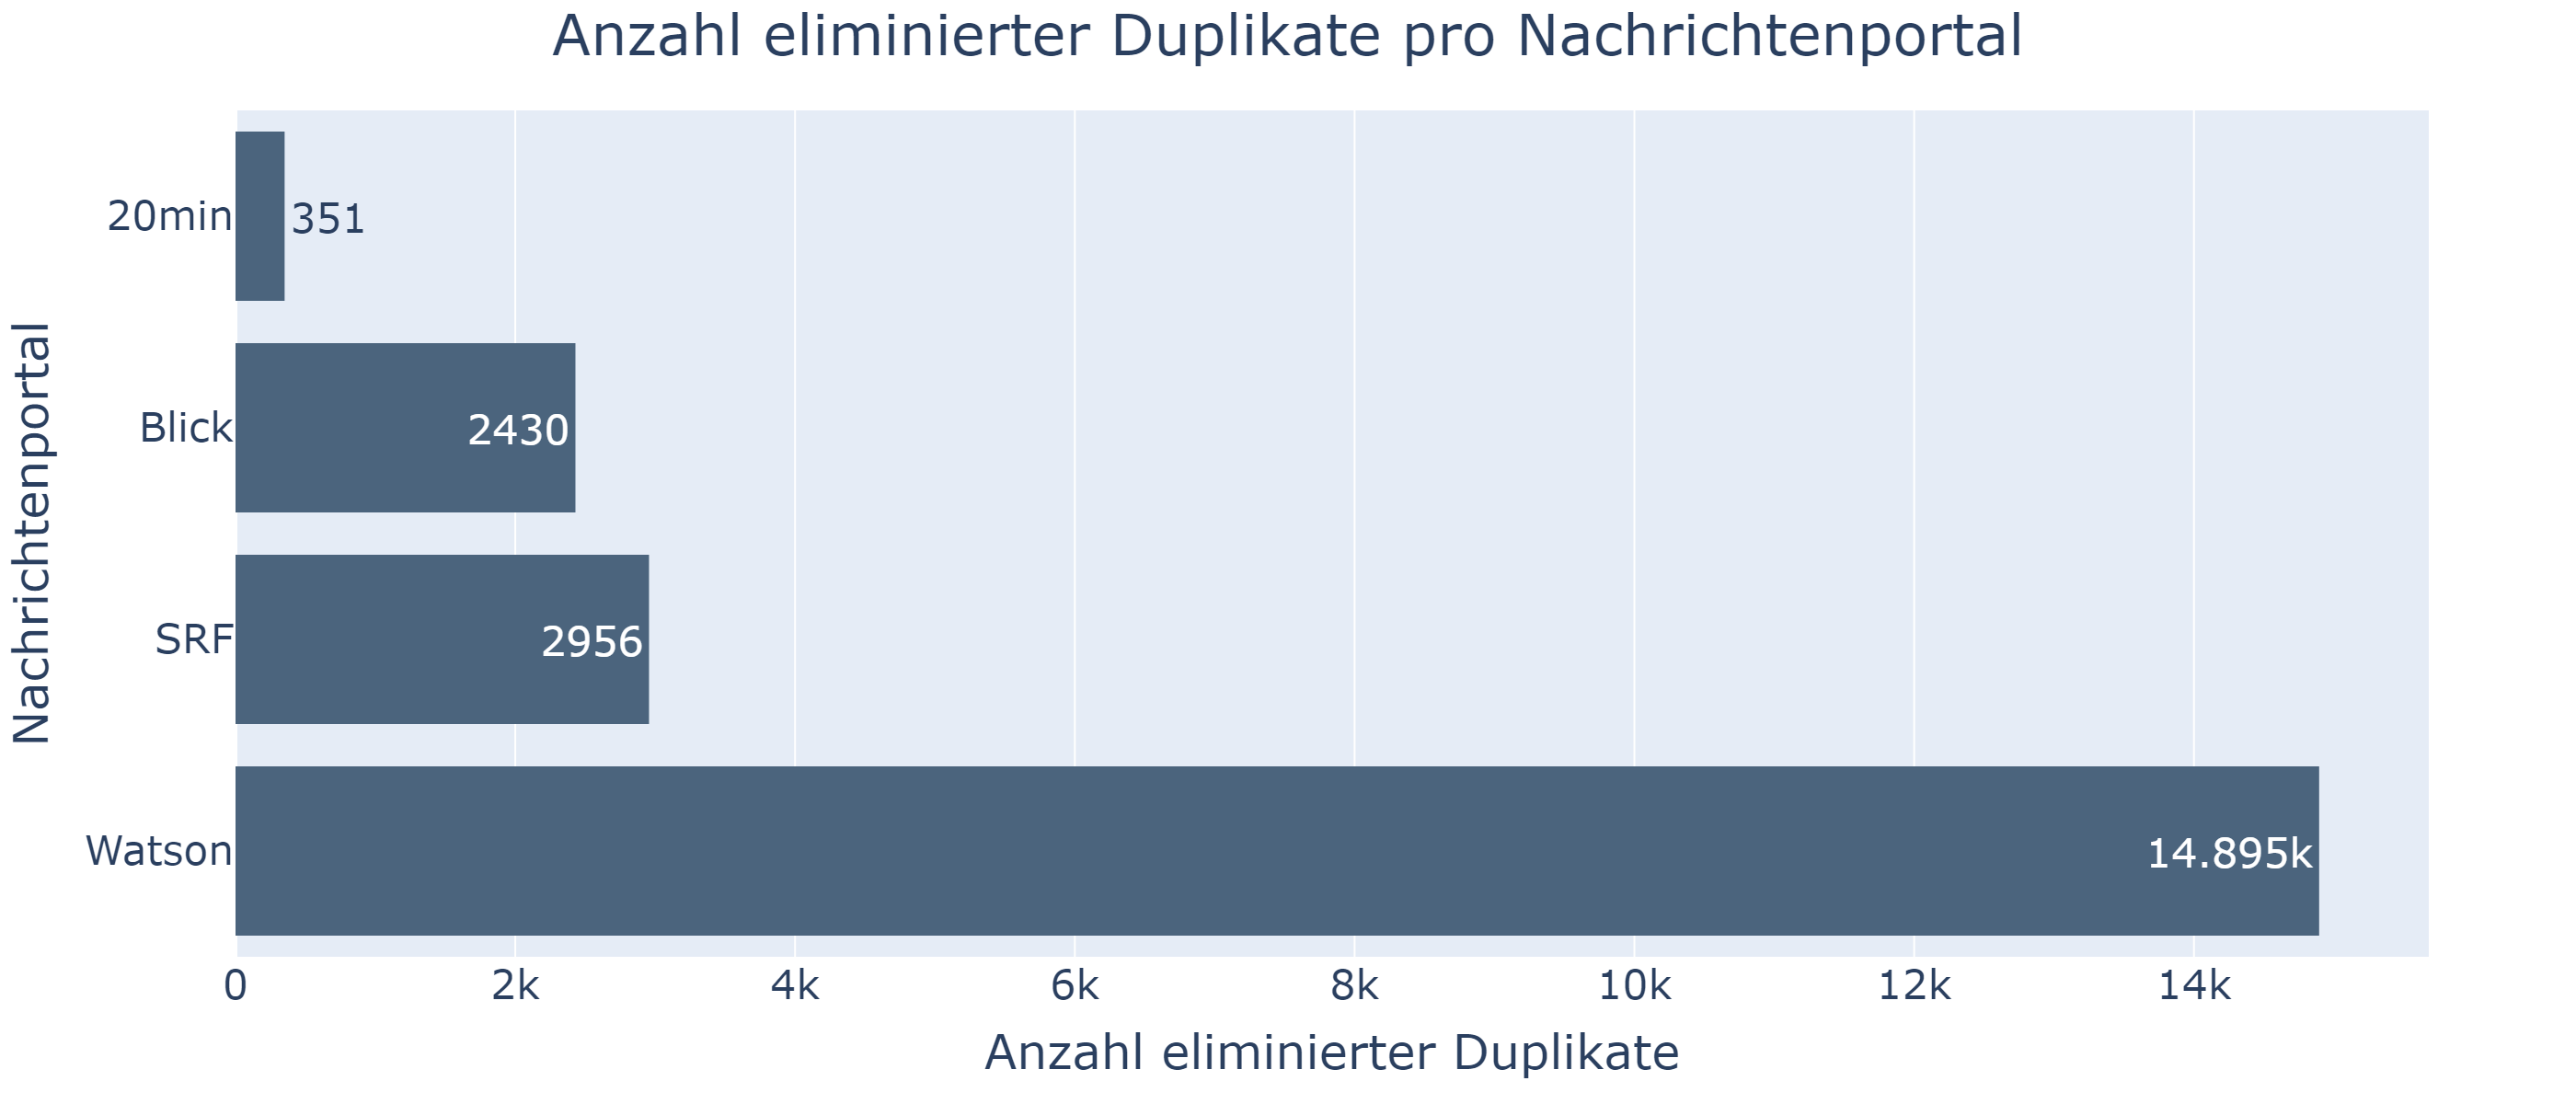
\includegraphics[width=1\linewidth]{./images/duplicates_count.png}
		\caption{Anzahl eliminierter Duplikate pro Nachrichtenportal}
		\label{duplicates}
	\end{center}
\end{figure}

\newpage
\section{Datenbank}\label{db-design}
Wir haben im Vorprojekt von der BFH eine virtuelle Maschine gemietet, auf die wir über \ashort{ssh} zugreifen können.
Auf dieser haben wir eine MongoDB installiert, um dort die Artikel zu speichern.
Die \gl{collection} \enquote{analyzed\_articles} enthält die analysierten Artikel.
Diese enthalten die gefundenen Zitate mit Personen und deren Geschlecht.
Die Struktur der Einträge ist in Abbildung \ref{structure-analyzed-articles} ersichtlich.
Darunter in der Abbildung \ref{analyzed-article} folgt ein Eintrag der DB als Beispiel.

% \newlist{myEnumerate}{itemize}{3}
% \setlist[myEnumerate]{nosep,label=\protect\mpbullet}
% \setlistdepth{6}
\begin{figure}[H]
\textbf{analyze\_articles}
\begin{itemize}
    \item \textbf{title:} Titel des Artikels
    \item \textbf{lead:} Lead Text des Artikels
    \item \textbf{url:} \ashort{url} zum Artikel, eindeutiger Schlüssel
    \item \textbf{author:} Autor:in des Artikels
    \item \textbf{source:} Das Nachrichtenportal
    \item \textbf{published:} Timestamp der Veröffentlichung
    \item \textbf{updated:} Timestamp der letzten Aktualisierung
    \item \textbf{text:} Text des Artikels
    \item \textbf{quotes:} Zitate in Form von Liste
    \begin{itemize}
        \item \textbf{designation:} Person von Zitat
        \item \textbf{gender:} Geschlecht der Person
        \item \textbf{quotation verb:} Verb welches zum Zitat einleitet
        \item \textbf{quote:} Zitat Text
        \item \textbf{start of quote in text:} Start Position von Zitat im Text
    \end{itemize}
\end{itemize}
\caption{Struktur eines Eintrags in der MongoDB Collection \enquote{analyzed\_articles}}
\label{structure-analyzed-articles}
\end{figure}

\newpage

\begin{figure}[H]
	\begin{lstlisting}
{
    "_id": "794aceeeea0911eda58075d660e6a249",
    "article": {
        "_id": "cf49cff695fa11ed8a280242ac110002",
        "title": "Nimm dich nicht zu wichtig!",
        "lead": "Bescheidenheit ist eine Zier, doch weiter kommt man ohne ihr, besagt ein Sprichwort. Doch zahlt sich Bescheidenheit wirklich weniger aus als Selbstdarstellung? Eine Bestandesaufnahme.",
        "author": {
            "designation": "Raphael Zehnder",
            "gender": "male"
        },
        "source": "srf",
        "url": "www.srf.ch/kultur/gesellschaft-religion/wochenende-gesellschaft/
        bonus-bescheidenheit-nimm-dich-nicht-zu-wichtig",
        "published": 1577005620,
        "updated": 1577005620,
        "text": "Egozentrische Pfauen tummeln sich allenthalben: Wirtschaftskapitäne blasen sich auf, Politikerinnen und Politiker lobpreisen ..."
    },
    "quotes": [
        {
            "subject": {
                "designation": "Walter Slezak",
                "gender": "male"
            },
            "quotation_verb": "brachte",
            "quote": "Wir kaufen Dinge, die wir nicht brauchen, um Menschen zu beeindrucken, die wir nicht mögen",
            "start_of_quote_in_text": 555
        }
    ]
}
        
	\end{lstlisting}
	\caption{\enquote{analyzed\_articles} \gl{collection} Eintrag Beispiel}
	\label{analyzed-article}
\end{figure}

\newpage
\section{Personen extrahieren}\label{people-extraction}

% 1. NER Entitäten mit Personen Tag aus Text lesen
% 2. Mit Coreference resolution Personen Cluster bekommen
% 3. NER Coreference und Coref-Res Entitäten verbinden um eindeutige Personen zu bekommen mithilfe der Schnittmenge der Wörter
% Dabei wird aus den Coreference Einträge neben Vornamen und Nachnamen der Person auch noch Pronomen und Artikel herausgelesen mit POS und der Person zugewiesen.
% diese sind dann zusätzlich zum Vornamen hilfreich für das Geschlecht der Person zu bestimmen.

Das Extrahieren von Personen aus einem Text umfasst mehrere Schritte.
Zunächst werden die Entitäten mit dem Tag \enquote{Person} mithilfe von \gl{ner} aus dem Text herausgelesen.
Als Nächstes wird \gl{cr} verwendet, um Personencluster zu bilden. 
Dies bedeutet, dass der Text auf Referenzen zu Personen überprüft wird, z.B. wenn eine Person im Text als \enquote{sie} oder \enquote{er} bezeichnet wird. 
\gl{cr} hilft dabei, alle Referenzen auf dieselbe Person zu identifizieren und in Gruppen zu organisieren.
Um eindeutige Personen zu erhalten, müssen die NER-Entitäten und die Coreference-Entitäten zusammengeführt werden.

Dazu werden die Schnittmengen der Wörter verwendet, die den NER- und Coreference-Entitäten zugeordnet sind.
Auf diese Weise können Personen und zugehörige Informationen eindeutig identifiziert werden.
Zusätzlich zu den Vornamen und Nachnamen der Person werden auch Pronomen und Artikel, die mit der Person in Verbindung stehen aus der Coreference-Entität, mithilfe von \gl{pos} 
extrahiert und der Person der pronouns\_and\_articles Liste zugewiesen. 
Damit die Zuordnung von den Zitaten zu den Personen im nächsten Schritt einfacher ist, speichern wir die Positionen im Text wo die Personen genannt wurde auch ab unter dem positions\_in\_text Attribut der Person Klasse.
Weil \gl{ner} Entitäten zusätzlich zum Namen auch Titel wie \enquote{Prinz} oder \enquote{Herzogin} haben können, 
wurden diese mithilfe einer eigens definierten Liste erkannt und unter dem substitute\_nouns Attribut abgelegt. 
All das wird in der Funktion \_\_get\_people\_from\_ner\_coref (vgl. Abbildung\ref{get-people-from-ner-coref}) gemacht, welche als Input eine Liste der \gl{ner} und \gl{cr} Entitäten bekommt.
Die zusätzlichen Informationen, welche der Algorithmus mittels der Coreference-Entität zur Person erhält, sind im nächsten Schritt hilfreich, um das Geschlecht der Person zu bestimmen.
Der Rückgabewert der Funktion ist eine Liste von \textsl{Person} Objekten. Diese Klasse ist in der Abbildung \ref{person-class} ersichtlich.

\begin{figure}[H]
    \begin{lstlisting}[language=Python]
        def __get_people_from_ner_coref(
            ner_people_list: List[Tuple[List[str], List[int]]], 
            coref_list: List[str]
        ) -> List[Person]:
            """
            This method creates people with the help of the NER list and the coref list
            """
            people = []
        
            for person_words in ner_people_list:
                new_person = Person("", "", [], [], [], [])
                for person_word in person_words[0]:
                    for coref_entry in coref_list:
                        if person_word.lower() in coref_entry:
                            pos_res = nlp(coref_entry)
                            for word in pos_res:
                                if word.pos_ == "PRON":
                                    new_person.pronouns_and_articles.append(word.text)
                                if word.pos_ == "DET":
                                    new_person.pronouns_and_articles.append(word.text)
                                if word.pos_ == "NOUN":
                                    new_person.substitute_nouns.append(word.text)
        
                # handle substitute nouns
                # z.B. wenn NER Eintrag Prinz Harry ist, dann wird Prinz zu substitute_nouns Liste der Person hinzugefügt
                person_name = __handle_substitute_nouns(new_person, person_words[0])
        
                # wenn keine Namen sondern nur substitute_nouns gefunden,
                #  dann wird neue Person nicht liste hinzugefügt
                if len(person_name) > 0:
                    new_person.first_name = person_name[0]
                    if len(person_name) > 1:
                        # um Nachnamen wie "Le Clos" oder "Von Niederhaeusern" zu erkennen
                        last_name = " ".join(person_name[1:])
                        new_person.last_name = last_name
        
                    new_person.positions_in_text = person_words[1]
        
                    people.append(new_person)
        
            return people        
    \end{lstlisting}
    \caption{Function \_\_get\_people\_from\_ner\_coref}
    \label{get-people-from-ner-coref}
\end{figure}

\begin{figure}[H]
	\begin{lstlisting}[language=Python]
    class Person:
        first_name: str
        last_name: str
        pronouns_and_articles: list[str]  # z.B.: er, sie, ihr, ihre, sein, seine der, die, das
        substitute_nouns: list[str]  # z.B.: Informatikerin, Studentin, Schwester, Tochter, Prinz, Experte
        positions_in_text: list[int]
	\end{lstlisting}
	\caption{Person Klasse}
	\label{person-class}
\end{figure}

\section{Geschlecht identifizieren}\label{identify-gender}

% Liste Vornamen Bund 2021
% Pronemen Listen
% Genderzie API

Um das Geschlecht einer Person herauszufinden, werden als Erstes die offiziellen Listen 
\footnote{https://www.bfs.admin.ch/bfs/de/home/statistiken/bevoelkerung/geburten-todesfaelle/namen-schweiz.html} 
von Vornamen aus dem Jahr 2021 des Bundesamts für Statistik konsultiert. 
Davon gibt es zwei, eine mit männlichen und eine mit weiblichen Vornamen.
Dann werden die Pronomen der Person, falls vorhanden, verglichen, ob sie wahrscheinlicher männlich oder weiblich sind.
Wenn die Wahrscheinlichkeit aus den Pronomen und der Liste vom Bundesamts für Statistik unter 66\% liegt, dass es zum einten Geschlecht gehört,
wird die API von Genderize.io mit dem Vornamen abgefragt. Bei dieser API gibt es jedoch eine Begrenzung von 1000 Requests pro Tag.
Wenn dieses Limit erreicht ist, wird trotzdem das wahrscheinlichere Geschlecht aus dem Resultat der Liste vom Bundesamts für Statistik und den Pronomen gewählt.
Das Geschlecht der Person wird dann in der Form eines \textsl{Gender} Enums (vgl. Abbildung \ref{genderized-person-class}) zurückgegeben.

\begin{figure}[H]
	\begin{lstlisting}[language=Python]
    class GenderizedPerson(Person):
        gender: Optional[Gender]  # Unknown => None
        probability: float
    
    class Gender(Enum):
        UNKNOWN = 0
        FEMALE = 1
        MALE = 2        
	\end{lstlisting}
	\caption{GenderizedPerson Klasse und Gender Enum}
	\label{genderized-person-class}
\end{figure}


\newpage
\section{Extraktion der Zitate}\label{citation-extraction}

Die vorliegende Auswertung bezüglich der Anzahl Zitate von Männern und Frauen pro Nachrichtenportal
fokussiert sich auf das Erkennen und Extrahieren der sogenannten \textsl{Syntaktischen Zitate}.
Der Grund dafür ist, dass diese von der Form her die klarste Struktur aufweisen und auch die Basis
für das Erkennen der anderen Arten von Zitaten darstellen.

Weitere Arten von Zitaten, die in dieser Arbeit aufgrund des zeitlichen Rahmens nicht berücksichtigt
werden konnten sind
\begin{enumerate}
    \item \textsl{Schwimmende Zitate},
    \item \textsl{Heuristische Zitate} und
    \item \textsl{Syntaktische Zitate}, die ein zu unspezifisches oder gar kein Verb enthalten.
Das können Zitate sein, die mit \enquote{gemäss} oder \enquote{so} usw. eingeleitet werden.
\end{enumerate}

Nachfolgend ist deshalb ausschliesslich die Extraktion der \textsl{Syntaktischen Zitate} mit spezifischen
Verben beschrieben. Auf die weiteren Arten und deren mögliche Erkennung wird im Kapitel
\ref{further-research} eingegangen.

Die \textsl{Syntaktischen Zitate} zeichnen sich in der Textanalyse mit \gl{spacy-parser} 
dadurch aus, dass sie im resultierenden Parse Tree in einer fast eindeutigen Struktur auftauchen
und deshalb mit einem klar definierten Regelwerk extrahiert werden können. Beispiele dazu finden sich
in den nachfolgenden Unterkapiteln.

\subsection{Parse Trees}

Die Analyse eines Texts (Strings) mit dem \gl{spacy-parser} resultiert in einer Baumstruktur,
welche die Abhängigkeit der Wörter untereinander enthält. Die Aufgabe des Programms besteht also
darin, Subtrees einer gewissen Struktur zu erkennen. Die Abbildung \ref{tree-general} ist eine
Abstraktion eines solchen Subtrees.

In den eckigen Klammern ist die Art des Worts beschrieben. Diese wird gefolgt von einem Bodenstrich (\_)
und der \gl{spacy} -Abkürzung für die Kategorie des Worts.



\begin{figure}[H]
	\begin{center}
        \centering
		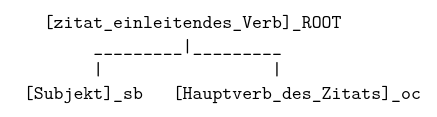
\includegraphics[width=0.6\linewidth]{./images/structure_citation.png}
	\end{center}
\caption{Subtree Repräsentation eines Syntaktischen Zitats}
\label{tree-general}
\end{figure}

Die möglichen Kategorien sind in der Tabelle \ref{legend-spacy-parsers} beschrieben. Diese Kategorien
widerspiegeln nicht konsequent Wortarten oder Begriffe aus der Satzlehre, wie sie im Deutschunterricht
gelehrt werden. Deshalb ist auch mit der Erklärung oft nicht klar, wofür sie stehen. Deren Auftreten
ist jedoch konsistent genug, sodass sie zur Erkennung der gewünschten Satzstrukturen genutzt werden
können.

\begin{table}[H]
    \centering
    \begin{tabular}{|l|r|}
        \hline
        \textbf{Spacy Parser Label} & \textbf{Spacy Erklärung} \\
        \hline
        \hline
        ROOT & root \\
        \hline
        da & dative \\
        \hline
        mnr & postnominal modifier \\
        \hline
        mo & modifier \\
        \hline
        nk & noun kernel element \\
        \hline
        oc & clausal object \\
        \hline
        punct & punctuation \\
        \hline
        sb & subject \\
        \hline
    \end{tabular}
    \caption{Legende zu den wichtigsten Spacy Parser Labels}
    \label{legend-spacy-parsers}
\end{table}

Die nachfolgenden Abbildungen \ref{tree-direct} und \ref{tree-indirect} sind konkrete Beispiele solcher
Trees. Der \gl{spacy-parser}  überrascht mit seiner Fähigkeit, Zitate in der direkten und
indirekten Rede gleich strukturieren zu können.

Die Abbildung \ref{tree-direct} repräsentiert den Satz
\enquote{Macron sagte zu Xi, »Die Aggression hat der Stabilität einen Schlag versetzt«.}
mit einem Zitat in der direkten Rede.

\begin{figure}[H]
	\begin{center}
        \centering
		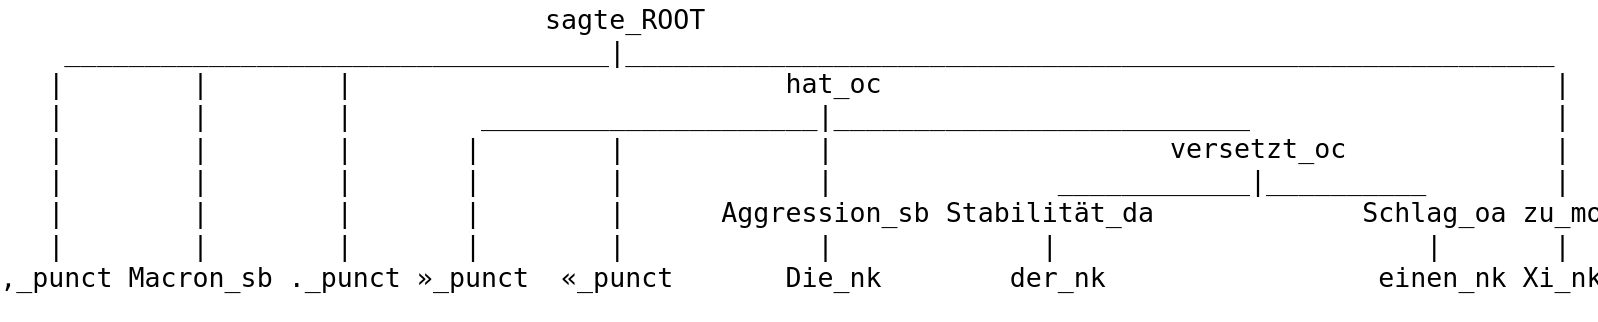
\includegraphics[width=\linewidth]{./images/macron-sagte-zu-xi-direkt.png}
	\end{center}
\caption{Parse Tree eines Satzes mit einem Syntaktischem Zitat in der direkten Rede}
\label{tree-direct}
\end{figure}

Die Abbildung \ref{tree-indirect} repräsentiert den Satz
\enquote{Macron sagte zu Xi dass die Aggression der Stabilität einen Schlag versetzt habe.}
mit einem Zitat in der indirekten Rede.

\begin{figure}[H]
	\begin{center}
        \centering
		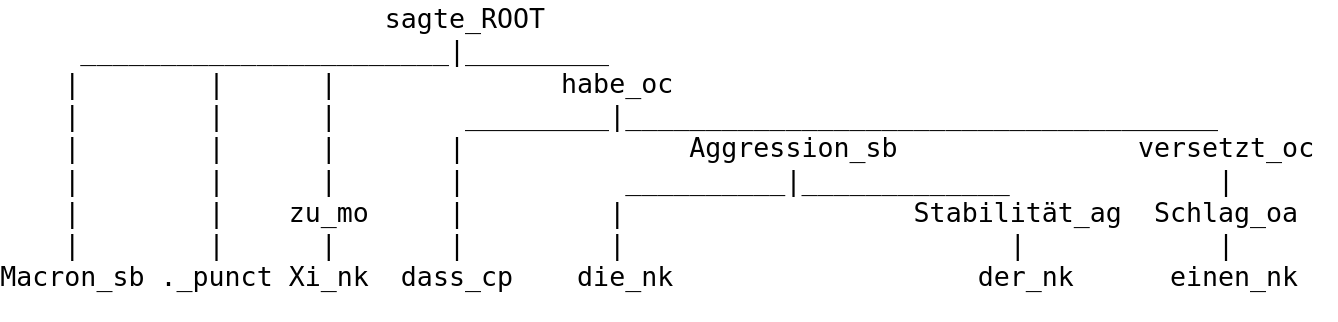
\includegraphics[width=\linewidth]{./images/macron-sagte-zu-xi-indirekt.png}
	\end{center}
\caption{Parse Tree eines Satzes mit einem Syntaktischem Zitat in der indirekten Rede.}
\label{tree-indirect}
\end{figure}

\subsection{Ablauf des Algorithmus}

Der nachfolgende Abschnitt soll konzeptuell und mit einigen Code-Beispielen erklären, wie der
Algorithmus vorgeht, um die Zitate in der oben beschriebenen Struktur zu Erkennen und zu extrahieren.

Hinweis: Im nachfolgenden Text werden die Terme \enquote{Node}, \enquote{Knoten} und \enquote{Token} als Synonyme verwendet.
Der Grund dafür ist, dass \enquote{Token} die Namensgebung von \gl{spacy}  ist und \enquote{Node} und \enquote{Knoten}
die passenden Begriffe dazu aus der Graphentheorie sind.

Der nachfolgende Code in Abbildung \ref{get-quotation-node} zeigt die Funktion, die das Programm verwendet,
um den \enquote{Hauptverb des Zitats} (vgl. Abbildung \ref{tree-general})
aus dem Parse Tree zu extrahieren. Gemeint ist damit derjenige Knoten, der als Kinder alle Wörter 
des Zitats enthält. Grundsätzlich muss die Funktion dabei unterscheiden, ob der vorliegende Satz 
in einer Zeitform mit Hilfsverb vorliegt (Perfekt, Plusquamperfekt oder Futur) oder in einer 
Zeitform ohne (Präsens oder Präteritum).

Die Funktion bedient sich einer weiteren Funktion \enquote{\_\_get\_nearest\_token\_by\_condition}
(vgl. Abbildung \ref{get-token-by-condition}), um in einer Breitensuche nach dem entsprechenden Node zu suchen.

\begin{figure}[H]
    \begin{lstlisting}[language=Python]
def __get_quote_node(root: Token) -> Token:
    result = []

    # Perfekt, Plusquamperfekt, Futur
    if root.lemma_ in __get_hilfsverben():
        condition = (
            lambda n: n.head.lemma_ in __get_quotation_verbs() and n.dep_ == "oc"
        )
        result = __get_flattened_list(
            [__get_nearest_tokens_by_condition(c, condition) for c in root.children]
        )

    # Präsens, Präteritum
    if root.lemma_ in __get_quotation_verbs():
        result = [x for x in root.children if x.dep_ == "oc"]

    if len(result) < 1:
        raise _NotFoundError()

    return result[0]
    \end{lstlisting}
    \caption{Function \_\_get\_quote\_node}
    \label{get-quotation-node}
\end{figure}

Die Funktion \enquote{\_\_get\_nearest\_token\_by\_condition} in der Abbildung \ref{get-token-by-condition} wird vom Algorithmus verwendet,
um die Knoten des Subjekts, des Zitat-einleitenden Verbes und des Zitats zu finden. Die Funktion
durchsucht den gegebenen Subtree mit der Strategie der Breitensuche, um den nächsten Knoten im Baum zu finden,
der eine vorgegebene Bedingung erfüllt. Die Bedingung ist dabei jeweils spezifisch für den gesuchten Knotentyp.

Das Resultat ist derjenige Knoten, der den kürzesten Pfad zum gegebenen Ursprungsknoten aufweist und die Bedingung erfüllt.

\begin{figure}[H]
    \begin{lstlisting}[language=Python]
# Breadth First Search
def __get_nearest_tokens_by_condition(
    node: Token, condition: Callable[[Token], bool]
) -> List[Token]:
    def get_nearest_by(
        node: Token, condition: Callable[[Token], bool], depth: int
    ) -> List[Tuple[Token, int]]:
        # check current node
        if condition(node):
            return [(node, depth)]

        # Recursion step (flatten result)
        return __get_flattened_list(
            [get_nearest_by(n, condition, depth + 1) for n in node.children]
        )

    results = get_nearest_by(node, condition, 0)
    if len(results) < 1:
        return []
    min_depth = min(results, key=lambda t: t[1])[1]

    return list(map(lambda t: t[0], filter(lambda t: t[1] == min_depth, results)))
    \end{lstlisting}
    \caption{Function \_\_get\_nearest\_token\_by\_condition}
    \label{get-token-by-condition}
\end{figure}

Da die identifizierte Struktur aus Abbildung \ref{tree-general} von \textsl{Syntaktischen Zitaten} nicht eindeutig ist, müssen die Zitat-Kandidaten
mithilfe einer Liste von \enquote{Zitat-einleitenden Verben} gefiltert werden, um False-Positives zu vermeiden.

Die nachfolgende Liste mit \enquote{Zitat einleitenden Verben} in Abbildung \ref{quotation-verbs} ist als Ressource im Projekt abgelegt.
Der Funktionsaufruf \textsl{\_\_get\_quotation\_verbs}  in Abbildung \ref{get-quotation-node} retourniert eine Python Liste mit diesen
Wörtern. Die Funktion \textsl{\_\_get\_quote\_node} verwendet diese Verben, um das \enquote{Zitat einleitende Verb} zu finden.

\begin{figure}[H]
    \begin{lstlisting}
ankündigen, argumentieren, aufrufen, begrüssen, behaupten, berichten, bestätigen, betonen, bezeichnen, bringen, dementieren, empfehlen, erklären, erwidern, erzählen, fassen, feststellen, fragen, kontern, kündigen, meinen, mitteilen, nennen, rechnen, rufen, sagen, schreiben, stellen, teilen, twittern, verraten, versichern, verweisen, werfen, zitieren, zusammenfassen
    \end{lstlisting}
    \caption{Quotation verbs}
    \label{quotation-verbs}
\end{figure}

Dieser Ansatz ist Fehleranfällig, da die Liste nicht abschliessend ist und Wörter fehlen, die Zitate einleiten können.
Die Verben müssen sehr spezifisch sein, weil ansonsten Satzstrukturen als Zitate erkannt werden, die gar keine sind.
Zitate, die mit unspezifischen Verben wie \enquote{sein} eingeleitet werden, können deshalb mit dieser Methode nicht erkannt werden.
Präzisionseinbussen sind wahrscheinliche Folgen (vgl. \ref{quality-assurance}).




%\input{content/technische-umsetzung/auswahl-verfahren.tex}

%The Results section does present the outcome of the project. Sometimes this can also be
%integrated in the main part, depending on the topic. If you have run experiments, here you
%can present the results. Or if you have an application, you can show screenshots of the final
%product.


\chapter{Resultate}\label{results}

Aus diesem Projekt entspringen zwei Resultate. Das erste ist ein bereinigter
Datensatz der gesammelten Texte aus dem Vorprojekt. Das zweite ist die Extraktion
und die Aggregation der Zitate nach Geschlecht und Portal aus den verbleibenden Daten.

\section{Datenbereinigung}

Die Datenbereinigung resultierte in einem 5.5\% reduzierten Datensatz mit insgesamt 351'021 Artikeln ohne Duplikate.
Die Abbildung \ref{datenbereinigung} zeigt den Datenstand vor und nach der Entfernung von gleichen oder sehr ähnlichen Texten.
Es war beruhigend festzustellen, dass die Datenbank insgesamt nur wenige Duplikate enthielt.

So fanden wir bei Blick 2'430, bei SRF 2'956, bei Watson 14'895 und bei 20 Minuten 351 doppelte Artikel.

\begin{figure}[H]
	\begin{center}
        \centering
		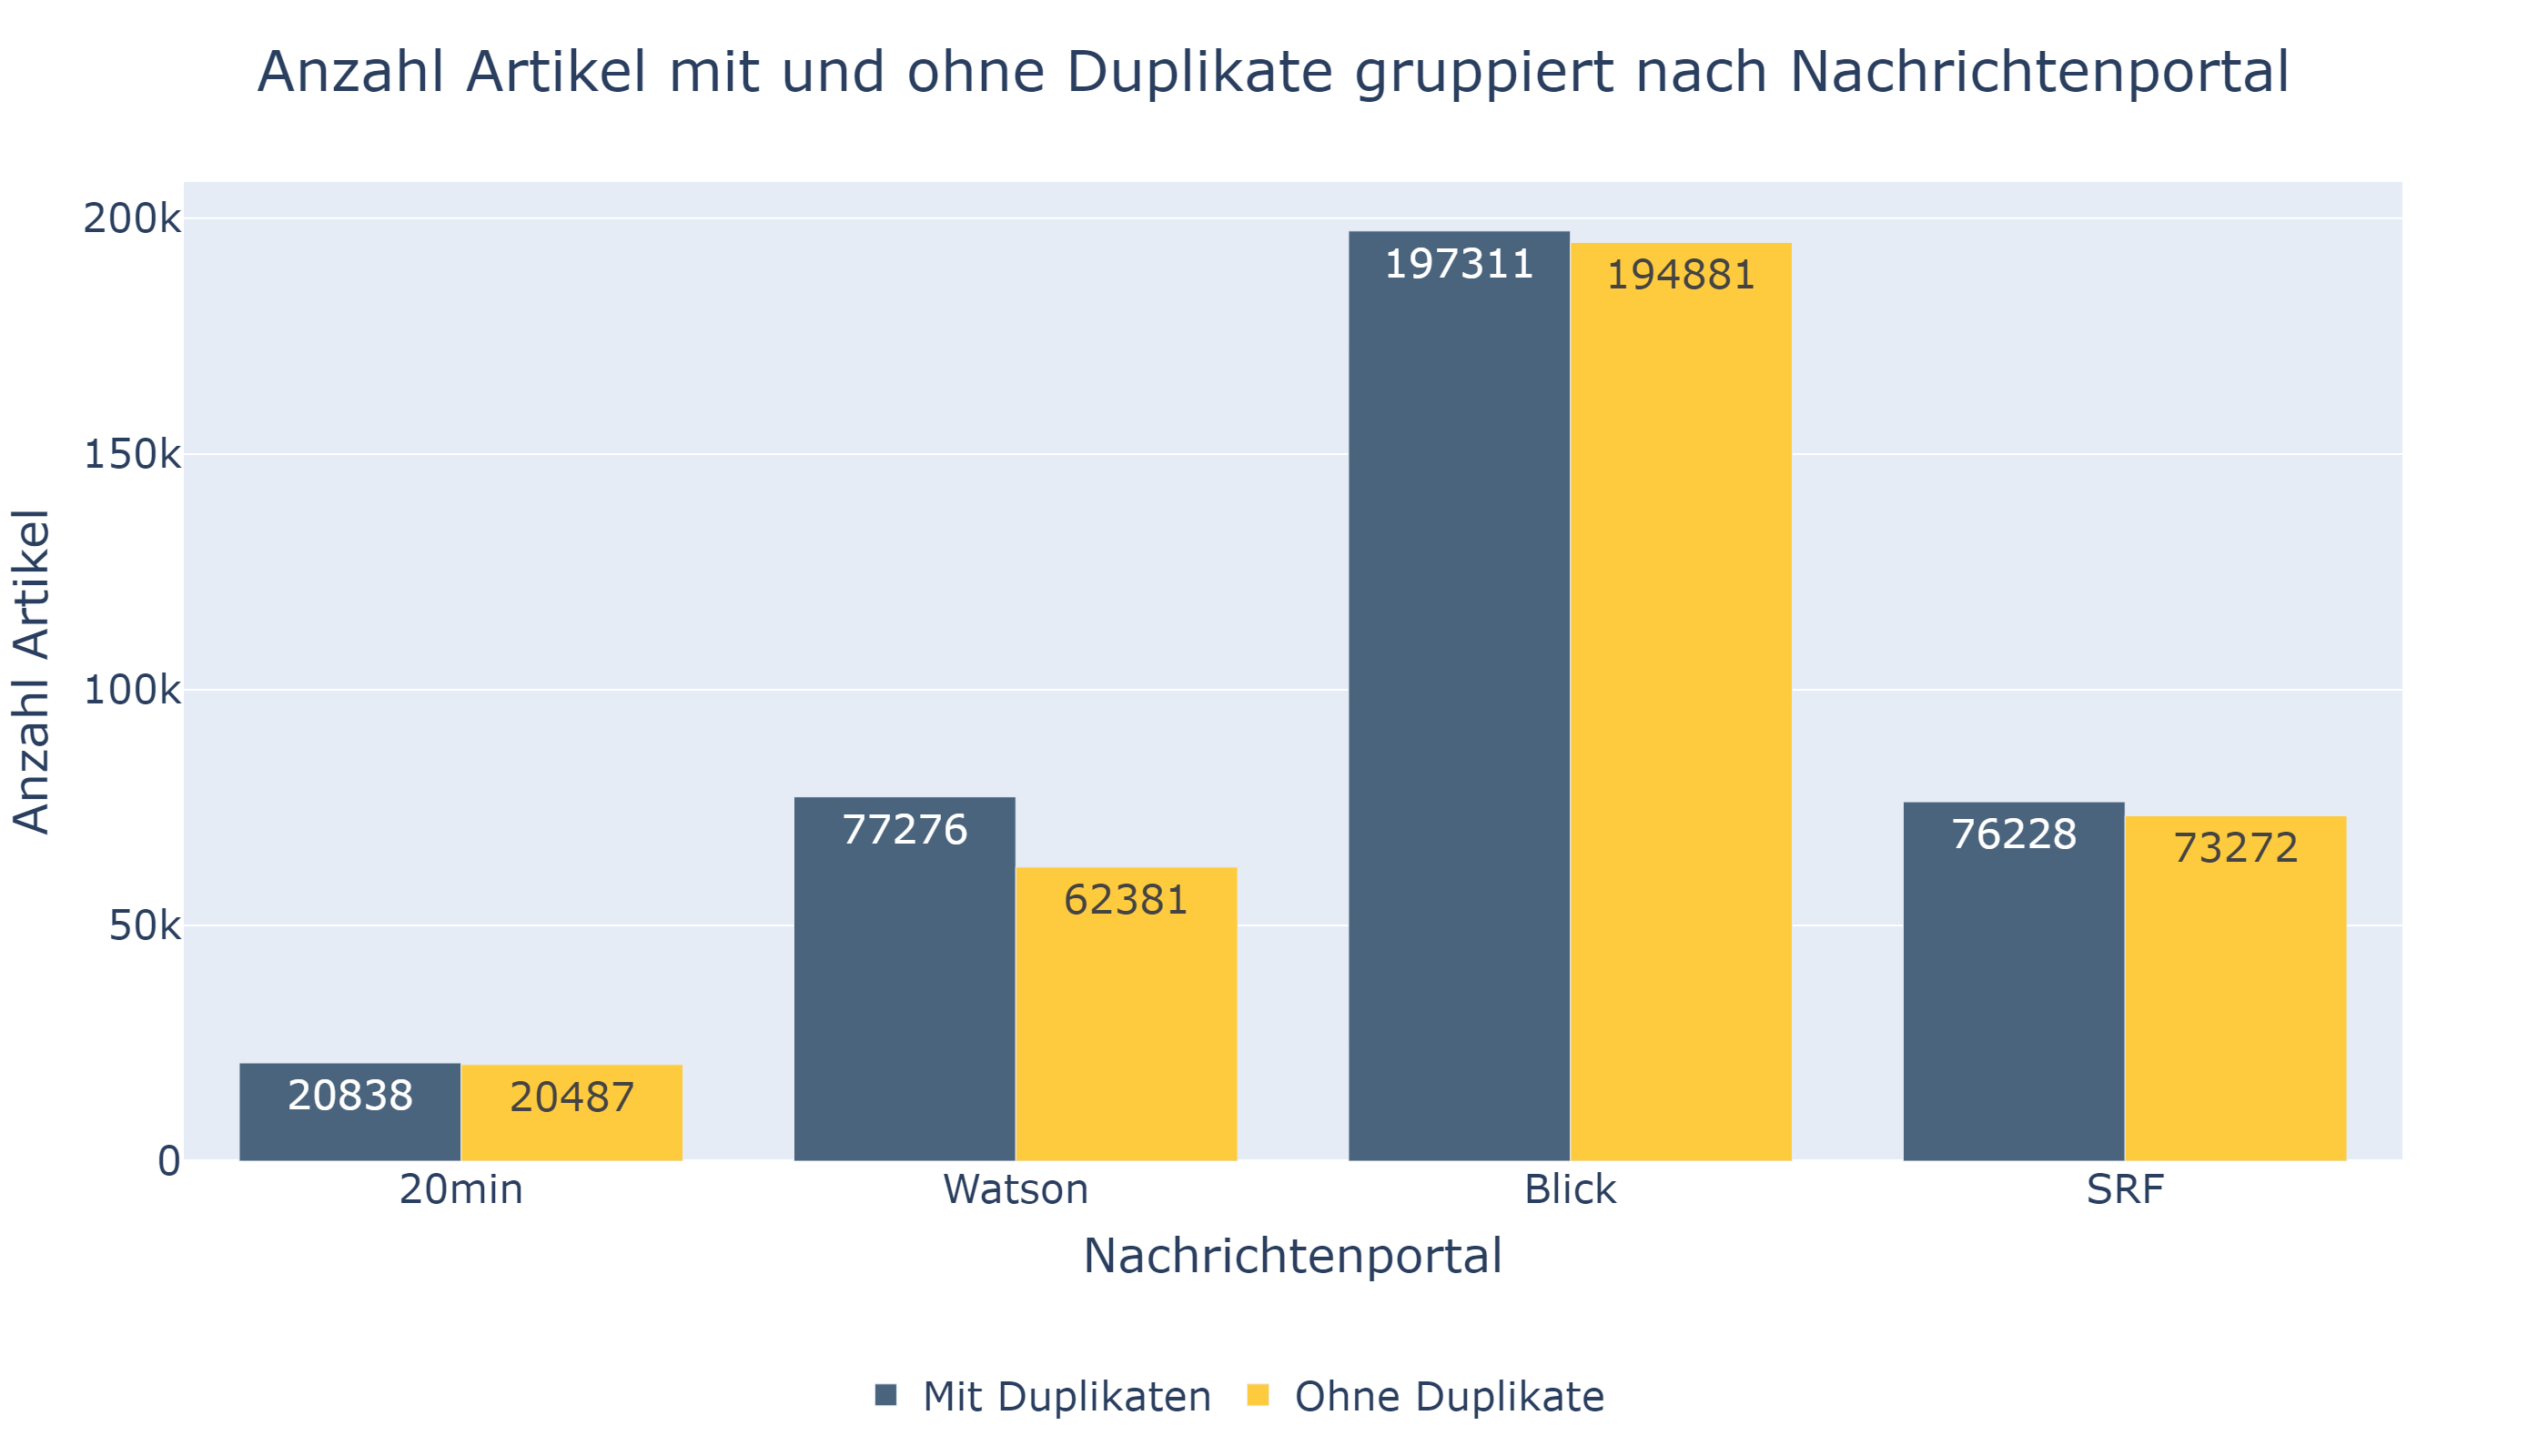
\includegraphics[width=1\linewidth]{./images/datenbereinigung.png}
		\caption{Anzahl Artikel vor und nach der Datenbereinigung}
		\label{datenbereinigung}
	\end{center}
\end{figure}

\section{Extraktion und Aggregation der Zitate}

Die folgenden zwei Abschnitte beschreiben die Verteilung der gefundenen Zitate pro
Nachrichtenportal und in einem weiteren Schritt zusätzlich pro Geschlecht. Der letztere Teil
beantwortet eigentliche Forschungsfrage zum \gl{gendergap}.

\subsection{Verteilung der Zitate pro Nachrichtenportal}

Das Ergebnis der in Kapitel \ref{citation-extraction} beschriebenen Extraktion der Zitate
resultierte in einer neuen MongoDB \gl{collection} \enquote{analyzed\_articles}. Diese enthält
für jeden Artikel der \gl{collection} \enquote{unique\_articles} die wichtigsten Artikelinformationen
plus die gefundenen Zitate. Insgesamt fanden wir 133'443 Zitate über alle
Nachrichtenportale. Die Grafik \ref{count-citations-per-portal} zeigt die Verteilung über die
Portale.

\begin{figure}[H]
	\begin{center}
        \centering
		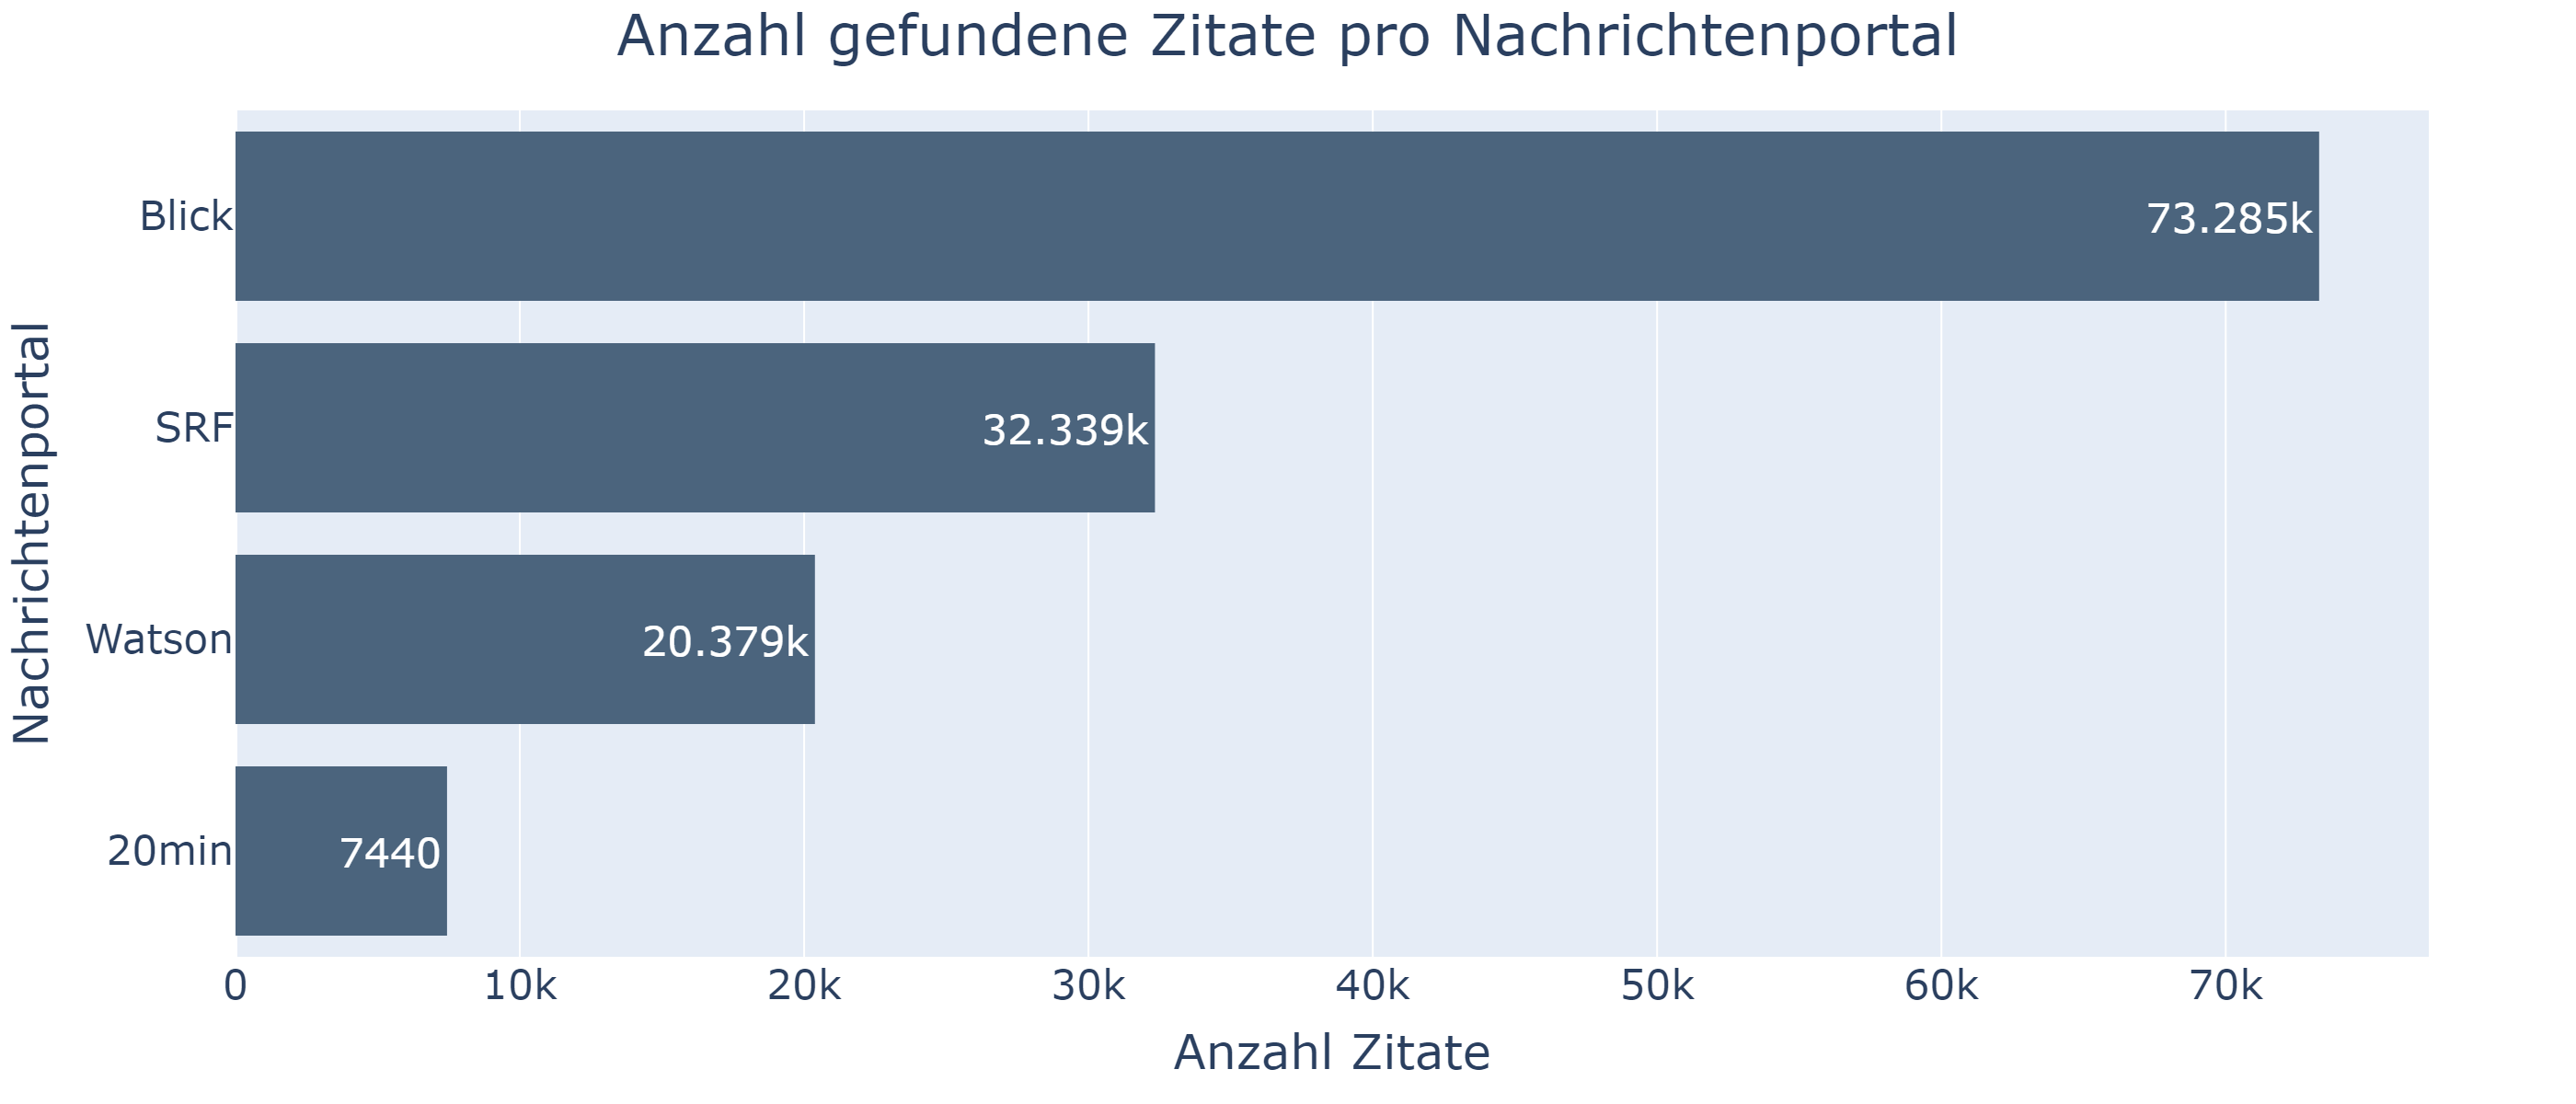
\includegraphics[width=1\linewidth]{./images/plot_anzahl_zitate_pro_portal.PNG}
		\caption{Anzahl gefundene Zitate}
		\label{count-citations-per-portal}
	\end{center}
\end{figure}

Der Algorithmus fand am meisten Zitate von Blick, gefolgt von SRF und Watson und am wenigsten
von 20min. Diese Verteilung ist nicht überraschend, wenn man die Verteilung der Anzahl Artikel bedenkt (vgl. Abbildung \ref{datenbereinigung}).

Eine spannende Erkenntnis ist im Diagramm in Abbildung \ref{citations-per-article} zu sehen,
das die Anzahl gefundener Zitate pro Portal pro Artikel darstellt. Mit einem Quotienten von
0.44 scheint SRF deutlich häufiger Zitate in seinen Artikeln zu verwenden als die anderen. Blick und 20min weisen
mit 0.38 resp. 0.36 einen ähnlichen Wert auf. Watson weist mit 0.33 Zitate den kleinsten Wert auf.

\begin{figure}[H]
	\begin{center}
        \centering
		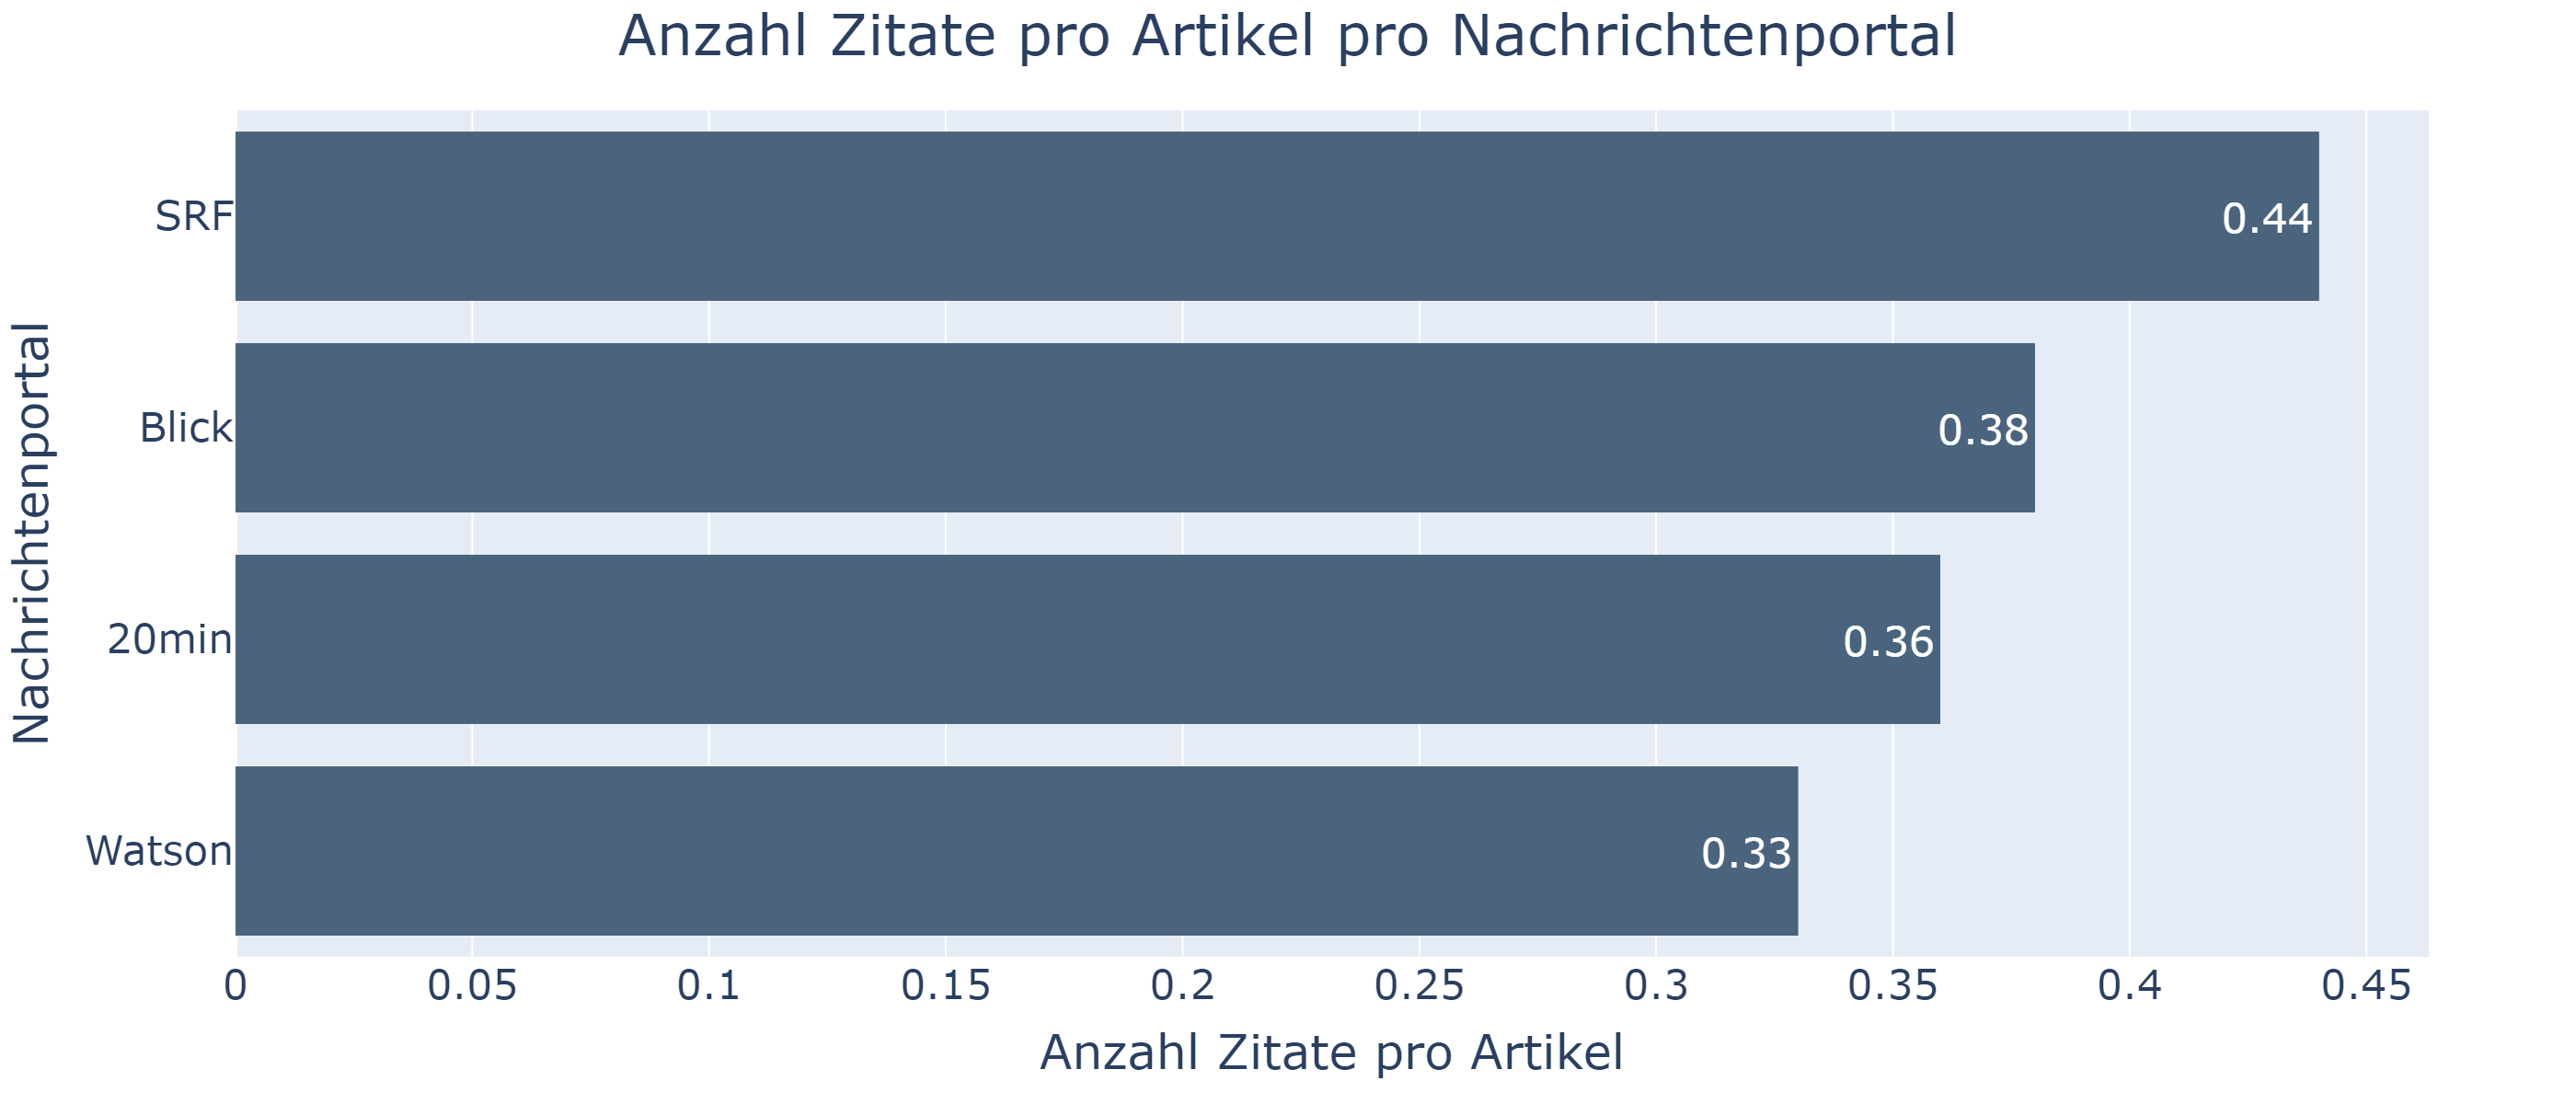
\includegraphics[width=1\linewidth]{./images/plot_zitate_pro_artikel.PNG}
		\caption{Anzahl gefundene Zitate pro Artikel pro Nachrichtenportal}
		\label{citations-per-article}
	\end{center}
\end{figure}



\subsection{Verteilung der Zitate pro Nachrichtenportal und pro Geschlecht}

Bevor wir in die Auswertung zum \gl{gendergap} in den Nachrichtenportalen eintauchen, möchten
wir nochmals betonen, dass die Zahlen ausschliesslich die auf unserem Datensatz gemessenen Resultate darstellen
und diese eine potenziell grosse Ungenauigkeit aufweisen (vgl. Kapitel \ref{quality-assurance}).

Gruppiert nach dem identifizierten Geschlecht ergibt sich eine Verteilung, die auf eine starke
Übervertretung von Zitaten von Männern hindeutet, wie die Abbildung \ref{sum-citations-stacked} zeigt.
So scheinen alle Nachrichtenportale eine ähnliche Verteilung aufzuweisen, in der gut zwei Drittel
der Zitate von Männern stammen und nur ein Fünftel oder ein Viertel von Frauen. Der Rest ist entsprechend
\enquote{unbekannt} zugeordnet. Diese Zuordnung bedeutet, dass der Algorithmus das Geschlecht der zitierten Person nicht ausfindig machen konnte.
Das arithmetische Mittel über die vier Portale liegt bei den Männern bei 65.6\% und bei den Frauen bei 21.2\%. Hinzu kommen 13.2\% der Kategorie \enquote{unbekannt}.
Diese Werte sind in der Abbildung \ref{sum-citations-stacked} zwischen den Portalen mit dem Label \enquote{Mittelwert} aufgelistet.
Aufgrund der limitierten Qualität (beschrieben im Kapitel \ref{quality-assurance})
können die kleinen Unterschiede nicht zum exakten Vergleich oder Ranking zwischen den Portalen verwendet werden.

\begin{figure}[H]
	\begin{center}
        \centering
		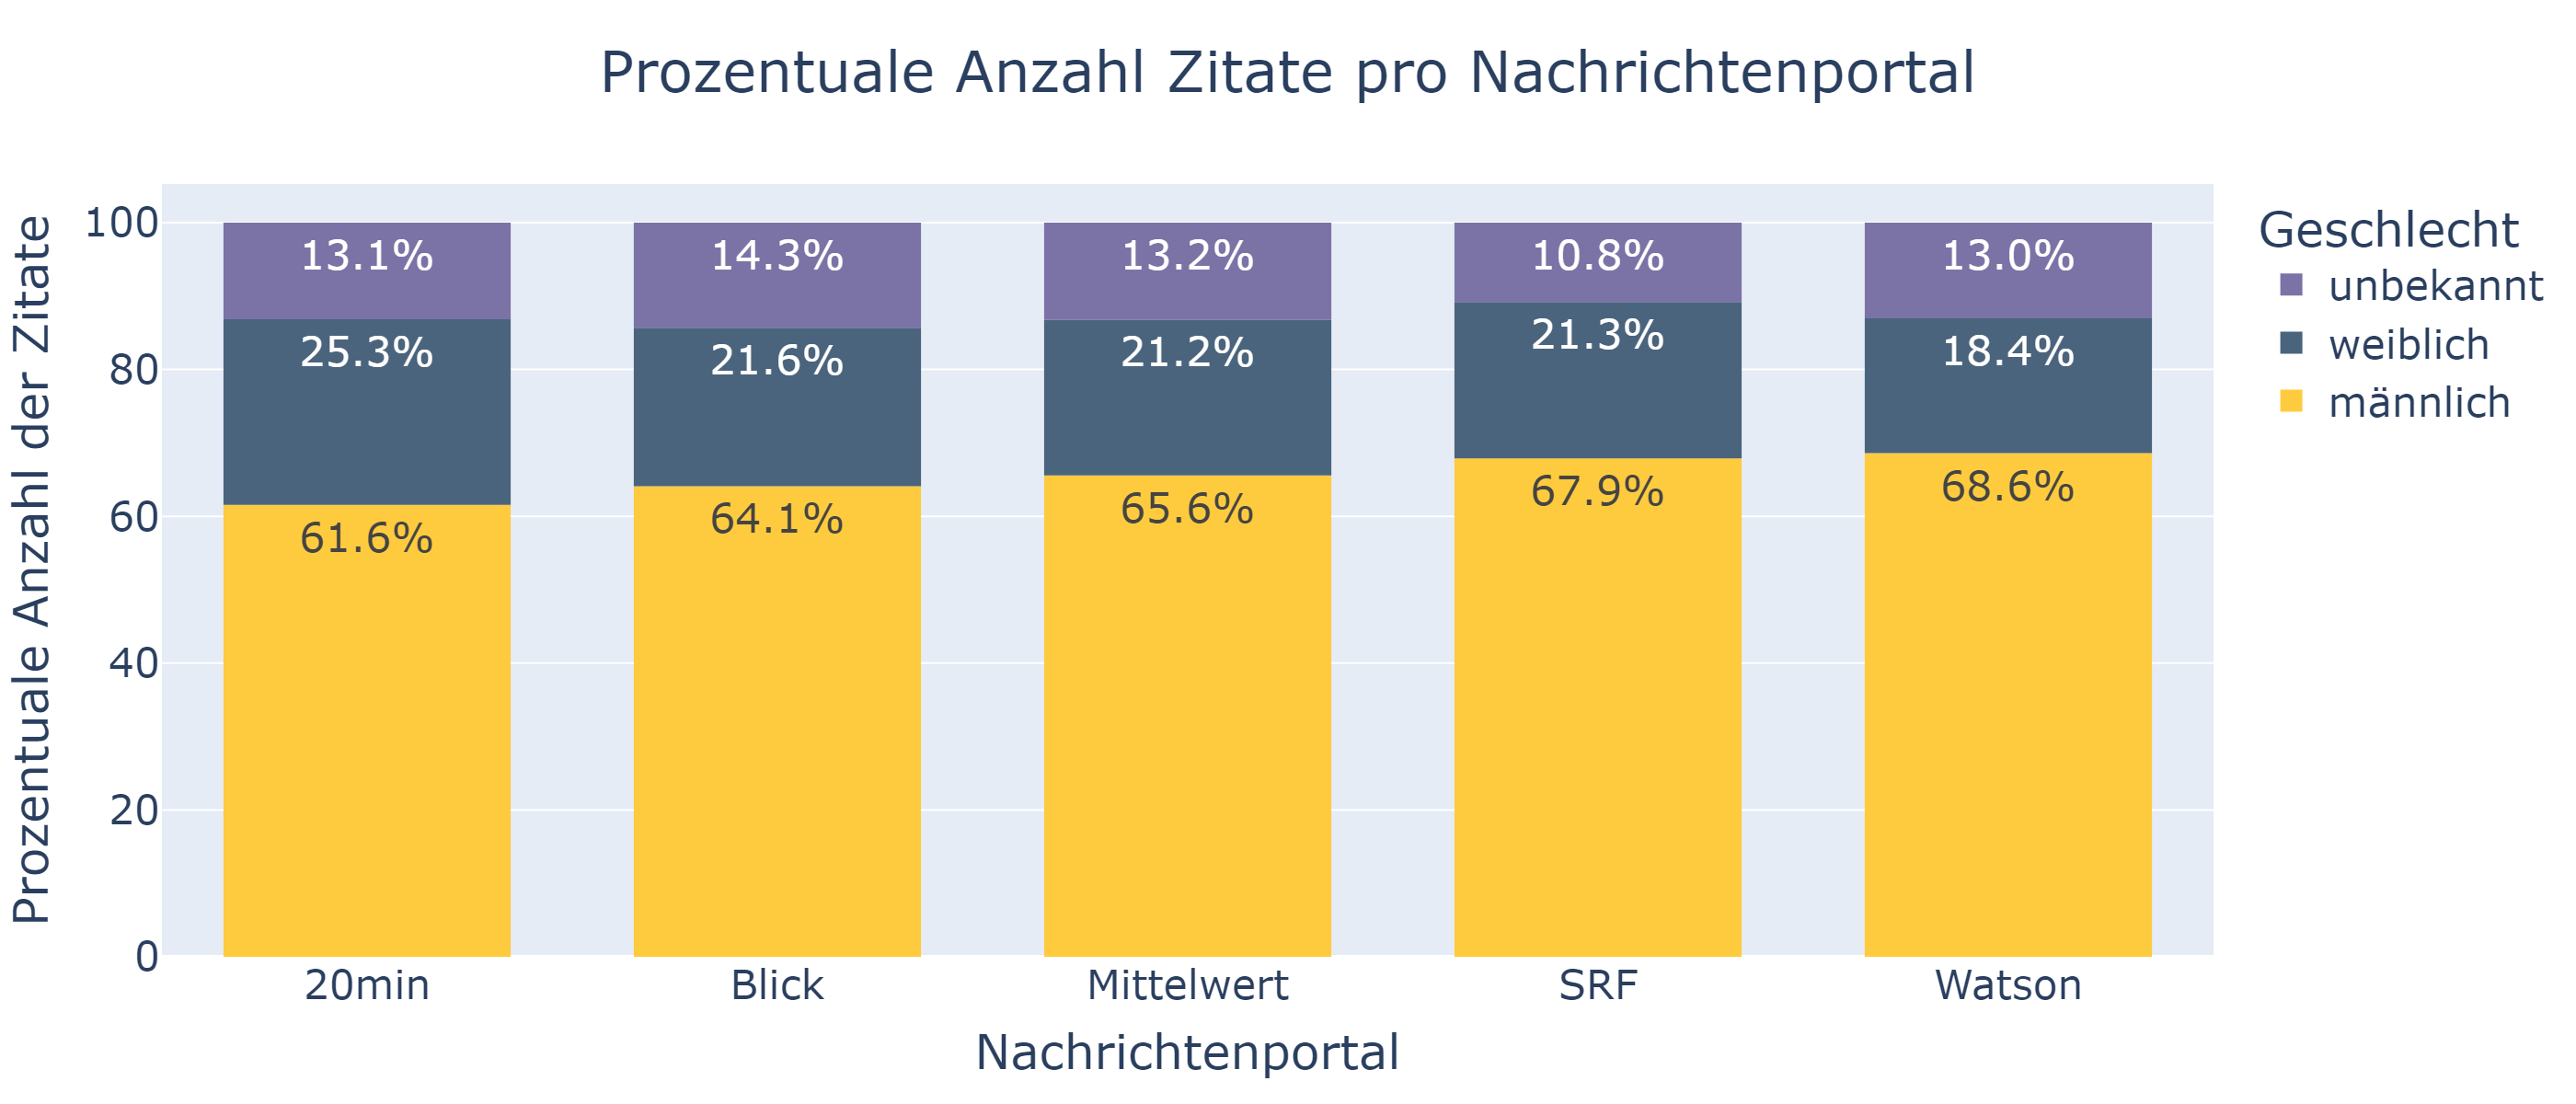
\includegraphics[width=1.1\linewidth]{./images/plot_zitate_pro_portal_geschlecht_stacked_prozentual.PNG}
		\caption{Prozentuale Anzahl Zitate pro Nachrichtenportal}
		\label{sum-citations-stacked}
	\end{center}
\end{figure}

Aufgrund dieser Resultate lässt sich nun endlich der \gl{gendergap} anhand der definierten Formel \ref{ggt-formula}
bestimmen. Dieser ist pro Portal in der Abbildung \ref{gender-gap-per-portal} dargestellt.

Sie zeigt, dass der Algorithmus bei Watson mit 57.7\% den grössten \gl{gendergap} messen konnte. SRF und Blick folgen mit 52.24\%
und 49.59\% respektive. Den kleinsten Gap fand er bei den Artikeln von 20min mit 41.77\%. Das arithmetische
Mittel über die Portale lag bei dieser Kennzahl bei 50.34\%, gekennzeichnet als \enquote{Mittelwert} in der Grafik.

Unter Berücksichtigung der Limitationen (vgl. Abschnitt \ref{limitations}) bedeutet diese Zahl, 
dass Frauen in unserem Datensatz im Schnitt 50.34\% weniger häufig zitiert werden als Männer.

\begin{figure}[H]
	\begin{center}
        \centering
		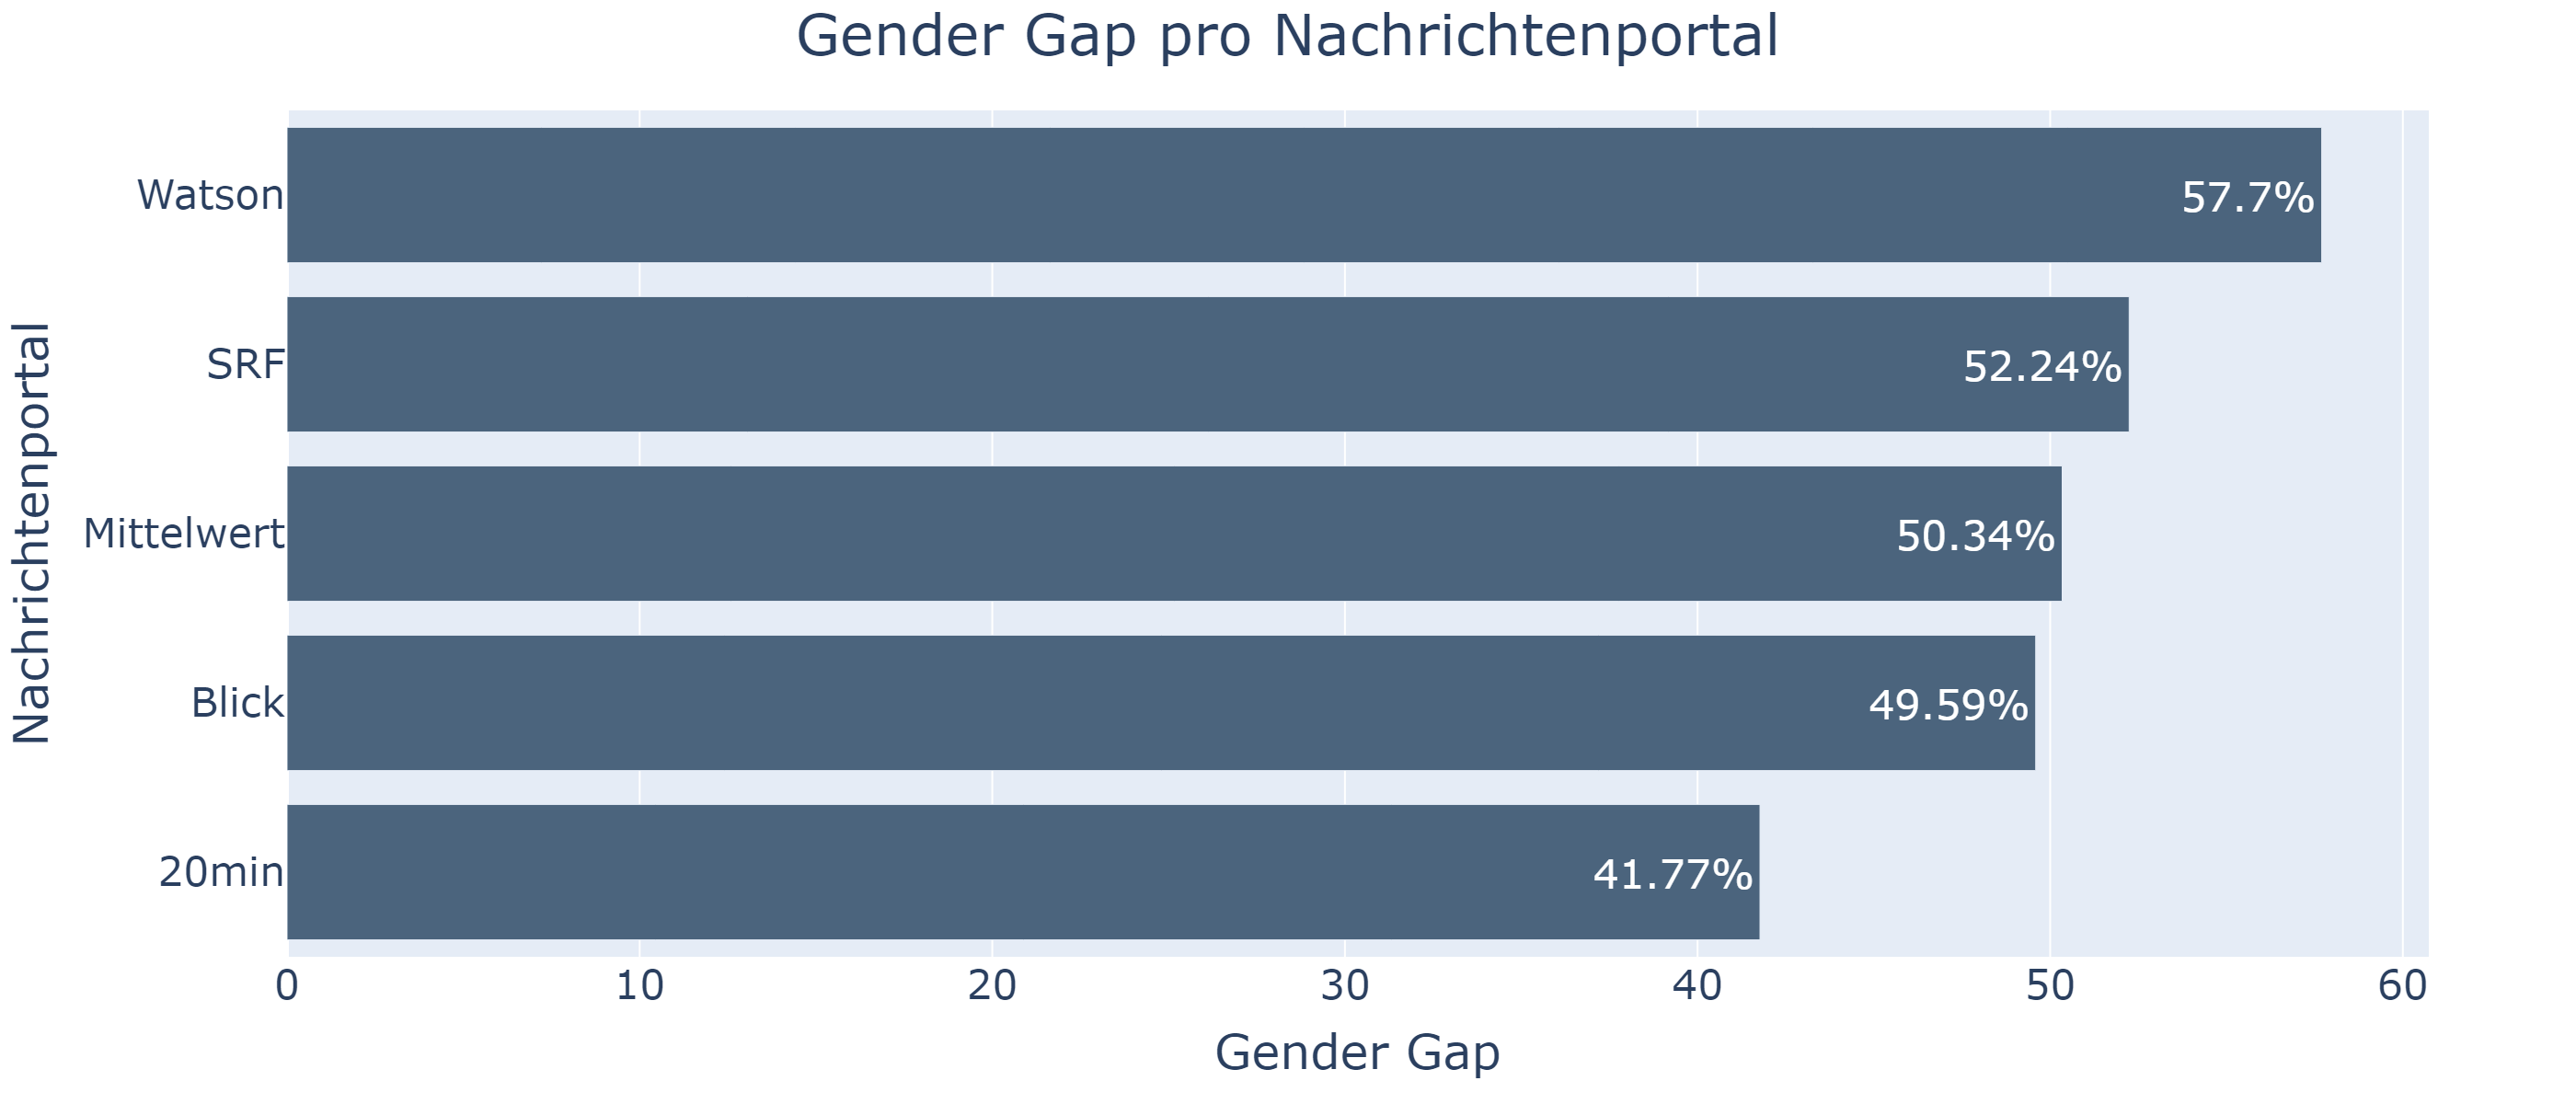
\includegraphics[width=1\linewidth]{./images/plot_gender_gap_pro_portal.PNG}
		\caption{Gender Gap pro Nachrichtenportal}
		\label{gender-gap-per-portal}
	\end{center}
\end{figure}

\section{Qualitätssicherung}\label{quality-assurance}

Die grossen Datenmengen in diesem Projekt verlangten einen methodischen Ansatz zum Validieren der Qualität,
da eine Überprüfung aller Resultate aufgrund der grossen Anzahl und der Zeiteinschränkung nicht machbar war.
Aufgrund des zeitlichen Rahmens war eine systematische Bewertung der Qualität der Ergebnisse
nur bei der Extraktion der Zitate machbar.
Um ein ganzheitlicheres Bild über die Qualität der Auswertung erhalten zu können,
müssten die anderen Teile auch systematisch getestet und bewertet werden.

Die Qualität der Funktionen zum Erkennen der Zitate und Bestimmen des Geschlechts wurden ebenfalls mithilfe von
Gradings sichergestellt. Diese waren besonders während dem Entwickeln relevant und wurden deshalb aus praktischen Gründen
nicht weiter verfeinert. Die Algorithmen funktionieren mit zufriedenstellender Qualität, gemessen an Stichproben,
die wir von Hand durchgeführt haben.

Weil die Extraktion der Zitate im Gegensatz dazu keiner eindeutigen Logik folgen kann, war es für die Entwicklung dieses Algorithmus
wichtig, die Qualität und die Verbesserung des Algorithmus zu messen. Dies ermöglicht es uns ausserdem die Qualität
der Resultate abzuschätzen. 
Ein eigens dafür entwickelter Bewertungsalgorithmus soll einen möglichst guten Überblick über die Anzahl
der gefundenen Zitate und deren Qualität geben.

Dazu haben wir in manueller Arbeit pro Nachrichtenportal fünf Artikel ausgewertet und als JSON abgelegt. Insgesamt ergeben
sich daraus 20 Test-Artikel. Der Bewertungsalgorithmus ruft die Funktionalität zum Extrahieren der Zitate mit dem rohen
Text der Artikel auf und vergleicht das Resultat im Anschluss mit den manuell erstellten Lösungen. Als wichtigste Metrik
dient dabei der \enquote{Recall} (Abbildung \ref{recall-formula}).

\subsection{Recall}

Diese Metrik wird häufig auch im \gl{ml} verwendet, um die Genauigkeit des trainierten
Modells zu messen. Der Recall sagt in unserem Fall aus, wie viele der relevanten Zitate der Algorithmus finden konnte.
Der Recall ist die Prozentzahl der totalen Anzahl Zitate, die er hätte finden können.

\begin{figure}[H]
    \begin{equation}
        Recall = \frac{Anzahl \, gefundene \, Zitate}{Totale \, Anzahl \, Zitate}
    \end{equation}
    \caption{Formel Recall}
    \label{recall-formula}
\end{figure}

Als gefundene Zitate zählt der Bewertungsalgorithmus all diejenigen Zitate, die eine Qualität von
mindestens 60\% aufweisen. Mehr dazu in Kapitel \ref{quality-grade}
Die nachfolgende Abbildung \ref{piechart-recall} visualisiert den Recall von 61.2\% über
alle Nachrichtenportale.
Dieser Wert sagt aus, dass das Programm von allen vorhandenen Zitaten in den Lösungen
61.2\% gefunden hat.

\begin{figure}[H]
	\begin{center}
        \centering
		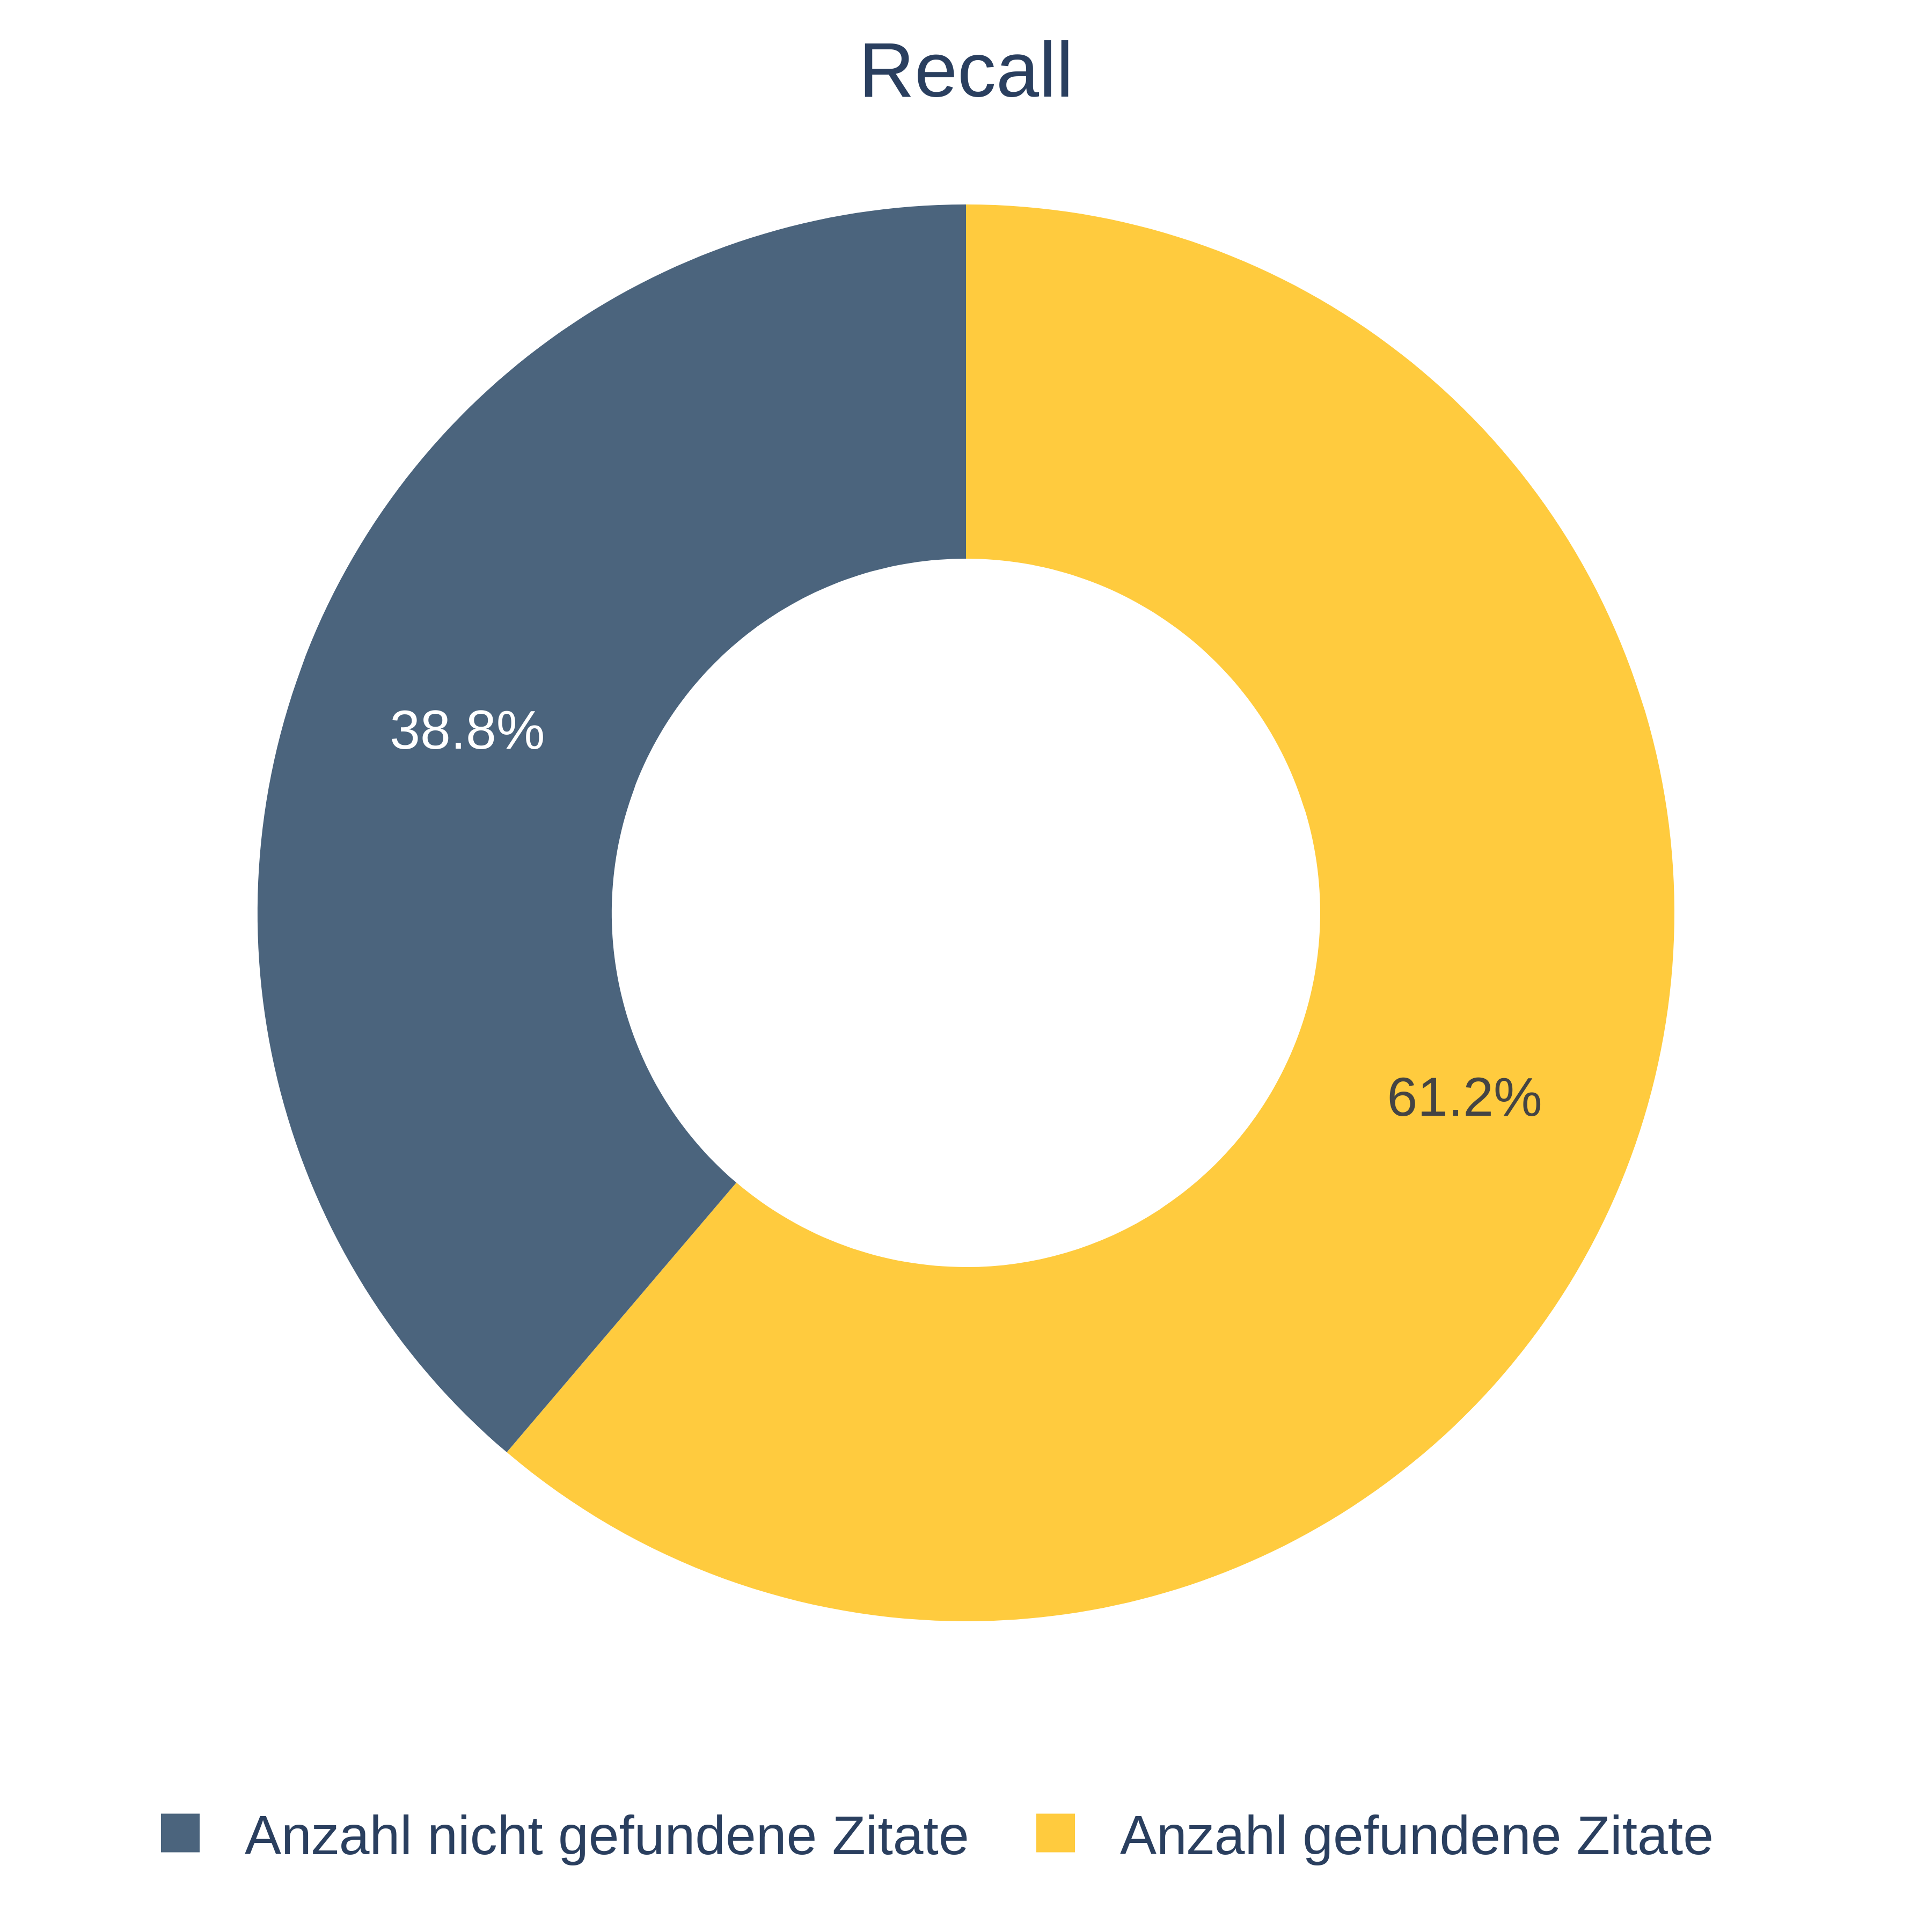
\includegraphics[width=0.75\linewidth]{./images/recall.png}
	\end{center}
	\caption{Recall der Zitate auf dem Testset}
	\label{piechart-recall}
\end{figure}

Das untenstehende Balkendiagramm \ref{barchart-recall} bietet einen Überblick
über die Performance aufgeschlüsselt nach Nachrichtenportal. Es fällt auf, dass
die Daten von Blick mit 70.6\% deutlich besser analysiert werden konnten als diejenigen
von 20min mit 50.0\%.

Wahrscheinlich ist diese Diskrepanz auf die geringe Anzahl Testfälle zurückzuführen.
Mit mehr Testfällen würde sich der Wert wahrscheinlich bei allen Nachrichtenportalen bei
60\% einpendeln.

\begin{figure}[H]
	\begin{center}
        \centering
		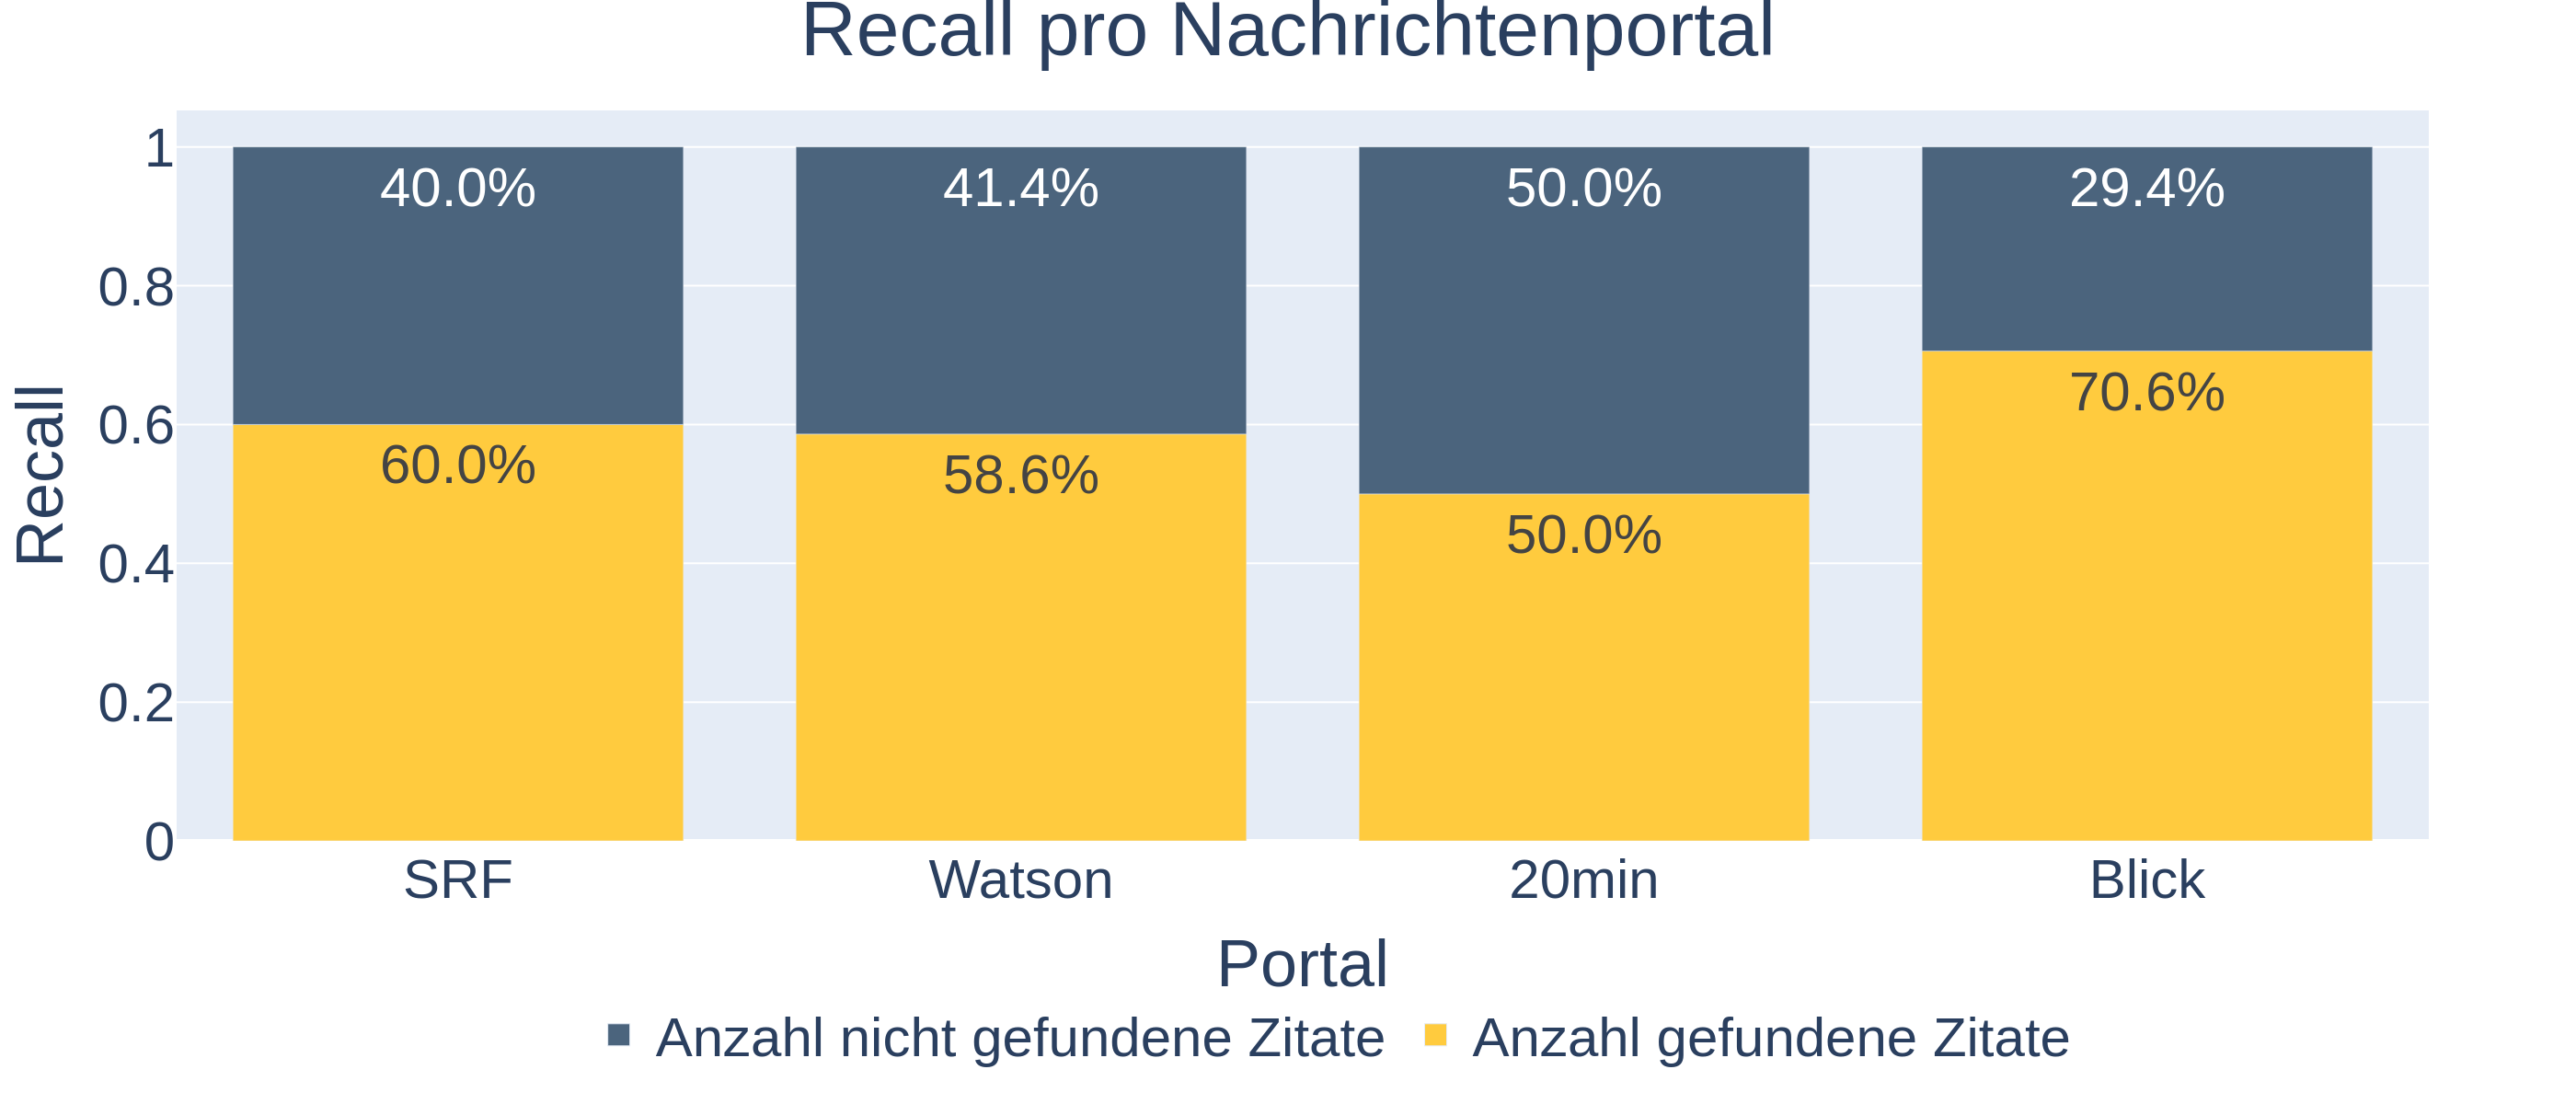
\includegraphics[width=1.0\linewidth]{./images/recall_portals.png}
	\end{center}
	\caption{Recall der Zitate pro Nachrichtenportal}
	\label{barchart-recall}
\end{figure}

\subsection{Qualitätsnote}\label{quality-grade}

Die Qualitätsnote setzt sich aus dem Durchschnitt der Stringähnlichkeiten der extrahierten Zitate
mit der Lösung zusammen. Zum Bestimmen der Stringähnlichkeit verwendet der Algorithmus den
\enquote{SequenceMatcher}\footnote{https://docs.python.org/3/library/difflib.html\#difflib.SequenceMatcher} von Python.
Dieser findet den länsten übereinstimmenden Substring aus zwei Strings relativ zur
Länge der beiden zu vergleichenden Strings.

Die Vermutung, dass die geringe Anzahl Tests Schwankungen in der Qualität verursacht
wird durch den Überblick in den folgenden Diagrammen (vgl. Abbildung \ref{histogram-grades}) gestützt.
20min hat deutlich weniger Zitate in den Lösungen als die anderen Nachrichtenportale.

Die Histogramme legen ausserdem nahe, dass die Rate der False-Positives gering ist.
Denn diese machen sich durch eine tiefe Note bemerkbar, da sie sehr unähnlich zu den Zitaten
aus den Lösungen sind. Dass davon wenige zu erkennen sind, suggeriert, dass False Positives
selten sind.

\begin{figure}[H]
	\begin{tabular}{ll}
		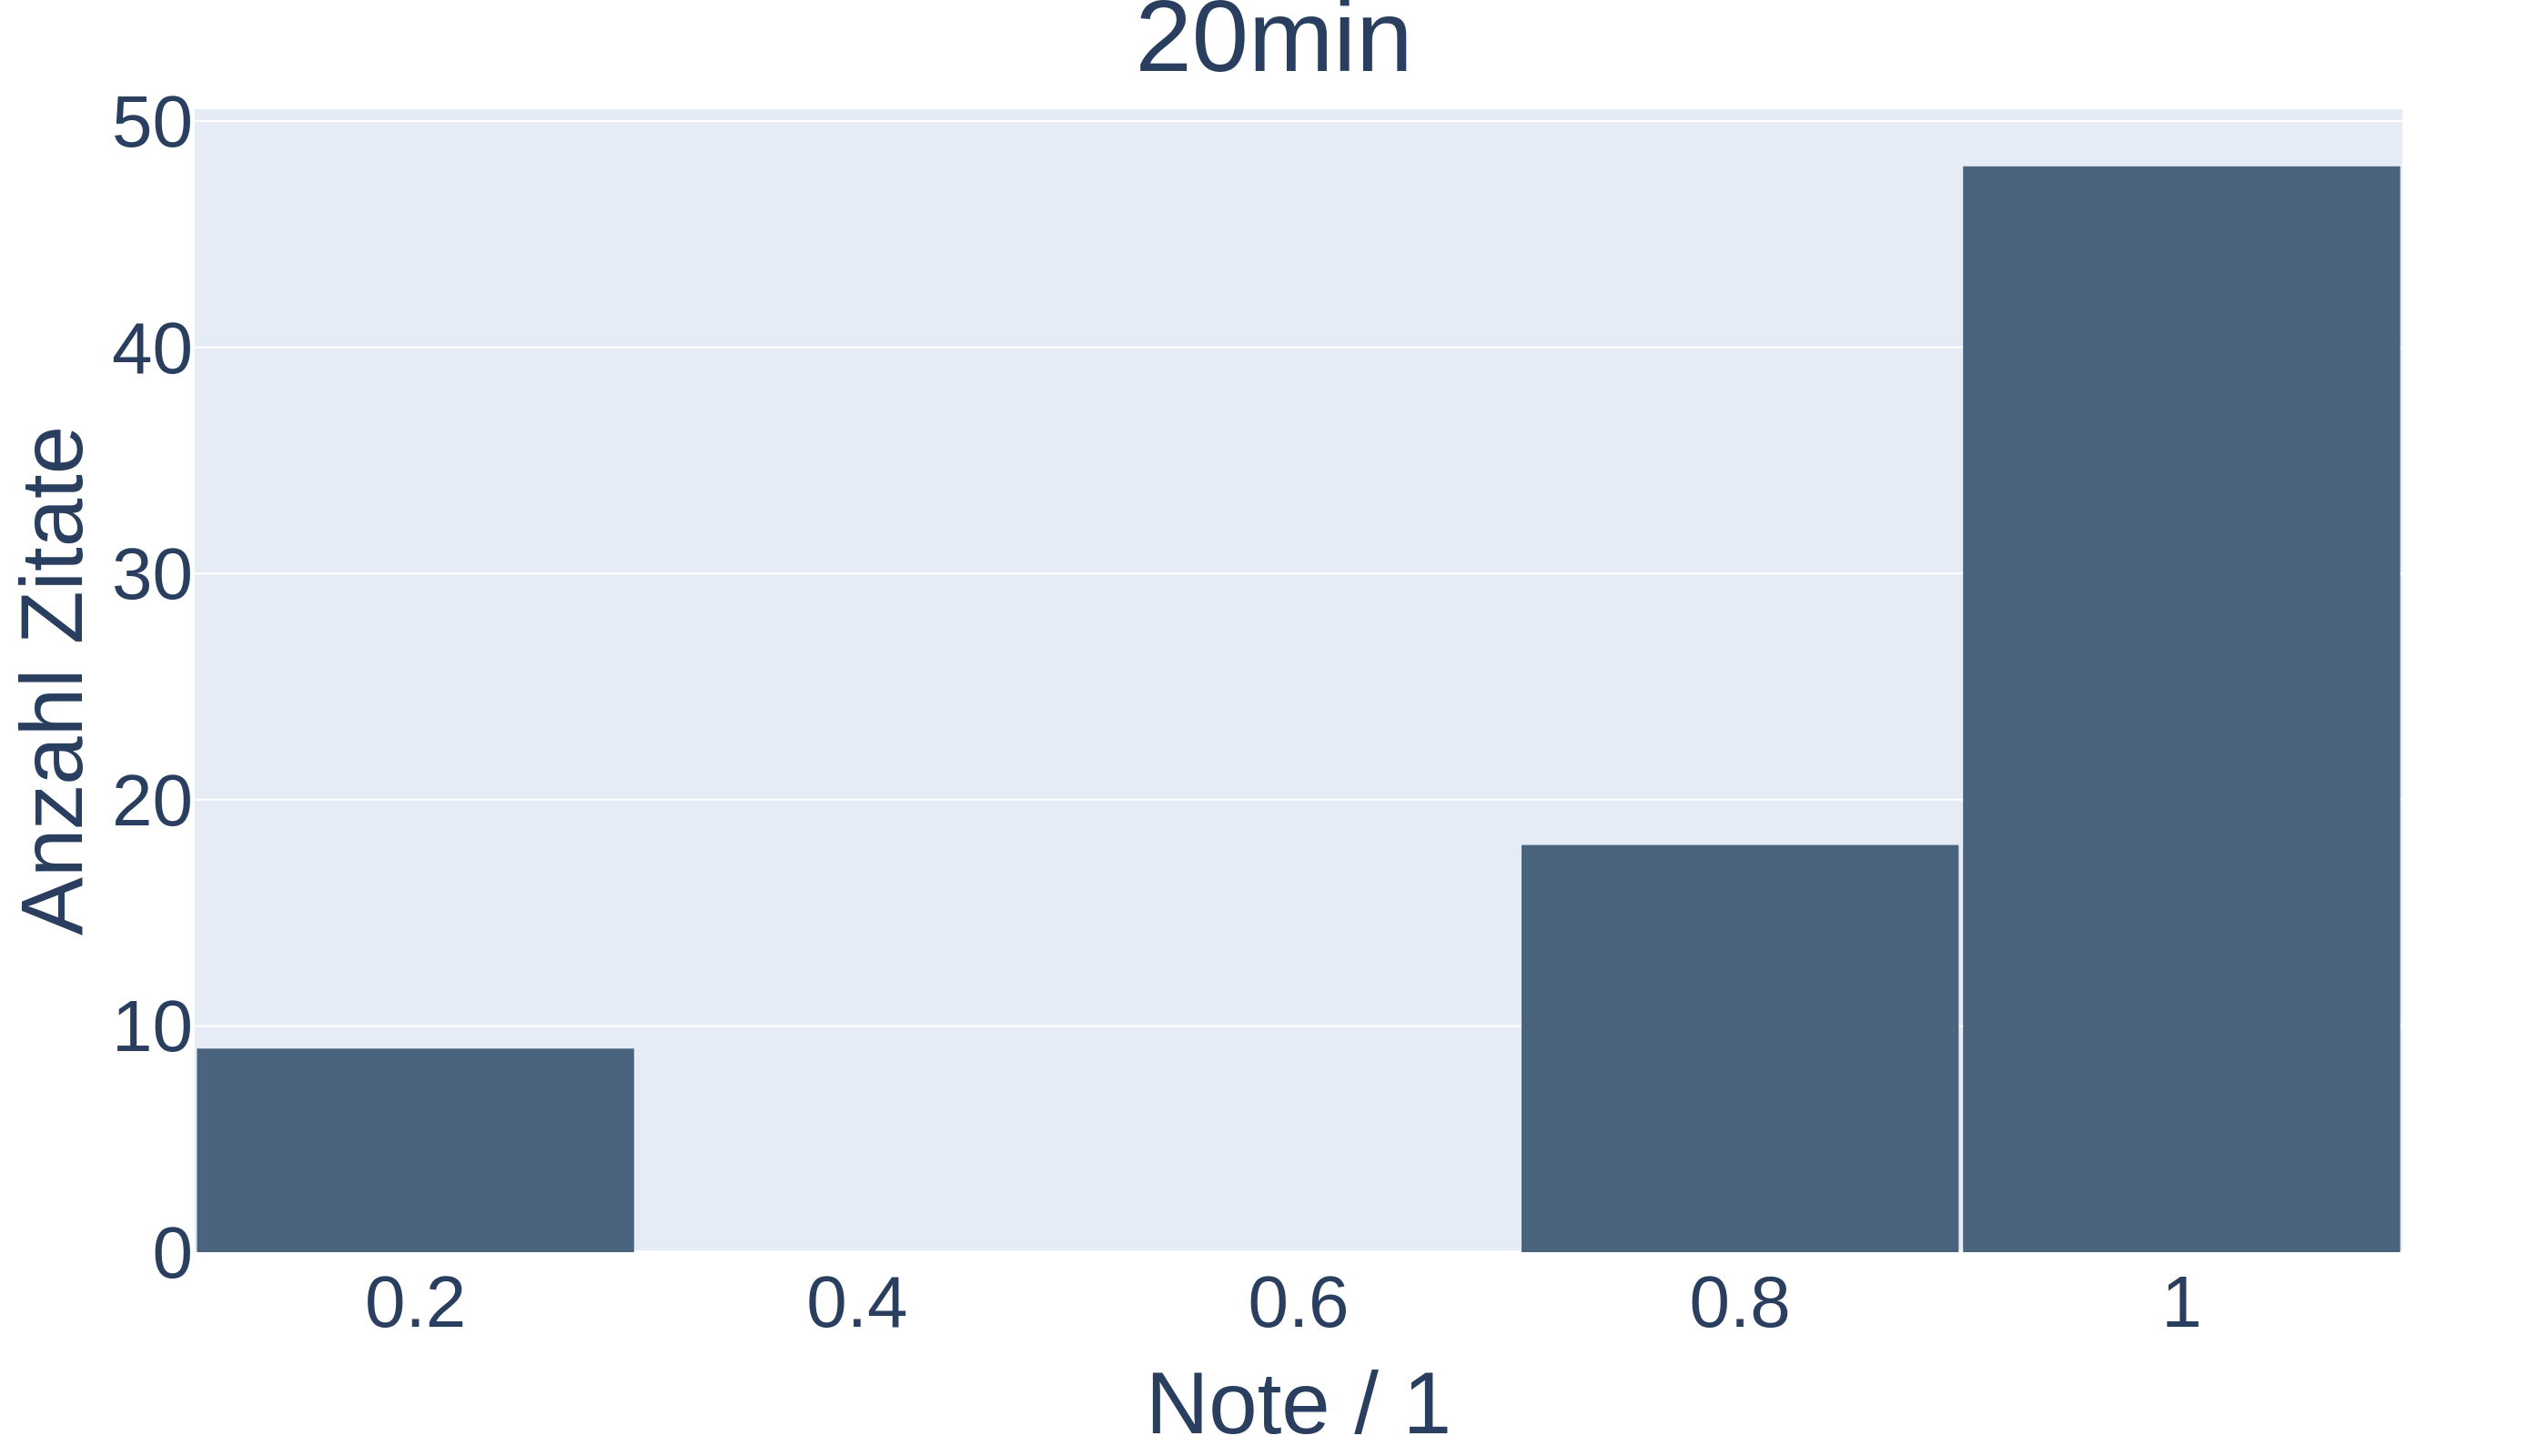
\includegraphics[width=.5\linewidth]{./images/citation_grades_20min.png} & 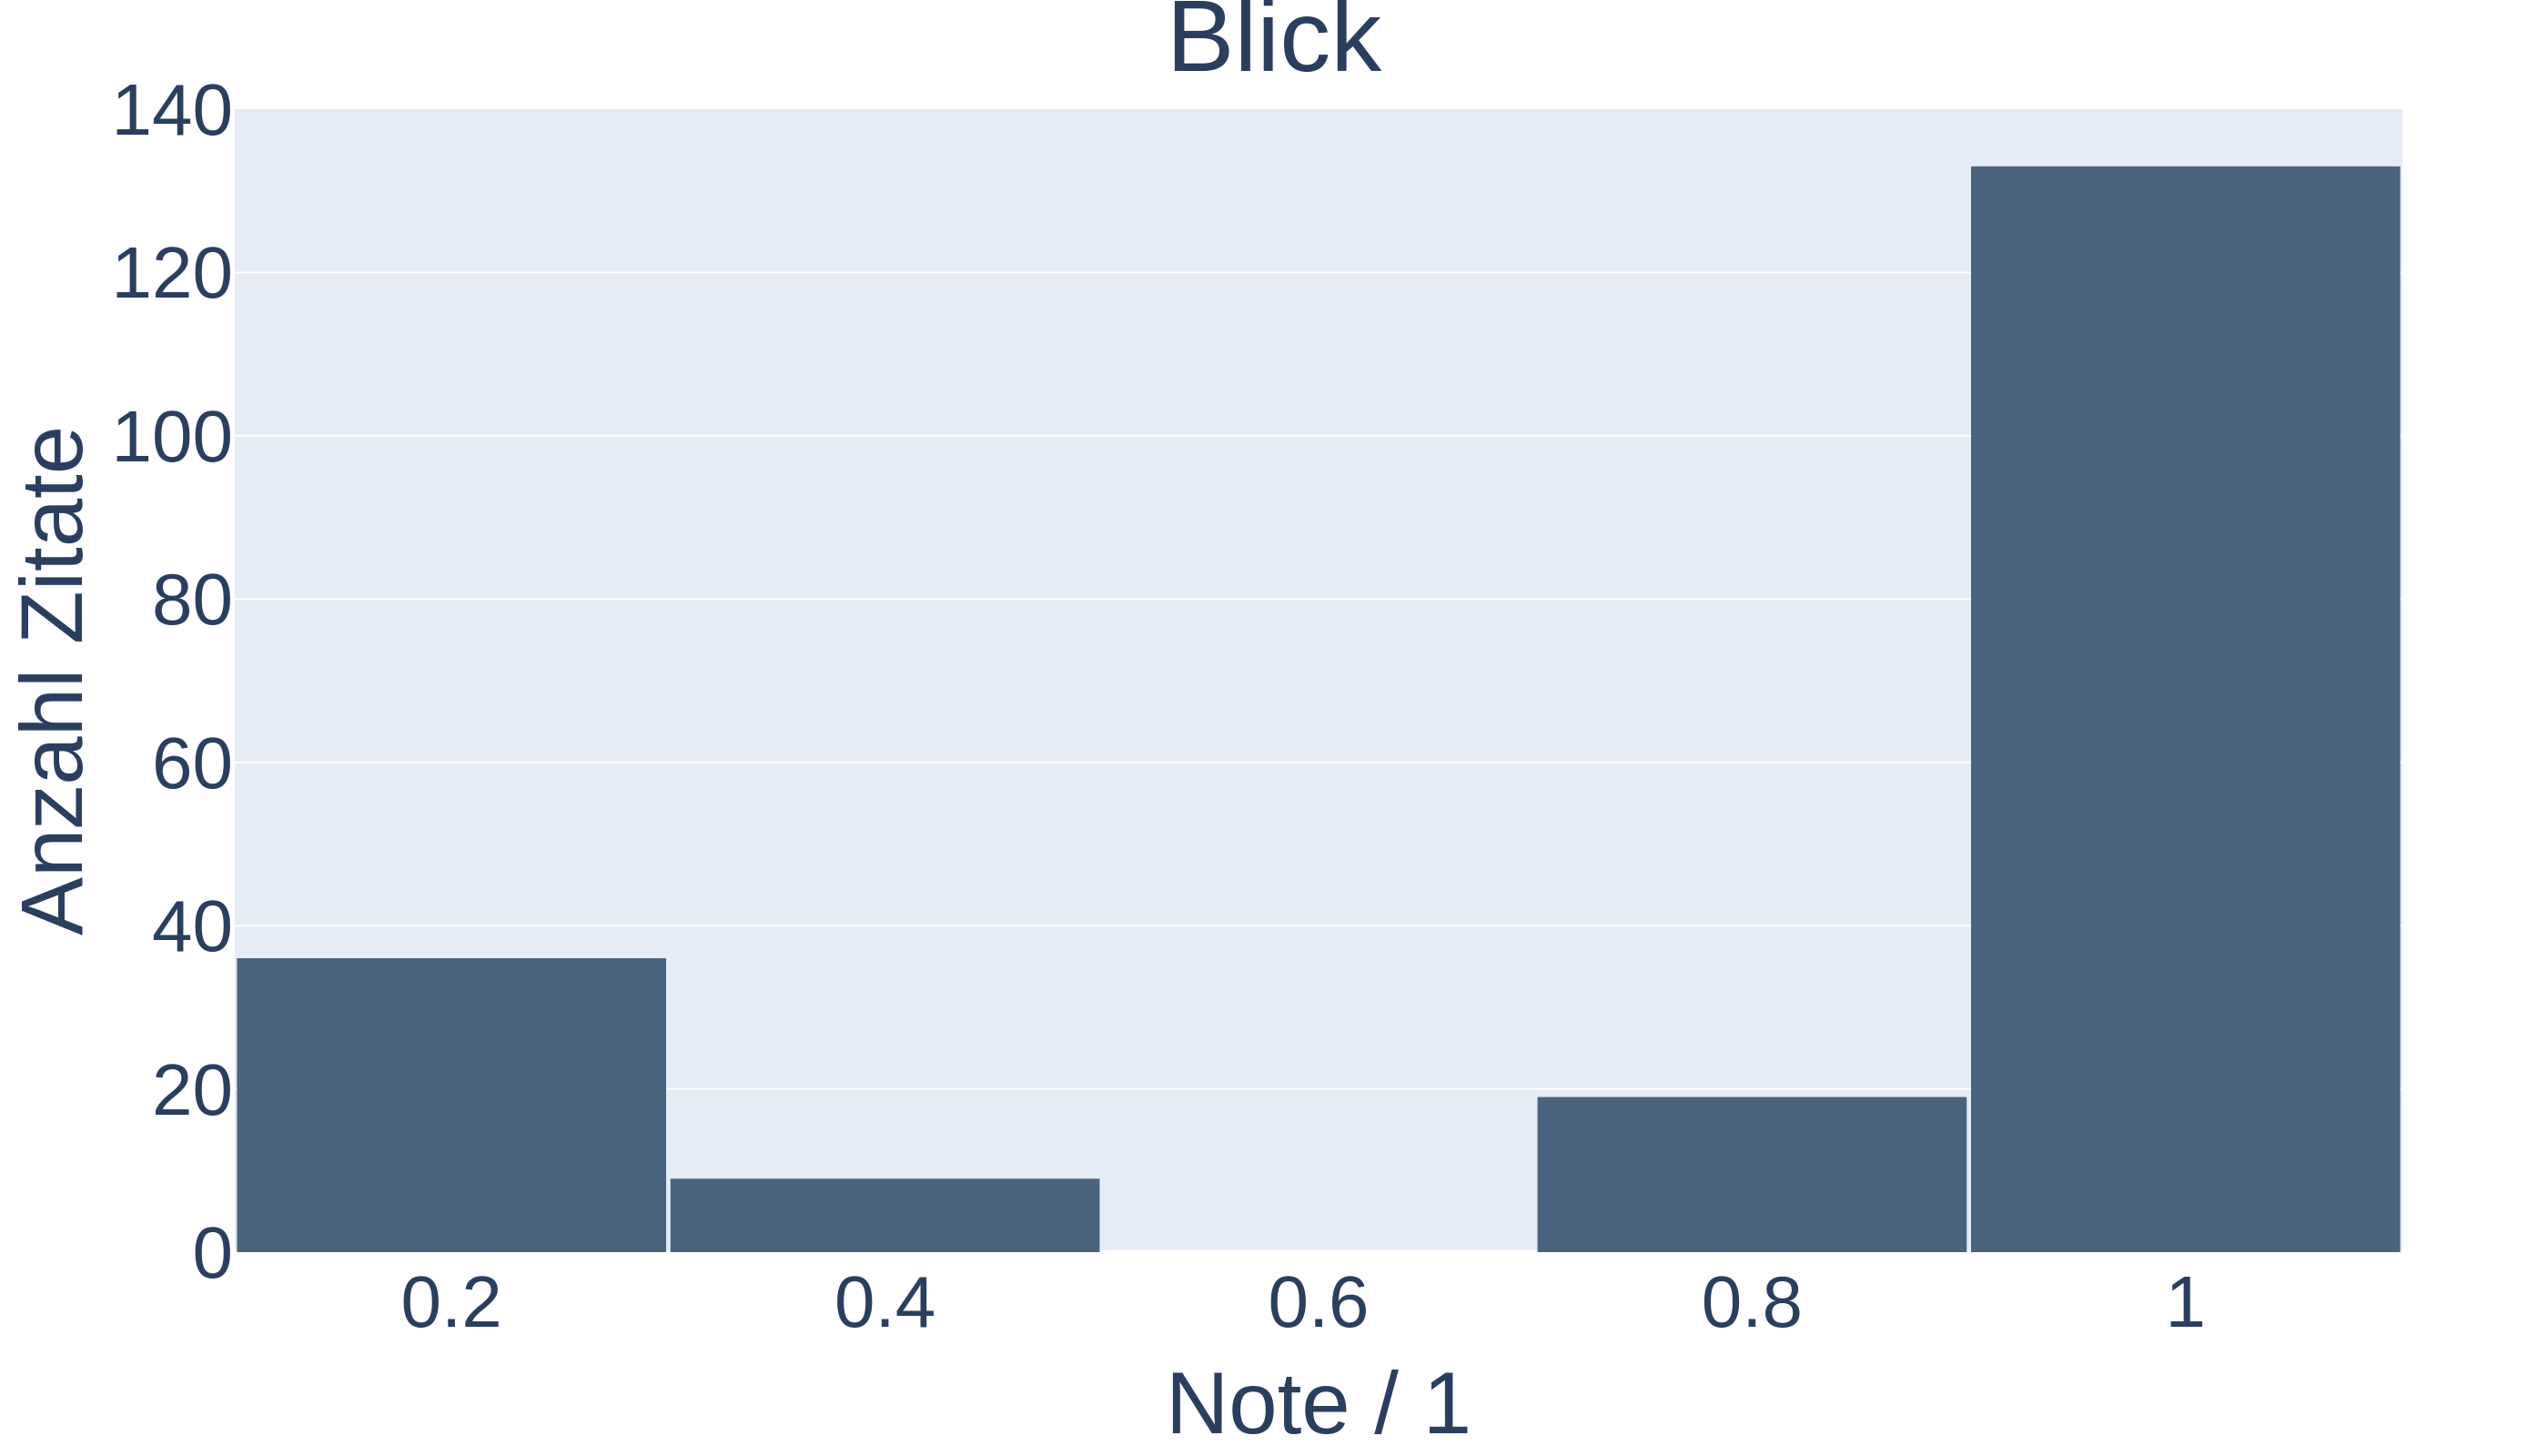
\includegraphics[width=.5\linewidth]{./images/citation_grades_blick.png} \\
		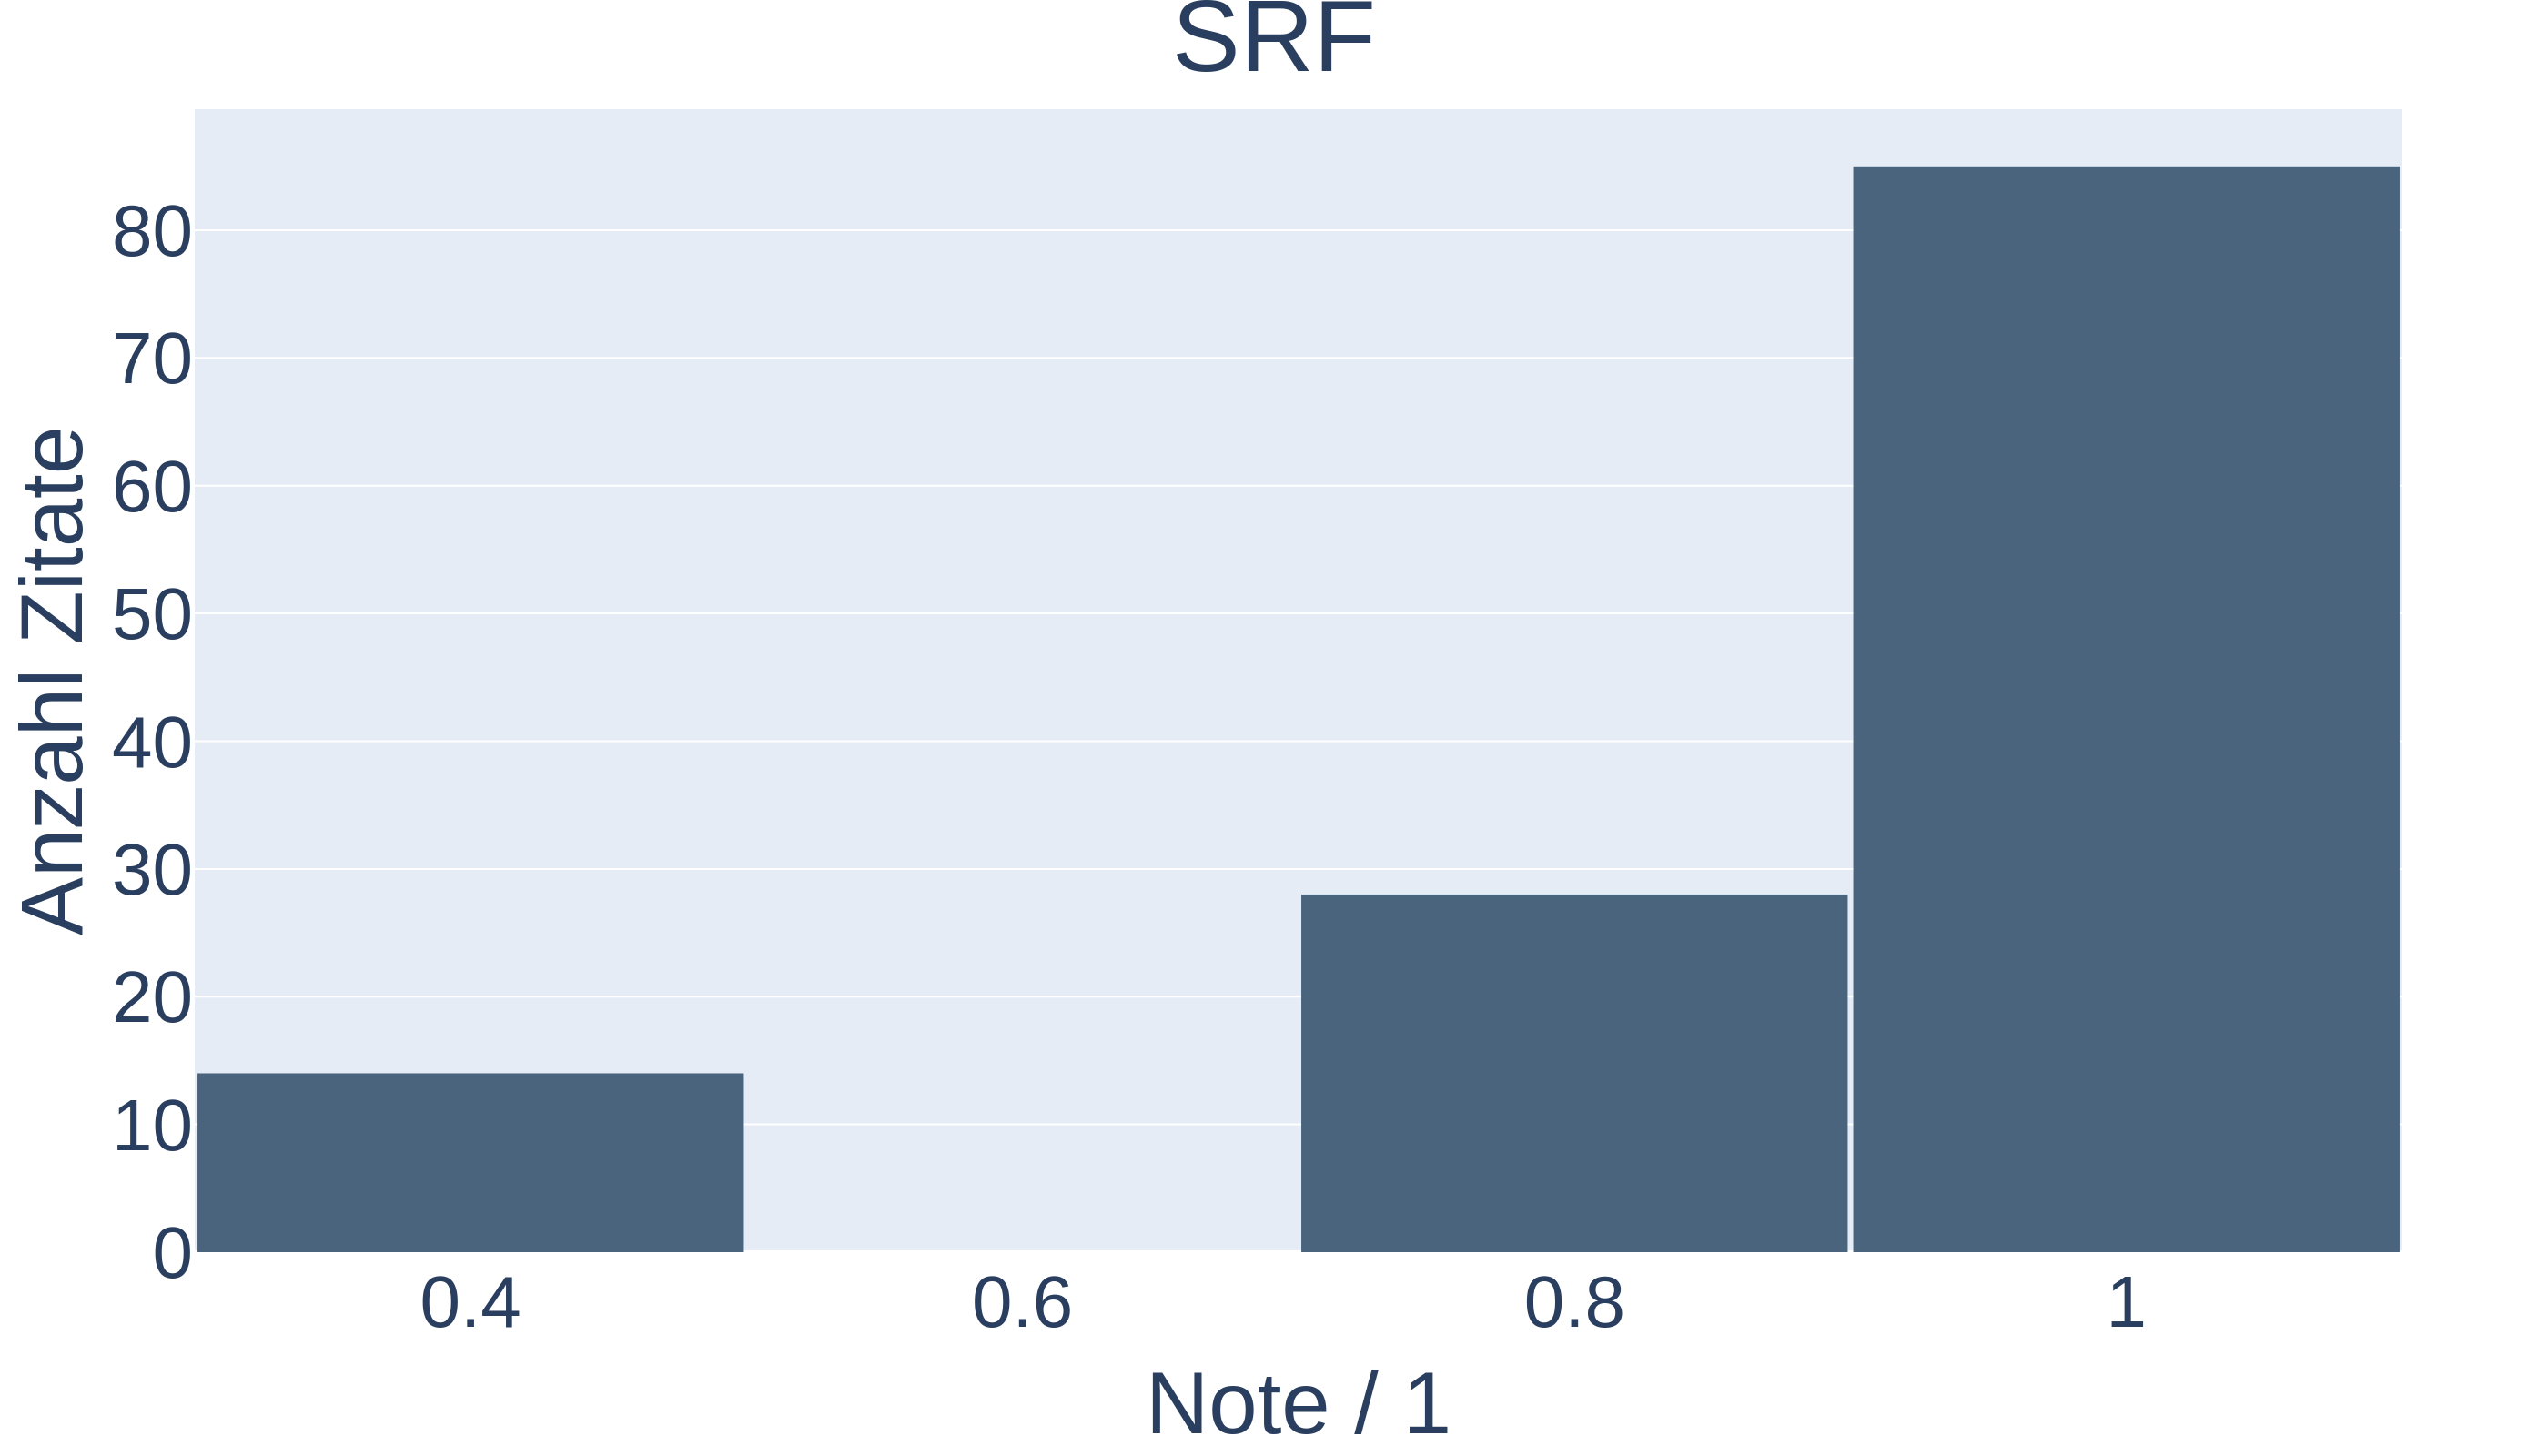
\includegraphics[width=.5\linewidth]{./images/citation_grades_srf.png} & 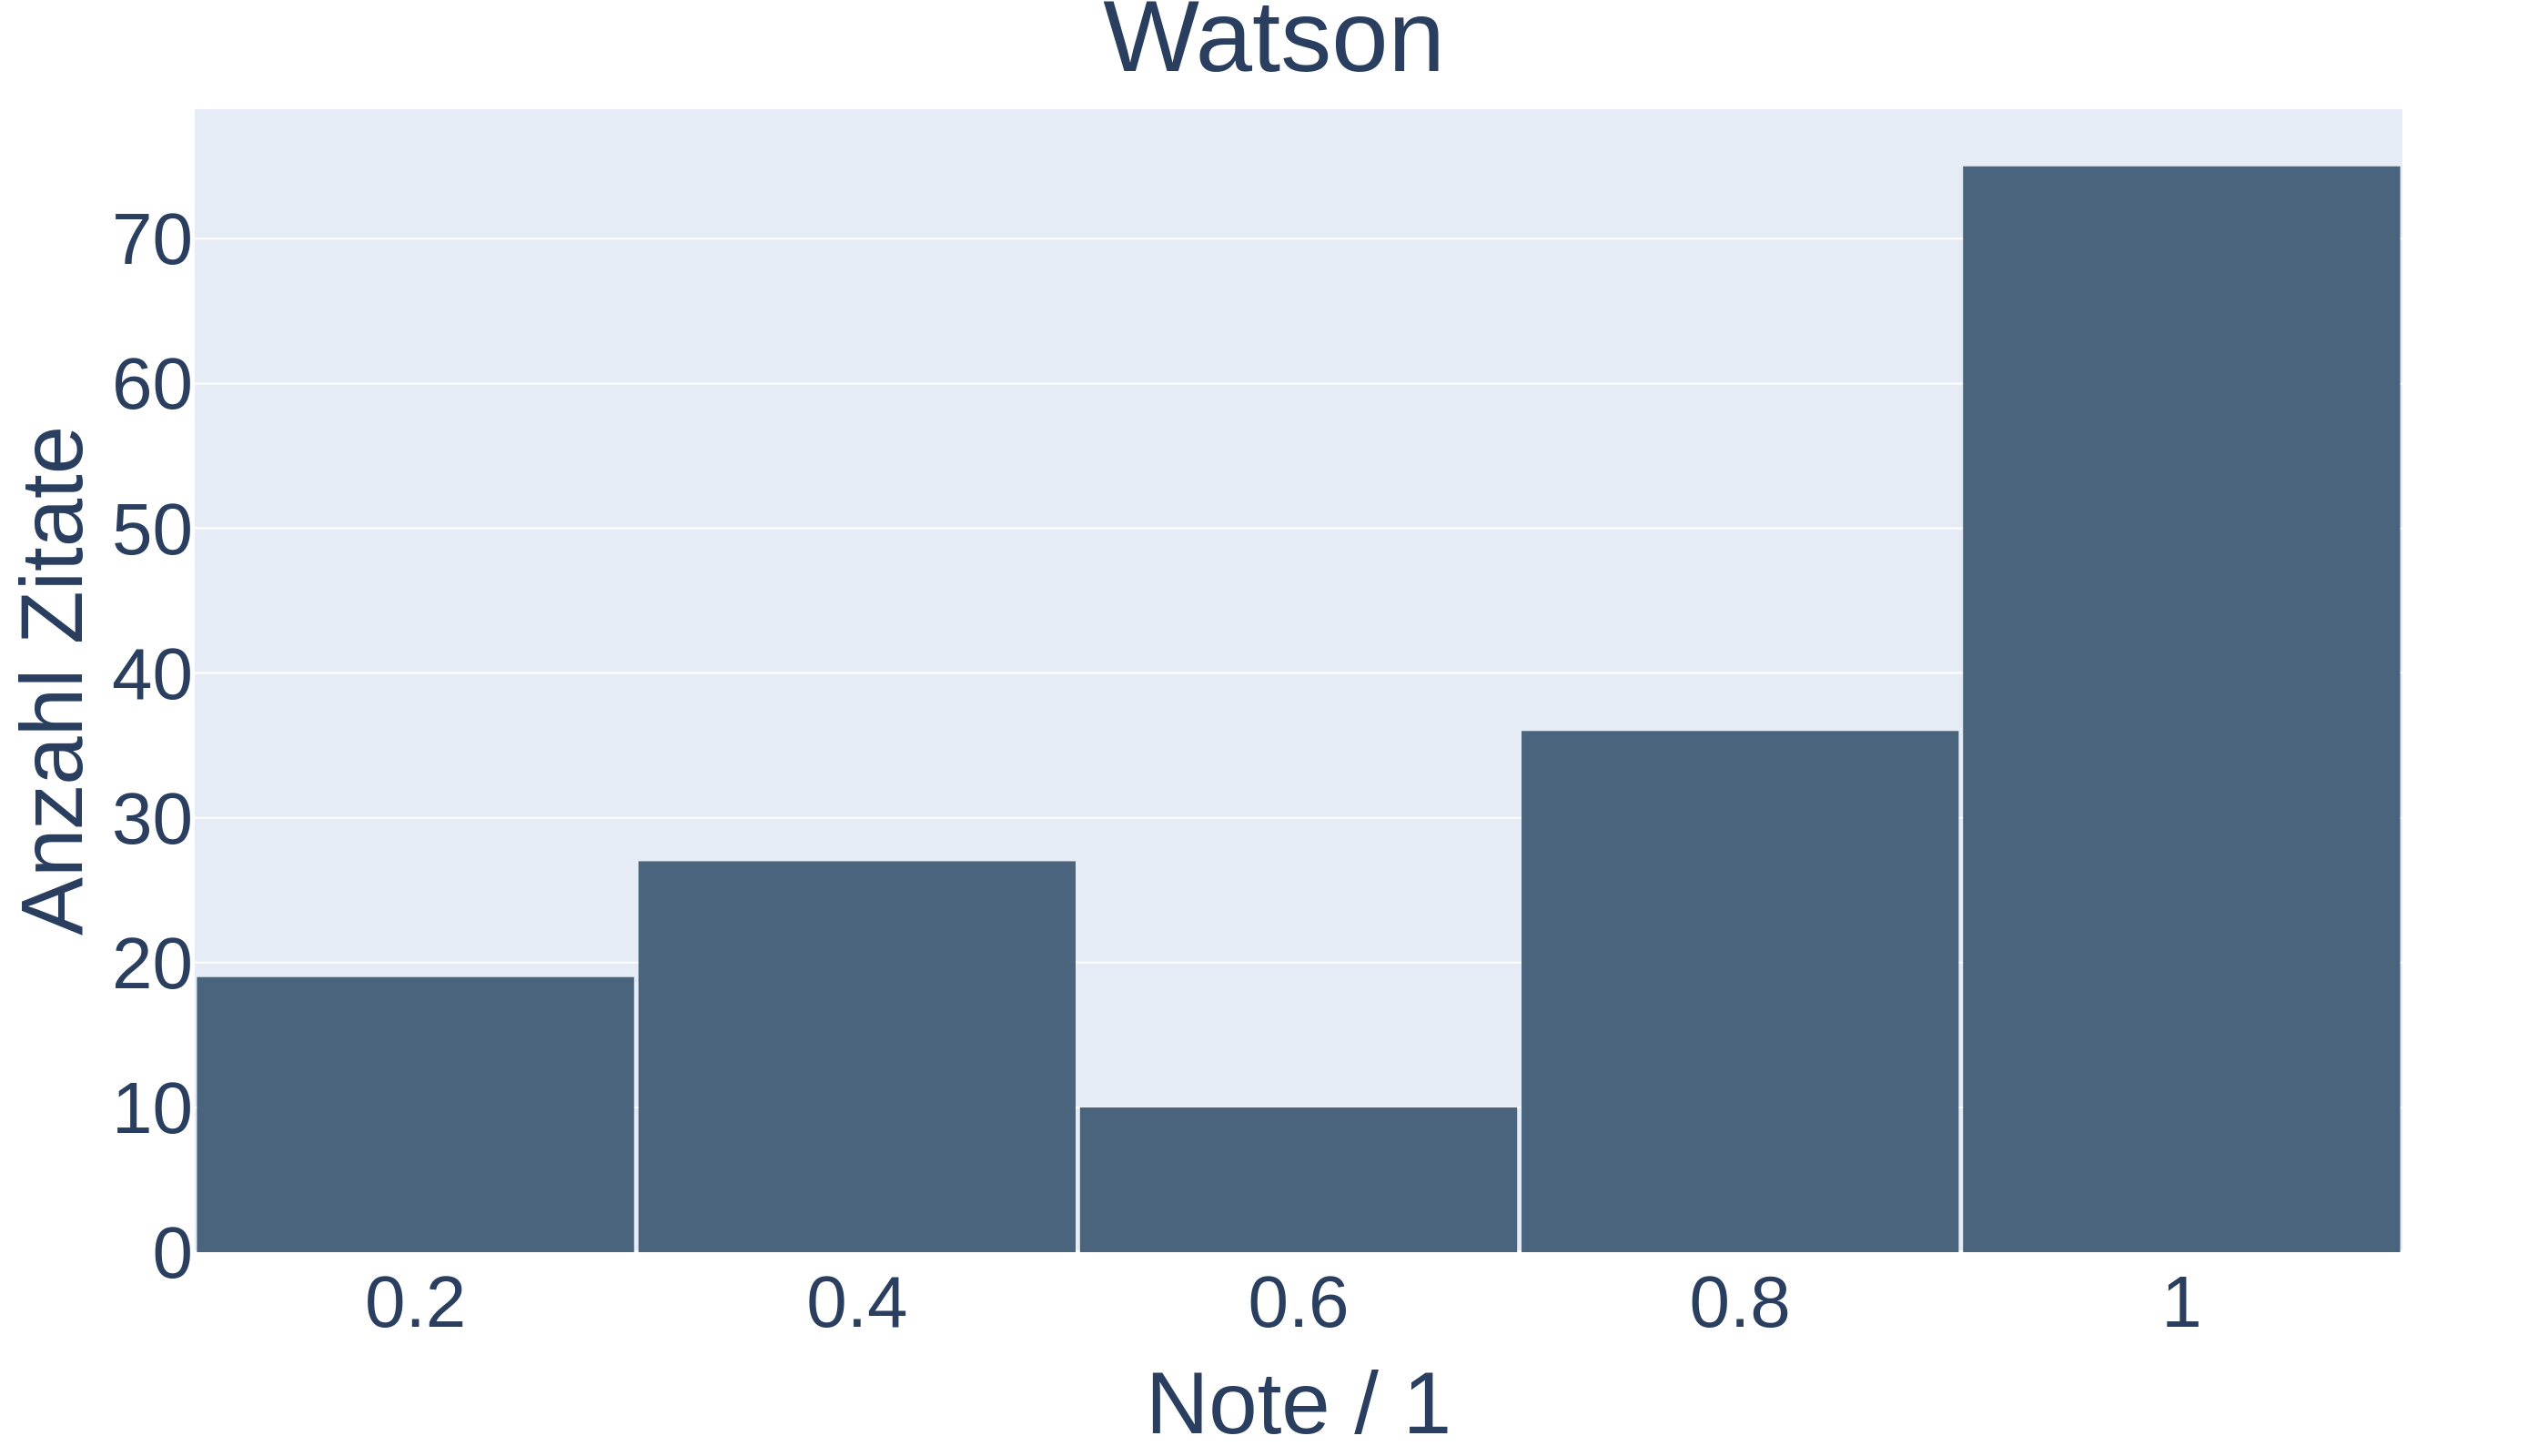
\includegraphics[width=.5\linewidth]{./images/citation_grades_watson.png} \\
	\end{tabular}
	\caption{Histogramme zur Verteilung der Qualität der gefundenen Zitate}
	\label{histogram-grades}
\end{figure}

\subsection{Nicht erkannte Zitate}\label{not-recognized-quotes}

Das nachfolgende Unterkapitel soll einen Überblick über die nicht erkannten Zitate liefern
und erklären, weshalb der Algorithmus aktuell noch nicht in der Lage ist, diese zu erkennen.

Grundsätzlich gibt es viele mögliche Erklärungen, weshalb das Programm gewisse Zitate nicht
erkennen kann. Aufgrund der analysierten Fälle scheinen die meisten fehlenden Zitate
entweder neuen, nicht implementierten Satzstrukturen oder Fehlern des Parsers geschuldet zu sein.

Es hat sich gezeigt, dass der Parser in langen Sätzen mit mehr als zwei Satzteilen
die Abhängigkeiten anders aufbaut. Deshalb wird der Subtree vom Algorithmus ignoriert.
So wird das Zitat einleitende Verb \enquote{schreibt} im folgenden Beispielsatz
als \enquote{mnr} (postnominal modifier) gekenntzeichnet (vgl. Abbildung \ref{citation-with-different-tree-structure-1}).
Wann und wie die gesuchten Verben mit diesem Label auftreten, konnten wir
nicht herausfinden.

\enquote{Dort habe er in einer Wohnung auch einen Grossteil seiner Sachen, unter anderem Familienerbstücke, wie das Inventar aus dem Restaurant Rossberg, wie der «Landbote» schreibt.}

\begin{figure}[H]
	\begin{center}
        \centering
		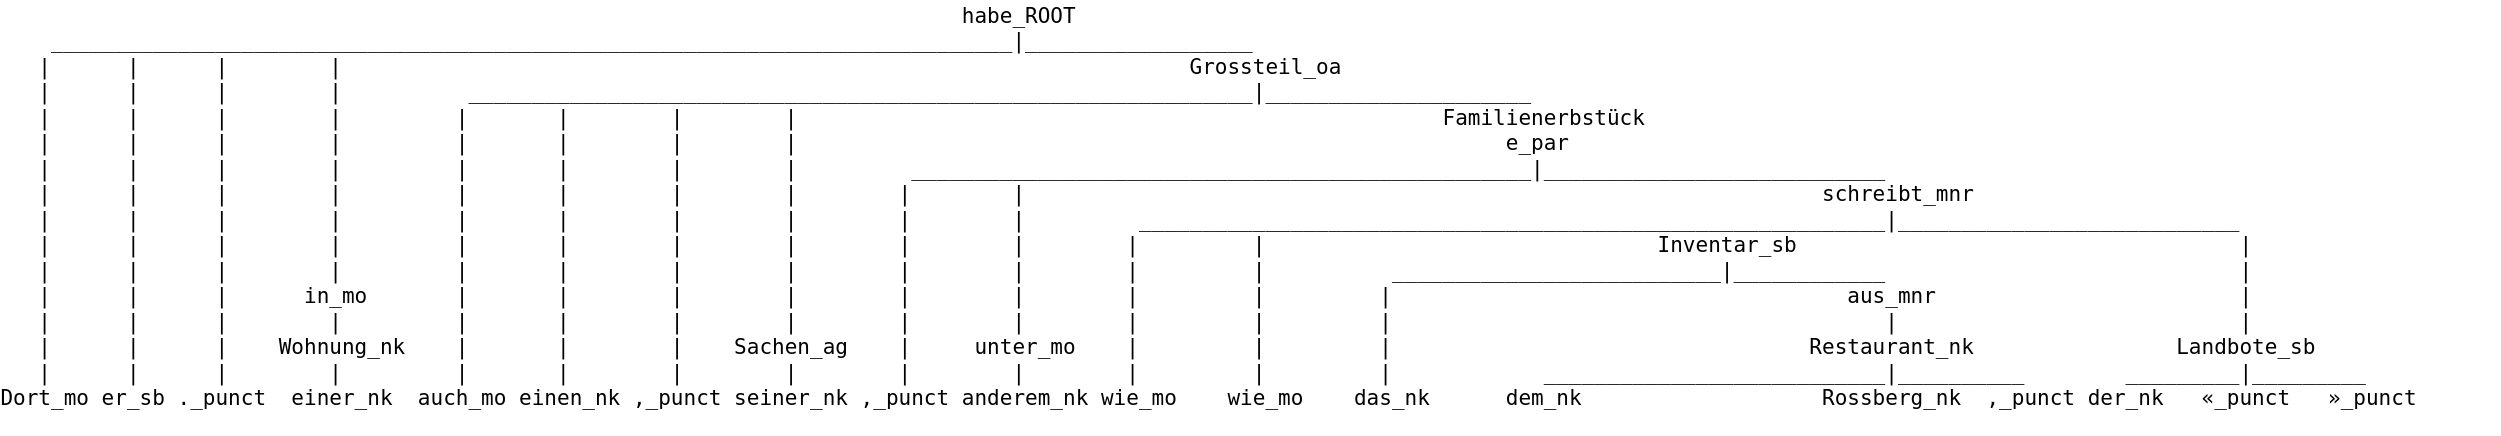
\includegraphics[width=1.0\linewidth]{./images/parse-tree-landbote.png}
	\end{center}
	\caption{Zitat mit anderer Baumstruktur}
	\label{citation-with-different-tree-structure-1}
\end{figure}

Bei dem nachfolgenden Satz wird das signifikante Verb \enquote{mitteilte} als \enquote{mo}
(modifier) gelabelt (vgl. Abbildung \ref{citation-with-different-tree-structure-2}).
In diesem Fall scheint der Parser das Label falsch vergeben zu haben,
denn \enquote{modifier}s werden meist den Adverben und Präpositionen zugeordnet.
Möglicherweise hat der Wortteil \enquote{mit} in diesem Fall den Ausschlag gegeben.

\enquote{Das Departement für Verteidigung, Bevölkerungsschutz und Sport (VBS) wird bis Ende Jahr die rechtlichen Grundlagen erarbeiten, wie der Bundesrat am Mittwoch mitteilte.}

\begin{figure}[H]
	\begin{center}
        \centering
		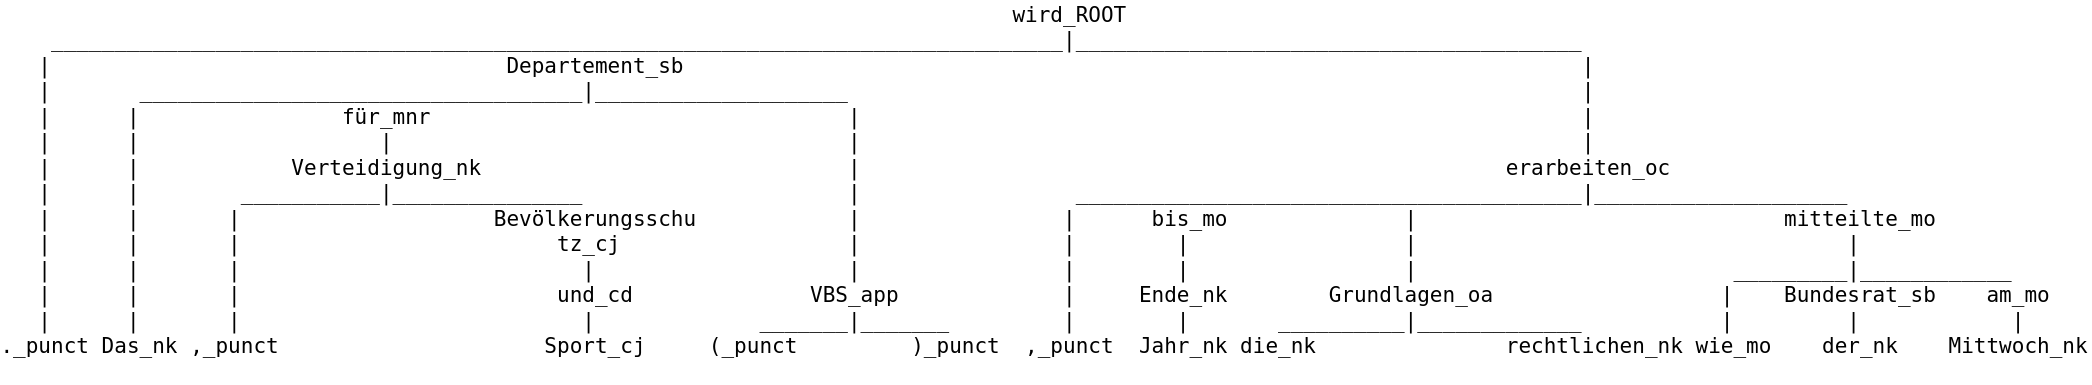
\includegraphics[width=1.0\linewidth]{./images/parse-tree-watson.png}
	\end{center}
	\caption{Zitat mit anderer Baumstruktur}
	\label{citation-with-different-tree-structure-2}
\end{figure}

\chapter{Diskussion}
%The Discussion chapter describes the consequences of your project (for the user, society, ...)
%and gives an outlook on possible next steps. You can also discuss possible limitations or
%problems that you have come across and how you handled them.

% Die Diskussion besteht aus 4 Teilen:
% Zusammenfassung der Ergebnisse
% Interpretation der Ergebnisse
% Beschränkungen der Forschung
% Empfehlung für weiterführende Forschung

 

\section {Zusammenfassung der Ergebnisse}

% Zusammenfassung der Ergebnisse

% Zu Beginn deiner Diskussion gibst du nur eine kurze Zusammenfassung deiner 
% relevanten Ergebnisse. Du solltest hier auch deine Problemstellung erneut 
% darlegen. So kannst du deine Diskussion direkt im Bezug auf dein 
% Forschungsinteresse formulieren.

Das Resultat der durchgeführten Untersuchung zeigt einen klaren und erstaunlich
gleichmässigen \gl{gendergap} in allen analysierten Nachrichtenportalen von
41.77\% bis 57.70\%. Die Ergebnisse erfüllen damit die gestellte Aufgabenstellung, indem sie
die Grösse dieses Gaps in den grössten schweizer Gratis-Online-Nachrichtenportalen
benennen.

\section {Interpretation der Resultate}\label{interpretation}

% Interpretation von Ergebnissen

% Projekt von Ringier
% Original GGT
% Does Gender Matter in the News? Detecting and Examining Gender Bias in News Articles
% A Large-Scale Test of Gender Bias in the Media
% Bezug auf Resultate von anderen Studien
% Erklärung/Vermutung des Unterschieds

% Besprich die Forschungsergebnisse und gib an, inwiefern deine Erwartungen erfüllt 
% oder nicht erfüllt wurden. Diese Erläuterungen kannst du aus deiner verwendeten 
% Literatur ableiten, sie können jedoch auch auf deinen eigenen logischen Überlegungen 
% basieren. Auf jeden Fall solltest du beschreiben, wie deine Ergebnisse in den Rahmen
% passen, den du mittels Einleitung, Theorie und Forschungsfragen sowie Hypothesen 
% aufgestellt hast. Halte ebenfalls fest, inwiefern deine Resultate neue oder andere 
% Erkenntnisse in Bezug auf dein Thema mit sich bringen. Gehe alle Möglichkeiten durch: 
% Was genau hast du herausgefunden?

Die resultierenden Ergebnisse der Untersuchung ergänzen das Bild, das von der aktuellen Forschung
gezeichnet wird (vgl. Kapitel \ref{state-of-the-art}). Der \gl{genderbias} in den Medien wurde bereits auf unterschiedlichste
Arten gemessen: anhand der Anzahl Nennungen von Frauen und Männern \cite{does-gender-matter-in-the-news},
anhand von Zitaten \cite{gender_gap_tracker}, Quellenangaben \cite{citation-network} oder absolut
vergleichbaren Paaren \cite{gender_bias_in_media}. Stets scheint der gemessene Bias, der im Endeffekt
den Unterschied im Raum misst, der den Geschlechtern in den Medien eingeräumt wird, zwischen 20\%
und 60\% zu liegen, je nach Studie.

Im Vergleich zum kanadischen \gl{ggt} \cite{gender_gap_tracker}, der die Inspiration für diese Arbeit
geliefert hat, sind die Ergebnisse ähnlich aber im Schnitt doch etwas schlechter. So lag der \gl{gendergap}
über alle Nachrichtenportale in der Arbeit \citetitle{gender_gap_tracker} bei 42\%, bei unseren Resultaten jedoch bei
50.34\%. Dies widerlegt die Vermutung, die wir in der Vorarbeit \cite{project2} auf Basis des \citetitle{gggr-20}
\cite{gggr-20} getroffen haben. Wir sind davon ausgegangen, dass der \gl{gendergap} in der Deutschschweiz
etwas geringer ausfällt, als in Kanada, weil die Schweiz im internationalen Vergleich eine deutlich bessere
Geschlechtergerechtigkeit kennt, als Kanada \cite{gggr-20}.

Die Studie \citetitle{does-gender-matter-in-the-news} \cite{does-gender-matter-in-the-news} kommt in Bezug
auf den \gl{gendergap} je nach Datensatz auf sehr unterschiedliche Ergebnisse. So weisen die Artikel aus \gl{mind}
einen Gap von 53.9\% auf, gemessen an der Anzahl Nennungen von Männern und Frauen in Abstracts von Nachrichtenartikeln.
Diese Zahl ist vergleichbar, mit dem Resultat, das wir in dieser Auswertung gefunden haben.
\gl{ncd} schneidet mit 14.5\% unter Betrachtung dieser Metrik sehr gut ab. Doch zu beachten ist bei diesem Resultat die
Verteilung der Artikel über die Kategorien. Denn in den Kategorien \enquote{Style \& Beauty}, \enquote{Parenting} 
und \enquote{Entertainment} sind Frauen deutlich übervertreten. Trotzdem ist der \gl{gendergap} in diesem Datensatz
deutlich geringer, als derjenige, den wir gefunden haben.

Auch in der Studie \citetitle{gender_bias_in_media} \cite{gender_bias_in_media} wird ein starker Bias in der Anzahl
Nennungen von Personen der unterschiedlichen Geschlechter gemessen. So liegt der \gl{gendergap} im dritten Experiment,
das Paare von Frauen und Männern im gleichen Alter, in derselben beruflichen Kategorie von gleichem öffentlichen Interesse vergleicht
bei 46.71\%. Eine grosse Zahl, jedoch immer noch etwas kleiner als derjenige, den wir gemessen haben. So scheint der
\gl{gendergap} in der Deutschschweiz insgesamt grösser zu sein als im amerikanischen und kanadischen Raum.

Recherchen zu ähnlichen Projekten in der Schweiz ergeben jedoch ein hoffnungsvolles Bild. So misst der \gl{ringier} Verlag
in seinem Projekt \gl{equalvoice} \cite{ringier-equalvoice} die Repräsentation von Männern und
Frauen in seinen Medienhäusern anhand des \enquote{Body Counts}, der Anzahl Nennungen von Männern und Frauen und hat im
Jahr 2022 einen Unterschied von noch 34.95\% festgestellt. Wobei auch hier ein grosser Unterschied bei den unterschiedlichen Zeitungen
feststellbar ist. So schneidet die Print Ausgabe von Blick mit 42\% auch in dieser Auswertung ähnlich schlecht ab, wie
in den vorliegenden Resultaten mit 49.59\%. Es ist jedoch zu beachten, dass das Resultat von \gl{equalvoice} nur das Jahr 2022
betrifft und unsere Auswertung jedoch bis ins Jahr 2004 zurückreicht. Leider ist auf der Webseite auch zu erkennen, dass
sich der \gl{gendergap} seit dem Ende der Coronapandemie wieder weitet. \citeauthor{gender_gap_tracker} mutmassen in ihrer Arbeit,
dass dies auf den reduzierten Fokus auf dem von Frauen dominierten Gesundeheitsbereich zurückzuführen ist \cite{gender_gap_tracker}.
Es ist spannend, zu erkennen, dass diese Veränderung sowohl in Kanada wie auch in der Schweiz die gleichen Effekte zu haben scheinen.

Obwohl der sich der \gl{gendergap} wieder etwas geweitet hat, ist es jedoch höchst erfreulich, dass sich die Verlage zunehmend Gedanken zu diesem Thema machen und Lösungen anstreben.
So hat uns SRF bei unserer Anfrage nach einer Stellungnahme darauf hingewiesen, dass sie beispielsweise in der beliebten schweizer Radiosendung 
\enquote{Echo der Zeit} \footnote{https://www.srf.ch/audio/echo-der-zeit} im Februar erstmals mehr Gesprächspartnerinnen
als Gesprächspartner in den Echo-Gesprächen hatten \footnote{Dieser Beitrag konnte öffentlich nicht gefunden werden.}.
Es scheint als wären sich zumindest SRF und Ringier (Blick Mutterkonzern) der Problematik bewusst zu sein und Aufwand zur
Verringerung des \gl{gendergap}s zu betreiben. Trotzdem scheint die Deutschschweiz auf diesem Gebiet im Vergleich mit
den amerikanischen und kanadischen Nachrichtenportalen hinterherzuhinken und noch viel Arbeit betreiben zu müssen, um
den Unterschied weiter zu verkleinern.

Unter dieser Betrachtung stellt sich auch die Frage, was die Ursachen für dieses Problem sind.
So zeigt beispielsweise die Arbeit \citetitle{gender_bias_in_media} \cite{gender_bias_in_media} auf,
dass dieser Bias nicht alleine durch eine Präferenz der Medienschaffenden zur Porträtierung von Männern zustande kommt,
sondern auch der Struktur unserer Gesellschaft geschuldet ist, in der ein Grossteil der nachrichtenwerten
Positionen von Männern belegt wird. Dies ist nicht zuletzt dem Phänomen des \gl{glass-ceiling} geschuldet,
wie verschiedene Studien zeigen \cite{glass_ceiling_effect,glass_ceiling_politics}.

Die Bereinigung dieser Ungerechtigkeit kann also nicht von den Medienschaffenden alleine gelöst werden, denn
ihre Aufgabe in unserer Gesellschaft besteht in erster Linie in der Informationsverbreitung und der Schaffung
von Transparenz in den für die Öffentlichkeit interessanten Bereichen. Trotzdem können sie durch bewusste und reflektierte
Berichterstattungen und Recherchen ihren Anteil am Problem verringern und so die Gesamtsituation verbessern.
Die eigentliche Herkulesaufgabe, die Transformation unserer Gesellschaft zu einer ausgeglicheneren und
faireren Zivilisation, wird jedoch noch viel Effort von der Politik, Wirtschaft und jedem und jeder einzelnen von uns erfordern. % :)

\section {Limitationen}\label{limitations}

% Begrenzungen (limitations) deiner Untersuchung

% Die Begrenzungen bzw. Limitationen deiner Arbeit – im Englischen ‚limitations‘ 
% – erörterst du in einem eigenen Absatz innerhalb der Diskussion deiner Bachelorarbeit 
% bzw. Masterarbeit. Hier gehst du darauf ein, inwiefern du bei deiner Forschung an
% Grenzen gestoßen bist und welche Auswirkungen sich auf deine Ergebnisse ergeben haben.
% Wenn es ein paar Randbemerkungen zu deiner Forschung gibt oder du bestimmte
% Limitationen stark zu spüren bekommen hast, können diese auch eine Erklärung für deine
% Endresultate sein. Du kannst z. B. angeben, ob Fragen offen geblieben sind und auf
% Basis deiner Resultate Empfehlungen für zukünftige Forschung aussprechen. Achte 
% jedoch darauf, dass du deine eigene Forschung nicht gänzlich schlechtredest: Es ist
% nicht das Ziel, dass du eine Zusammenfassung aller kleinen Fehler erstellst. Über
% diese hättest du bereits nachdenken müssen, bevor du mit deiner Forschung angefangen
% hast.
Die Aufgabe, Zitate aus natürlichem Text zu extrahieren, ist eine schwierige. Die
menschliche Sprache kennt unzählige Wege, wie die Botschaft einer Person wiedergegeben
werden kann. Die Botschaft und die Tatsache, dass sie von einer anderen Person wiedergegeben wird,
ist durch die Syntax des Textes und den Kontext gegeben. \citeauthor{gender_gap_tracker} haben in
ihrer Arbeit \cite{gender_gap_tracker} zwei Arten von Zitaten identifiziert, für welche sie unterschiedliche
Herangehensweisen in ihrem Parsingprozess definierten. Doch auch sie konnten aufgrund der Regelmässigkeiten dieser
zwei Typen nicht alle Zitate herausfiltern und mussten auf heuristische Methoden zurückgreifen,
um übriggebliebene Zitate erkennen zu können. Die Struktur natürlichen Textes ist ambiguös und dessen Bedeutung
kontextabhängig. Obwohl gängige \gl{ml} gestützte
\gl{nlp}-Werkzeuge wie \gl{spacy} heute besser sind, diese Eigenschaften zu erkennen und einzuordnen,
scheinen die Resultate nur in einfachen Satztstrukturen zuverlässig zu funktionieren, wie unsere
Erfahrungen zeigten (vgl. Kapitel \ref{not-recognized-quotes}). So war es für uns in der kurzen Zeit
leider nicht möglich, den Prozess der Zitat-Extraktion zu verfeinern und um weitere Zitattypen zu erweitern.
Diese Einschränkung hat den grössten Einfluss auf die Qualität der vorliegenden Resultate.

Das bedeutet, dass wir schätzungsweise 60\% der gängigsten \textsl{Syntaktischen Zitate} gefunden haben. Diese Schätzung
basiert auf der Annahme, dass unsere Testresultate ein zuverlässiges Bild über die Performance auf den
restlichen Daten abgeben. Da es neben den \textsl{Syntaktischen Zitaten} auch noch die \textsl{Schwimmenden Zitate} gibt,
stellen diese nur einen Teil der Gesamtmenge der Zitate dar.
Ohne genauere Angaben zu der Verteilung der Anzahl Zitate auf deren
unterschiedlichen Kategorien zu kennen, schätzen wir den Anteil der \textsl{Syntaktischen Zitate} auf etwa 50\%.
Denn \textsl{Schwimmende Zitate} kommen unbegleitet von \textsl{Syntaktischen Zitaten} eigentlich nicht vor,
weil sonst der Kontext fehlen würde und die lesende Person keine Informationen zum Subjekt hätte.
Doch wenn sie vorkommen, treten sie meist in grösseren Mengen auf (bspw. in längeren Interviews).
Unter der Annahme, dass die verwendeten Tests ein repräsentatives Bild der Performance
des Algorithmus abgeben und dass die oben beschriebene Schätzung korrekt ist, hat das Programm
60\% von 50\%, also insgesamt 30\%, aller Zitate erkannt.
Es könnte also theoretisch sein, dass diejenigen 70\% der Zitate, die wir nicht erkannt haben, hauptsächlich von
Frauen sind. Dann hätten wir einfach "Pech" gehabt, dass der Algorithmus mit seiner Methode hauptsächlich Zitate
von Männern extrahiert, obwohl das Verhältnis effektiv anders wäre.
Aufgrund der grossen Datenmenge und der
Ergebnisse anderer Studien und Projekte glauben wir, dass dem nicht so ist und unsere Ergebnisse einen tatsächlichen
\gl{gendergap} in den deutschschweizer online-Medien widerspiegeln.
Doch mit Sicherheit lässt sich dies nicht sagen.

Die verwendeten Werkzeuge verfügen ihrerseits über Ungenauigkeiten. So gibt \gl{spacy} für das
von uns verwendete Model \enquote{Accuracy Scores} von > 90\% an \footnote{https://spacy.io/models/de\#de\_core\_news\_lg-accuracy}.
Für das \gl{pos} Tagging wird eine Präzision von 98\% versprochen und für das gelabelte 
\gl{dependency-parsing} eine von 91\%.
Auch bei der Erkennung der Personen herrscht eine gewisse Unsicherheit durch die
probabilistische Natur des \gl{spacy} Modells. So verkündet die offizielle Webseite zwar
eine Accuracy von 98\%, doch nach unserer Erfahrung ist zumindest die Anzahl von False-Positives
deutlich höher. Wir konnten beobachten, dass die Entitäten
zwar erkannt wurden, jedoch unter einem falschen Label. Meist waren dies Organisationen oder Orte,
die \gl{spacy} als Personen identifiziert hatte. Leider konnten wir nicht herausfinden,
welche Metrik \gl{spacy} für die Messung der Accuracy verwendet. Aufgrund der subjektiven
Erfahrung gehen wir aber davon aus, dass es sich wohl um eine Metrik handeln muss, die
False-Positives nicht oder nur schwach berücksichtigt. So könnte es sich bspw. um den \gl{recall}
handeln.

\section{Weiterführende Forschung}\label{further-research}

% Empfehlungen für weiterführende Forschungen

% Die Diskussion deiner Bachelorarbeit bzw. Masterarbeit kann mit einem Absatz zu 
% Empfehlungen für eventuell weiterführende Forschungen enden. Wie können andere 
% Forschende auf deiner Forschung aufbauen? Wo ergeben sich Ansatzpunkte für weitere 
% Untersuchungen? Vermeide Aussagen im Stil von ‚Es wird noch viel Forschung nötig sein‘. 
% Es ist nicht das Ziel, dass andere sich Ergänzungen zu deiner Arbeit überlegen müssen.
% Nenne ein paar konkrete Vorschläge für unabhängige weiterführende Untersuchungen,
% denen deine Arbeit als Orientierung dienen kann.

Die Resultate legen nahe, dass in den untersuchten Nachrichtenportalen ein grosser
\gl{gendergap} herrscht. Der zeitliche Rahmen hat jedoch weiterführende Untersuchungen
und Qualitätsverbesserungen verhindert. So bestünde der erste Schritt der weiterführenden Forschung
wohl darin, die Qualität der Ergebnisse zu verbessern und mit weiteren Tests sicherzustellen.
Dazu könnten weitere Testfälle manuell definiert werden für die \textsl{Syntaktischen Zitate}.

Ein weiterer wichtiger Punkt wäre die Extraktion der \textsl{Schwimmenden Zitate} mit entsprechenden
Test Sets. Erst wenn auch diese zu einem zufriedenstellenden Teil analysiert werden, kann eine abschliessende
Aussage zum \gl{gendergap} in den deutschschweizer online-Medien getroffen werden.

Weiterhin wäre es spannend zu erfahren, wie gross der Unterschied in den unterschiedlichen Kategorien von Nachrichtenartikeln ist.
Diese Erkenntnisse könnte man in Vergleich setzen
mit der Arbeit \citetitle{gender_bias_in_media} \cite{gender_bias_in_media} von \citeauthor{gender_bias_in_media} oder
dem Paper \citetitle{does-gender-matter-in-the-news} von \citeauthor{does-gender-matter-in-the-news}.
Des Weiteren wäre von Interesse, welcher Anteil der strukturelle Bias in unserer Gesellschaft
an diesem Gap hat und welcher Anteil dem Bias in der Berichterstattung von Medienschaffenden
geschuldet ist. Dazu könnten interessierte Forschende eine ähnliche Methodik wie
\citeauthor{gender_bias_in_media} in \citetitle{gender_bias_in_media} \cite{gender_bias_in_media}
anwenden.

Eher moralischer Natur ist die Forschungsfrage, ob dieser Gap überhaupt etwas
Schlimmes ist. Die Antwort zu dieser Frage liegt wohl in der Meinung der von
dieser Tatsache diskriminierten Gruppe, der Frauen. Hierzu könnte eine Meinungsumfrage
Aufschluss bieten.

Interessant wäre auch zu wissen, welche Auswirkungen sich aus diesem Gap ergeben.
Es ist unbestritten, dass Medien die Meinung einer Gesellschaft prägen. So kann
wohl auch angenommen werden, dass die Unterrepräsentation der Frauen in den Medien
Nachteile für diese mit sich bringt. Wie diese Nachteile aussehen, die sich aufgrund
dieser Unterrepräsentation ergeben, lässt sich aufgrund des aktuellen Forschungsstands
nicht sagen. Obwohl die strukturellen Benachteiligungen der Frauen gegenüber den Männern
klar benennbar sind, ist es schwierig diese auf einzelne Ursachen zurückzuführen. 
Weiterführende Forschung könnte hier Klarheit schaffen.


% \chapter{Schlussfolgerungen}
%The Conclusion sums up the results of the project. You should also state your personal
%learnings in the project here.

\chapter{Schlussfolgerungen}

% Das Fazit steht im direkten Zusammenhang mit der Einleitung, 
% da du auf die Forschungsfragen oder Hypothesen eingehst, 
% die zu Beginn der Bachelorarbeit aufgestellt wurden.

% Im Fazit deiner Bachelorarbeit wiederholst du nicht noch einmal die gesamte Arbeit,
% sondern du legst zusammenfassend die wichtigsten und aussagekräftigsten Ergebnisse dar. 
% Beim Schreiben des Fazits solltest du also die folgenden Regeln beachten:

%     Keine neuen Informationen und Interpretationen
%     Das Fazit ist grundsätzlich eine Zusammenfassung deiner wichtigsten Erkenntnisse. 
%     Es darf daher nur mit Informationen und Gedankengängen gefüllt werden, die du bereits im Fließtext dargelegt hast.
%     Keine Beispiele und Zitate
%     Im Fazit fasst du Fakten zusammen und erklärst sie nicht anhand neuer Beispiele und Zitate anderer Forschenden.
%     Dein Ergebnis ist immer wertvoll
%     Es kann vorkommen, dass deine Ergebnisse nicht deinen Erwartungen entsprechen. 
%     Wenn du deine Forschungsfrage aber gut gestellt hast, bspw. mit den Formulierungen‚
%     wie viel‘ oder ‚inwiefern‘, wirst du immer ein wertvolles Ergebnis erhalten, 
%     das die Forschung auf diesem Gebiet weiterbringt.


% Ziele der Arbeit (aus der Einleitung):
% Die Arbeit soll aufzeigen, inwiefern das Erkennen von Zitaten
% mittels \gl{nlp} Werkzeugen auch in deutschsprachigen Texten möglich ist. Anhand dessen
% soll sie analysieren, wie viele der gefundenen Zitate von Männern sind und wie viele von Frauen.

\section{Evaluation der Ziele}

Die vorliegende Arbeit hatte zwei grosse Ziele. Beide sind zuvor noch nie umgesetzt worden,
sofern wir das ermitteln konnten.

\begin{itemize}
    \item Die Arbeit sollte aufzeigen, inwiefern das Erkennen von Zitaten mittels \gl{nlp} Werkzeugen auch in deutschsprachigen Texten möglich ist.
    \item Sie sollte den \gl{gendergap} anhand der Anzahl Zitate von Männern und Frauen in den gesammelten Texten bestimmen
    und diesen mit den verwandten Arbeiten vergleichen.
\end{itemize}

Aus diesen zwei Hauptzielen ergaben sich Zwischenziele, die wir ebenfalls festhalten möchten.
Das erreichen dieser Zwischenschritte war essenziell für das Bestimmen des \gl{gendergap}s.
\begin{itemize}
    \item Der Algorithmus zum Bestimmen des Gender Gaps muss Personen und dazugehörige
    Informationen aus den Artikel Texten extrahieren können.
    \item Die Software soll in der Lage sein, das Geschlecht der identifizierten Personen zu bestimmen.
\end{itemize}

\subsection{Erkennen der Zitate}

Mithilfe des erstellten Programms konnten wir zeigen, dass das Erkennen von Zitaten mithilfe von \gl{nlp} Werkzeugen
auch in deutschschweizer online-Artikeln möglich ist. So konnte der Algorithmus in einem Datensatz
mit 351'021 einzigartigen Artikeln 133'443 Zitate extrahieren.

Innerhalb von zwei Wochen war es uns
möglich, schätzungsweise 60\% aller \textsl{Syntaktischen Zitate} zu extrahieren.
Wir sind überzeugt, dass mithilfe eines grösseren Testsets und Verfeinerungen des Algorithmus
eine höhere Präzision und Verlässlichkeit der Extraktion der \textsl{Syntaktischen Zitate} möglich ist.
Darauf aufbauend sollte auch die Erkennung der \textsl{Schwimmenden Zitate} möglich sein, vermuten wir.
Um eine verlässliche Aussage bezüglich des \gl{gendergap}s treffen zu können, müssten diese Verbesserungen und Erweiterungen unbedingt durchgeführt werden.

\subsection{Ermitteln des Gender Gaps}

Das Resultat der durchgeführten Analyse zeigt einen \gl{gendergap} von 50.34\% über alle Zitate auf.
Der grösste gemessene Gap pro Nachrichtenportal liegt bei 57.7\%, der kleinste bei 41.77\%.
Die Datengrundlage für diese Auswertung bildet ein bereinigtes Datenset von 351'021 einzigartigen
deutschsprachigen online-Artikel aus vier Nachrichtenportalen der Deutschschweiz. Die Analyse umfasst
schätzungsweise 60\% aller \textsl{Syntaktischen Zitate} und 30\% aller Zitate insgesamt.

Die gemessenen Unterschiede in der Anzahl Zitate lassen sich mithilfe der von uns definierten
\gl{gendergap} Formel (vgl. Abbildung \ref{ggt-formula}) mit anderen Arbeiten vergleichen.
Der direkteste Vergleich lässt sich mit dem \enquote{Body Count} von Blick aus der \gl{equalvoice}
Initiative anstellen. Die Print Ausgabe misst dabei einen \gl{gendergap} von 42\%, während unsere
Daten für das online Portal einen Gap von 49.59\% anzeigen.
Die Vorbildsstudie \citetitle{gender_gap_tracker} \cite{gender_gap_tracker} misst in den kanadischen Medien
einen \gl{gendergap} von 42\%.
\citetitle{does-gender-matter-in-the-news} \cite{does-gender-matter-in-the-news}
misst je nach Datensatz einen \gl{gendergap} von 53.9\% oder 14.5\%.
\citetitle{gender_bias_in_media} \cite{gender_bias_in_media} kann einen \gl{gendergap} von 46.71\% nachweisen.

Die berechneten \gl{gendergap}s der verwandten Arbeiten zeichnen ein ähnliches Bild, wie jenes
der vorliegenden Resultate. Es scheint als würde sich der Unterschied im Raum, der Männern
und Frauen zugesprochen wird - mit Ausnahmen natürlich - im Bereich von etwa 40\% - 50\% bewegen.

\subsection{Extraktion der Personen}
Die Kombination von \gl{ner} und \gl{cr} ermöglichte eine weitgehende Extraktion und Identifizierung 
der im Text genannten Personen. 
Durch den Einsatz dieser beiden Verfahren konnten die Personen grundsätzlich erfolgreich aus dem Text herausgefiltert werden.

Dennoch ist es wichtig zu betonen, dass die Extraktion von Personen aus Texten keine absolute Gewährleistung für eine fehlerfreie Identifizierung bietet. 
Es besteht immer die Möglichkeit von Fehlern, insbesondere wenn die Namen mehrdeutig sind, wenn im 
Text Unklarheiten auftreten oder Verweise auf nicht eindeutige Personen gemacht werden.

\subsection{Bestimmen des Geschlechts einer Person}
Das Geschlecht konnte bei 87.2\% aller gefundenen Personen, denen ein Zitat zugewiesen wurde, erfolgreich bestimmt werden. 
Die restlichen 12.8\% der Personen, bei denen das Geschlecht nicht ermittelt werden konnte, sind entweder vermutlich keine 
tatsächlichen Personen, da sie fälschlicherweise vom \gl{ner} als solche erkannt wurden, oder es handelt sich um Namen, 
denen kein eindeutiges männliches oder weibliches Geschlecht zugeordnet werden können.

Wir hatten auch die Idee, das Geschlecht der Autorinnen und Autoren der Artikel zu bestimmen. 
Leider war die Datenqualität der vorliegenden Datengrundlage aus dem Vorgängerprojekt unzureichend. 
Oftmals waren im Feld \enquote{author} der Datenbank keine Namen, sondern nur unbrauchbare Daten enthalten.
Wir vermuten, dass Teile des Artikels als Autor:in erkannt wurden, 
da die Autorinnen und Autoren Informationen häufig am Ende des Texts in einer nicht eindeutigen Form aufgeführt wurden.


\section{Persönliche Erkenntnisse}

\subsection{Literaturrecherche}
% Viel Hilfe von Frau Kurpicz zu Beginn der Phase beim Definieren der Methode
% Wir hatten genug vom Lesen und Zusammenfassen
% Wir waren ungeübt und mussten das Literatur-Analysieren erlernen (war schwierig)

Zu Beginn der ersten Phase unserer Arbeit, der Literaturrecherche, hatten wir das Glück, das Prof. Dr. Mascha Kurpicz-Briki uns bei der Definition unserer Forschungsmethode unterstützte. 
Sie half uns eine geeignete Methode für die Literaturrecherche zu entwickeln. 
Ihre Anleitung und Erfahrung waren sehr hilfreich und führten uns in eine richtige Richtung.

Während der Literaturrecherche hatten wir mit einer beträchtlichen Menge an wissenschaftlicher Literatur zu tun. 
Das Lesen und Zusammenfassen von zahlreichen Papers wurde mit der Zeit anstrengend und ermüdend. 
Es war eine Herausforderung, die Konzentration aufrechtzuerhalten und gleichzeitig den Überblick über die wichtigsten Informationen zu behalten.

Das Analysieren der gefundenen Literatur stellte eine neue und herausfordernde Aufgabe dar. 
Wir waren ungeübt in diesem Bereich und mussten uns mit den grundlegenden Techniken des Literatur-Analysierens vertraut machen. 
Es erforderte Zeit und Mühe, die verschiedenen Ansätze zur Bewertung und Zusammenfassung von Forschungsergebnissen zu erlernen. 
Es gab Momente, in denen es frustrierend war. Mit der Zeit und Übung konnten wir unsere Fähigkeiten verbessern.
Wir haben gelernt, dass Ausdauer und Organisation essenziell sind, um mit der Fülle an Informationen umzugehen. 

\subsection{Programmieren}
% Spass am programmieren
% Mehr Zeit als geplant für Date Bereinigung und Umgang mit dieser grossen Datenmenge (Skript Aggregation 40h)

Nach der Literaturrecherche haben wir festgestellt, dass es für uns wichtig ist, Spass am Programmieren zu haben und nicht ausschliesslich mit 
dem Lesen und Dokumentieren von Papers beschäftigt zu sein. 
Umso mehr hatten wir Freude aktiv zu programmieren und Lösungen zu entwickeln, die einen Mehrwert für unsere Arbeit bieten.
So konnten wir unsere Motivation und Kreativität aufrechterhalten, weil in der letzten Phase der Fokus dann wieder auf dem Dokumentieren liegt. 

Des Weiteren haben wir festgestellt, dass die Bearbeitung grosser Datenmengen mehr Zeit in Anspruch nehmen kann, als ursprünglich geplant. 
Insbesondere die Datenbereinigung erforderte viele Stunden bis alle Daten verarbeitet waren. 
Oftmals zwischen 20 und 30 Stunden pro Nachrichtenportal. 
Teilweise sogar mehrmals, da wir Fehler im Script bemerkten und diese nochmals neu starten mussten.
Bei der Aggregation waren auch 40 Stunden erforderlich, um alle Daten korrekt zu verarbeiten. 
Für zukünftige Projekte würden wir dies bei der Zeitplanung mehr berücksichtigen und ausreichend Zeit für die Datenbereinigung und Aggregation einplanen.

Insgesamt betrachtet war das Programmieren mit Python für uns der beste Teil der Arbeit, da wir immer wieder neue Herausforderungen und Lernmöglichkeiten entdeckten. 

\subsection{LaTeX}
% Vorkenntnisse mit LaTeX vom Projekt 2 waren Hilfreich

Unsere Vorkenntnisse in LaTeX aus Project 2 waren äusserst hilfreich. 
Sie haben uns ermöglicht, effizient mit unserem LaTeX-Dokument umzugehen und ansprechende Ergebnisse zu erzielen.

Dank unserer vorhandenen LaTeX-Kenntnisse konnten wir mit geübter Hand neue Kapitel erstellen, Formatierungen anpassen und Inhalte strukturieren. 
Wir waren mit den grundlegenden Befehlen und Konzepten vertraut, was uns geholfen hat, uns auf den Inhalt unseres 
Dokuments zu konzentrieren, anstatt viel Zeit mit dem Erlernen der grundlegenden Syntax zu verbringen wie im Vorprojekt.

\subsection{MongoDB}
Auch mit MongoDB hatten wir hilfreiche Erfahrungen aus dem Vorprojekt.
Die integrierte Abfragesprache \enquote{MongoDB Query Language} war uns auch schon bekannt und so konnten wir viel wirksamere Abfragen machen und
deren Komplexität steigern.

\subsection{Projektplanung}
% Es war schwiereig so detailiert zu planen im Voraus, aus dem Vorprojekt hatten wir nur auf Wochenbasis geplant.
% Zeitplan im grobben eingehalten
% Task von Datenbereinigung war am Anfang nicht fest eingeplannt und kahm noch dazu
% Sprint Board pro Projektphase half die Übersicht zu behalten vom Stand der Arbeiten
% Das Schreiben von Besprechungs Protokollen hat uns bei der Nachvollziehbarkeit von Entscheidungen geholfen und bei der Ausführung der Aufträge unterstützt

Im Vergleich zum Vorprojekt war es herausfordernd, die Planung im Voraus so detailliert durchzuführen. 
In diesem hatten wir hauptsächlich auf Wochenbasis geplant, doch während der Bachelor Thesis ist ein umfassender Projektplan Teil der Bewertung. 
Das Festlegen von konkreten Aufgaben und Meilensteinen auf langfristiger Basis erforderte eine sorgfältige Abwägung und eine genaue 
Einschätzung der Aufwände.

Trotz der Komplexität der Projektplanung konnten wir den Zeitplan im Grossen und Ganzen einhalten (vgl. Abbildung \ref{gantt}). 
Dies war ein Erfolg, da es uns ermöglichte, die Fortschritte des Projekts zu steuern und sicherzustellen, dass wir die gesetzten Ziele 
erreichen können. 
Die Disziplin und Organisation beider Teammitglieder trugen dazu bei, dass wir den Überblick über die Arbeitsauslastung behielten und  
unsere Deadlines einhielten.
Die Verwendung eines Sprint Boards (vgl. Abbildung \ref{sprint-board-screenshot}) für jede Projektphase erwies sich als äusserst hilfreich. Es ermöglichte uns den Fortschritt der Aufgaben zu überblicken. 
Das Sprint Board ermöglichte uns, Aufgaben zu visualisieren, den Status jedes Tasks zu verfolgen und Engpässe oder Verzögerungen frühzeitig zu erkennen. 
Dadurch konnten wir flexibel auf Änderungen reagieren und die Prioritäten entsprechend anpassen.

In unserer Projektplanung war die Datenbereinigung nicht als einzelner Task vorgesehen. 
Es stellte sich jedoch heraus, dass dieser Task erforderlich war, um mit den gesammelten Daten arbeiten zu können. 
Das Hinzufügen dieses zusätzlichen Tasks brachte eine gewisse Herausforderung mit sich, da wir unsere Zeitplanung und 
Ressourcen neu anpassen mussten, um diese Aufgabe bewältigen zu können.

Das Schreiben von Besprechungsprotokollen erwies sich als wertvoll für die Nachvollziehbarkeit von Entscheidungen und die Umsetzung von Tasks. 
Die Protokolle von den Meetings mit Prof. Dr. Mascha Kurpicz-Briki sowie von den Besprechungen mit uns beiden halfen uns, wichtige Informationen und Diskussionsergebnisse festzuhalten. 
Ausserdem war es hilfreich sicherzustellen, dass alle Teammitglieder über den Stand der Dinge informiert waren und die vereinbarten Aufgaben richtig ausgeführt wurden.

\subsection{Zusammenarbeit in der Gruppe}
% Eingespieltes Teamwork durch Projekte die wir schon vorher zusammengemacht haben
% Feedback von Frau Kurpicz kam rasch und Kommunikation mit Ihr war gut
% "Hit The Ground Running" --> Von Anfang an voll dran
% Gute Aufteilung der Arbeit in Arbeitstakte so das wir je nach Aufgaben parallel daran arbeiten konnten
% Gegenseitiges Review war effizient
% Schwierigkeiten im Team besprochen und Lösungen gefunden z.B. das wir nur Syntaktische Zitate extrahieren
% Klassische Geschlechterrollen in der Projekt Zusammenarbeit identifiziert und verändert so das wir uns abwechslen mit Präsentatieren und der Meeting-Leitung
% Meetings mit Dozentin immer recht speditiv, zeitlicher rahmen eingehalten und meistens unter den abgaemachten 30min, regelmässiger Austausch
% Spontane Terminfindung hat nicht immer funktioniert --> Lösung: Regelmässiger Termin (ab Phase Praxisteil)

Bei unserer Selbstreflexion zur Zusammenarbeit in der Gruppe haben wir folgende wichtige Erkenntnisse gewonnen:

\begin{itemize}
    \item \textbf{Eingespieltes Teamwork durch vorherige Projekte:} Dank unserer vorherigen Zusammenarbeit in anderen Projekten konnten wir als Team gut zusammenarbeiten. Wir kannten bereits unsere Stärken und Schwächen und wussten, wie wir effektiv kommunizieren und unsere Aufgaben koordinieren können.
    \item \textbf{Schnelles Feedback von Prof. Dr. Mascha Kurpicz-Briki und gute Kommunikation:}  Das rasche Feedback unserer Betreuerin auf unsere Mails hat uns sehr geholfen. Die Kommunikation mit ihr war reibungslos und wir konnten jederzeit Fragen stellen und Unterstützung erhalten und haben diese Möglichkeit auch, wo nötig, in Anspruch genommen.
    \item \textbf{Hit The Ground Running:} Wir waren von Anfang an äusserst engagiert und haben sofort mit der Arbeit begonnen. Dadurch konnten wir effizient voranschreiten und die Projektziele frühzeitig erreichen.
    \item \textbf{Gute Aufteilung der Arbeit in Arbeitspakete:} Durch die sorgfältige Aufteilung der Arbeit in Arbeitspakete konnten wir parallel an verschiedenen Aufgaben arbeiten. Dies erhöhte unser Arbeitstempo.
    \item \textbf{Nützliche gegenseitige Reviews:} Das gegenseitige Review unserer Arbeit war sehr sinnvoll. Durch konstruktives Feedback konnten wir unsere Ergebnisse verbessern und sicherstellen, dass sie unseren Anforderungen entsprachen.
    \item \textbf{Umgang mit Schwierigkeiten im Team:} Wir haben Schwierigkeiten im Team offen angesprochen und gemeinsam Lösungen gefunden. Ein Beispiel dafür war die Entscheidung, nur \textsl{Syntaktische Zitate} zu extrahieren. Durch solche Diskussionen konnten wir unsere Arbeitsweise optimieren und bessere Ergebnisse erzielen.
    \item \textbf{Veränderung klassischer Geschlechterrollen:} Wir haben klassische Geschlechterrollen in der Projektzusammenarbeit identifiziert und aktiv verändert. Wir haben uns abgewechselt bei Präsentationen und der Leitung von Meetings, um sicherzustellen, dass alle Mitglieder des Teams gleiche Chancen haben, ihre Fähigkeiten zu entwickeln und zu zeigen.
    \item \textbf{Effiziente und zeitlich gut geplante Meetings mit Prof. Dr. Mascha Kurpicz-Briki:} Die Meetings mit unserer Betreuerin verliefen stets speditiv und innerhalb des festgelegten Zeitrahmens. Wir hatten regelmässige Austausche, bei denen wir den Fortschritt präsentierten, die weiteren Schritte besprachen und Fragen diskutierten.
    \item \textbf{Lösung für Terminfindung:} Die spontane Terminfindung hat nicht immer reibungslos funktioniert in unserem 2er Team. Als Lösung haben wir uns auf wöchentliche Termine ab der Praxisteil-Phase geeinigt, um sicherzustellen, dass wir uns regelmässig treffen. Um den Fortschritt unsrer Arbeiten kontinuierlich besprechen und uns über Probleme austauschen zu können.
    % \item \textbf{1. weiterer Kritik Punkt:} Stress und hohe Anforderungen, hohe Erwartungshaltung
    % \item \textbf{2. weiterer Kritik Punkt:} Startschwierigkeiten im Team
\end{itemize}

Insgesamt war die Zusammenarbeit in der Gruppe sehr positiv. 
Unsere vorherige Erfahrung als Team, effektive Kommunikation, gegenseitiges Feedback und die Fähigkeit, Schwierigkeiten 
anzusprechen und Lösungen zu finden, haben dazu beigetragen, dass wir so gut zusammen arbeiten konnten. 
Die identifizierten Verbesserungen in der Geschlechterrolle beim Meeting führen und die regelmässige Terminfindung haben ebenfalls 
zu einer positiven Teamdynamik beigetragen.

%------------ START BACK PART ------------
\backmatter
%----------- Bibliography ----------------
%\clearpage
\printbibliography % hier ergänzen für richtiges format https://www.bibtex.com/s/bibliography-style-ieeetran-ieeetran/

%------------ List of Figures ------------
\listoffigures
%------------ List of Tables -------------
\listoftables

% Print the glossary
\setglossarystyle{altlist}

\printglossary[title=Glossar, toctitle=Glossar]

\printglossary[type=\acronymtype, title=Abkürzungen, toctitle=Abkürzungen]

\appendix

%------------ Eigenständigkeitserklärung -------------

\newpage
\thispagestyle{empty}
\recalctypearea
    \begin{figure}[H]
        \noindent
	    \begin{center}
            \makebox[\textwidth][l]{\raisebox{0pt}{
		    \includegraphics[width=1.4\linewidth,center]{other_inputs/Erklaerung_anina.pdf}
            }}
	    \end{center}
    \end{figure}
\newpage
\recalctypearea

\newpage
\thispagestyle{empty}
\recalctypearea
    \begin{figure}[H]
        \noindent
	    \begin{center}
            \makebox[\textwidth][l]{\raisebox{0pt}{
		    \includegraphics[width=1.4\linewidth,center]{other_inputs/Erklaerung_felix.pdf}
            }}
	    \end{center}
    \end{figure}
\newpage
\recalctypearea

\end{document}
